\documentclass{article}
\usepackage{float}
\usepackage{graphicx}
\usepackage{cancel}
\usepackage{amsmath}
\usepackage[includehead,nomarginpar]{geometry}
\usepackage[export]{adjustbox}
\usepackage{amsfonts} 
\usepackage{verbatim}
\usepackage{mathrsfs}  
\usepackage{lmodern}
\usepackage{bm}
\usepackage{braket}
\usepackage{bookmark}
\usepackage[italian]{babel}
\usepackage{fancyhdr}
\usepackage{romanbarpagenumber}
\usepackage{subcaption}
\usepackage{caption}
\usepackage{float}
\usepackage[export]{adjustbox}
\usepackage{bm}
\usepackage{lipsum}
\usepackage{capt-of}
\usepackage{tikz}
\usepackage{xcolor}
\allowdisplaybreaks

\setlength{\headheight}{12.0pt}
\addtolength{\topmargin}{-12.0pt}
\graphicspath{ {./Immagini/} }



%% segnati con un doppio segno percentuale ("%%") le correzioni o inserimenti da apportare al testo  


\hypersetup{
    colorlinks=true,
    linkcolor=black,
}

\renewcommand{\contentsname}{Indice}
\AtBeginDocument{%
  \renewcommand{\figurename}{Fig.}
}
\newcommand{\vect}[1]{\boldsymbol{\mathbf{#1}}}
\newcommand{\df}{\mathrm{d}}
\newcommand{\Frac}[2]{\displaystyle\frac{\strut{#1}}{\strut{#2}}}
\newcommand{\tageq}{\tag{\stepcounter{equation}\theequation}}
\newcommand{\SI}[1]{\mathrm{#1}}


\newsavebox{\tempbox} %{\raisebox{\dimexpr.5\ht\tempbox-.5\height\relax}}


\numberwithin{equation}{subsection}

\begin{document}

\title{%
    \textbf{Fisica I Ripetizioni}  \\ 
    \large Appunti delle ripetizioni di Fisica I\\
    \textit{Anno Accademico: 2024/25}}
\author{\textit{Mattia Cosimi}}
\date{\textit{Dipartimento di Ingegneria Civile, Informatica e delle Tecnologie Aeronautiche \\
Università degli Studi ``Roma Tre"}}

\maketitle


\clearpage

\pagestyle{fancy}
\fancyhead{}\fancyfoot{}
\fancyhead[C]{\textit{Fisica I Ripetizioni, Cosimi Mattia - Università degli Studi ``Roma Tre"}}
\fancyfoot[C]{\thepage}

\pagenumbering{Roman}
\tableofcontents

\clearpage

\pagenumbering{arabic}

\section{Lezione 1}
\subsection{Metodo per svolgere gli esercizi}
Di fondamentale importanza per svolgere gli esercizi è \textbf{legare la teoria agli esercizi}. Li svolgeremo tutti con il \textbf{teorema dell'algebra} che ci dice che dobbiamo trovarci in una situazione in cui abbiamo tante incognite quante equazioni. Negli esercizi di fisica, lasceremo massimo una cifra decimale dopo la virgola.
\subsection{Moto Rettilineo Uniforme}
\begin{equation}
    x=vt+x_0
\end{equation}
Troviamo solamente la legge oraria della posizione, dato che la velocità è costante non dipendendo dal tempo sarebbe inutile scriverne una legge oraria. Importante specificare che \textbf{la posizione è diversa dallo spazio percorso}, ma molto spesso coincidono se riusciamo a imporre l'origine e quindi $x_0=0$. Generalmente questa è la situazione che vogliamo avere durante gli esercizi. Avendo una velocità costante abbiamo un'accelerazione nulla.
\subsection{Moto Rettilineo Uniformemente Accelerato}
\begin{align}
    & v=at + v_0 \\
    & x=x_0 + v_0t+\frac{1}{2}at^2
\end{align}
Nel moto rettilineo uniformemente accelerato, abbiamo la presenza dell'accelerazione che implica un cambiamento di velocità, anche in questo caso l'ideale sarebbe quello di avere $v_0=0$, ma questo si ha solamente se il corpo parte da fermo. Vi è da notare come la legge oraria della posizione, non è altro che l'integrale della velocità. Da ricordare, quando la \textbf{velocità} è negativa significa che il corpo sta andando indietro, quando l'\textbf{accelerazione} è negativa significa che il corpo sta frenando, quando la \textbf{posizione} è negativa, significa che stiamo andando dalla parte negativa dell'asse x.
\newpage
\subsection{Moto Parabolico}
Il moto parabolico è più complesso perchè è un moto bidimensionale. Le sue leggi orarie dipendono principalmente dalla \textbf{parabola}, la cui equazione è: $ax^2+bx+c$. 
\begin{figure}[H]
    \centering
    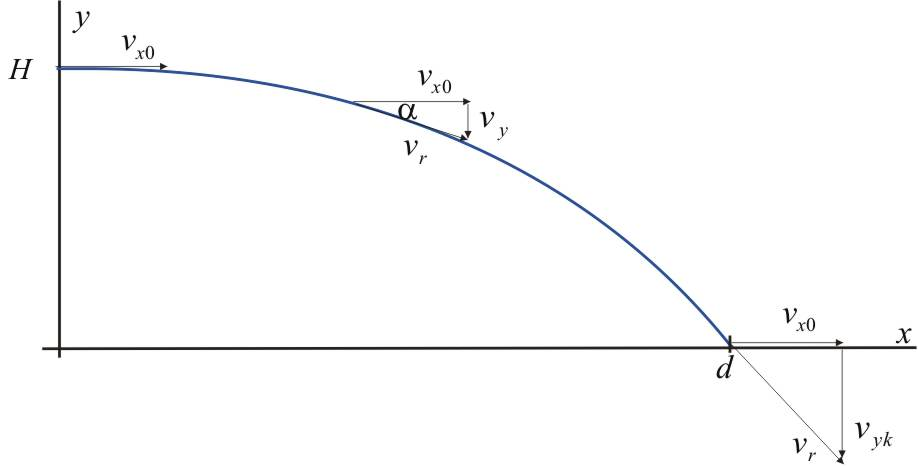
\includegraphics[width=0.5\linewidth]{MotoParabolico.jpg}
    \caption{Moto Parabolico}
    \label{fig:enter-label}
\end{figure}
\noindent
Solitamente il moto parabolico si compone di due moti: lungo l'asse delle \textbf{x} abbiamo un \textbf{moto rettilineo uniforme}, in cui troviamo v costante. Per questo motivo prendiamo la legge oraria della posizione del moto rettilineo uniforme:
\begin{equation}
    x=vt + x_0=v_{0x}t + x_0 = v_0cos(\alpha)t + x_0
\end{equation}
e sostituiamo a v quella che è solamente la sua componente orizzontale. Ricordando:
\begin{figure}[H]
    \centering
    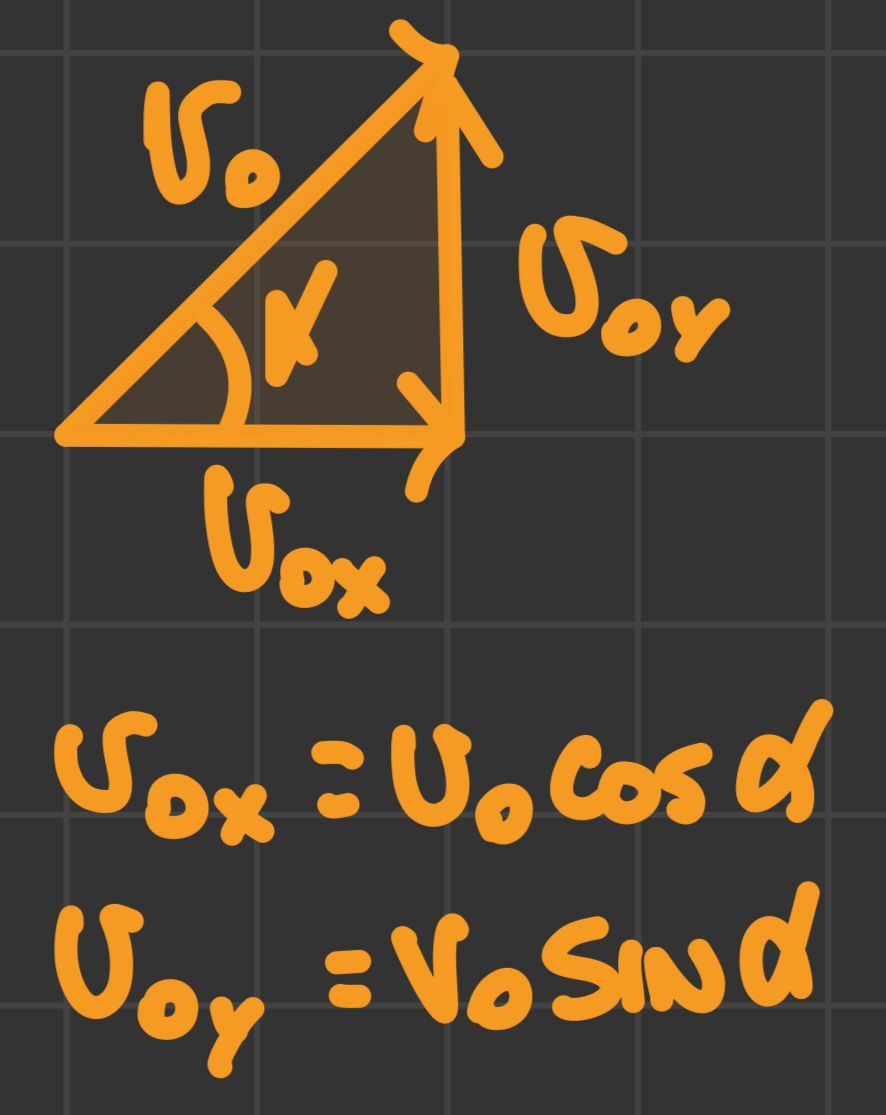
\includegraphics[width=0.25\linewidth]{componenti.jpeg}
    \caption{Componenti}
    \label{fig:enter-label}
\end{figure}
\noindent
Lungo l'asse delle \textbf{y} vi è un \textbf{moto rettilineo uniformemente accelerato}, quindi con a costante. Prendiamo quindi la legge oraria della posizione in un moto rettilineo uniformemente accelerato.
\begin{equation}
    y=y_0+v_{0y}t + \frac{1}{2}at^2=y_0+v_0sin(\alpha)-\frac{1}{2}gt^2
\end{equation}
Consideriamo solamente la componente verticale della velocità e introduciamo g come la gravità=$9.8 \ m/s^2$. La parte dell'accelerazione cambia di segno perchè la forza di gravità spinge verso il basso rispetto all'orientamento che abbiamo preso per l'asse y. Le principali applicazioni del moto parabolico sono nella balistica. Alcune osservazioni: troviamo in questo moto degli elementi nuovi come la \textbf{gittata}, la quale rappresenta il punto in cui cade il corpo. Da notare che quando il corpo cade la \textbf{y vale 0}, il che tornerà utile per gli esercizi. Troviamo poi l'\textbf{altezza massima} la quale rappresenta il \textbf{vertice} della parabola, bisogna quindi fare un ragionamento, in ogni punto della curva si può disegnare la direzione della velocità essendo la \textbf{velocità tangente alla curva (sempre)}. Nel punto in cui si ha l'\textbf{altezza massima}, abbiamo \textbf{solo componente orizzontale}. Ideologicamente quindi si può trovare il tempo a partire dalla componente verticale posta a zero della velocità e sostituirlo poi nelle leggi orarie x y per trovare le incognite. Un'altra richiesta degli esercizi è al suolo quanto vale in modulo la velocità e la sua direzione. Ovviamente intende dire un infinitesimo prima, non è zero. Mentre per quanto riguarda la direzione intende l'angolo formato dalle componenti. Il modulo lo troviamo facendo il \textbf{teorema di pitagora} tra le componenti (ovviamente le componenti sono le componenti calcolate per t=tempo di volo/al suolo), mentre l angolo sfruttando questa legge trigonometrica:
\begin{figure}[H]
    \centering
    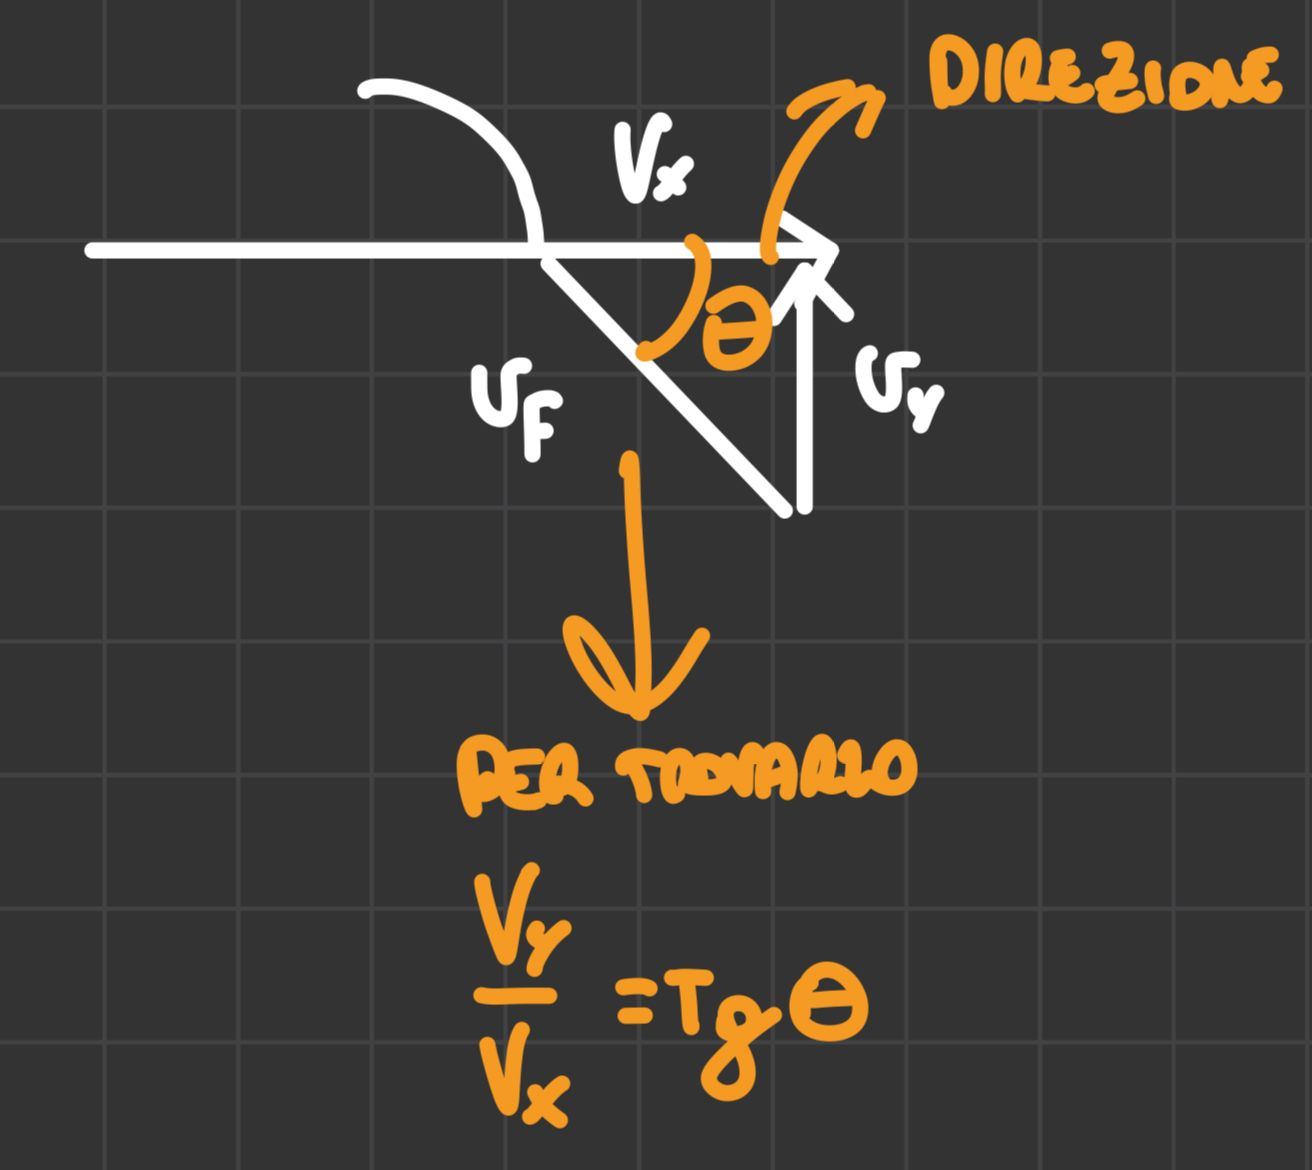
\includegraphics[width=0.5\linewidth]{ModuloEDirezione.jpeg}
    \caption{Modulo e direzione della velocità}
    \label{fig:enter-label}
\end{figure}
\newpage
\section{Lezione 2}
\subsection{Moto Circolare Uniforme}
\begin{figure}[H]
    \centering
    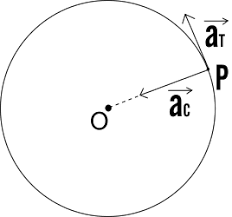
\includegraphics[width=0.25\linewidth]{MotoCircolare.png}
    \caption{Accelerazione Tangenziale e Centripeta}
    \label{fig:enter-label}
\end{figure}
\noindent
Il moto circolare uniforme, come il moto parabolico, è un moto nel piano e segue quindi gli assi x e y. Essendo il moto un moto uniforme, ci troviamo in presenza di una velocità costante in cui però sono presenti dei cambi di direzione, ricordandoci che la velocità è sempre tangenziale alla traiettoria (la curva) ci chiediamo, essendo costante e quindi non cambiando in modulo ma avendo dei cambi di direzione, cosa succede all'accelerazione? Quando parliamo di moto circolare che sia uniforme o uniformemente accelerato, dato che la velocità cambia di direzione, abbiamo un accelerazione, detta \textbf{accelerazione centripeta}. 
\begin{equation}
    a_c=\frac{v^2}{R}
\end{equation}
Essendo questa la formula, notiamo che maggiore sarà la velocità e maggiore sarà l accelerazione centripeta. Adesso ci interessa capire perchè l'\textbf{accelerazione centripeta è radiale.} Ovvero punta sempre verso il centro della traiettoria, entra dal corpo e va nel centro della traiettoria. Abbiamo una velocità costante lungo la traiettoria, considerando che la velocità è sempre tangente alla curva, avremo che l'\textbf{accelerazione tangenziale} sarà = 0. Dato che l'accelerazione tangenziale e l'accelerazione centripeta descrivono l'accelerazione totale, l'accelerazione centripeta potrà essere l'unico componente che può provocare un cambio di direzione senza incidere sulla traiettoria, essendo quest'ultima \textbf{ortogonale ad essa}. Infatti se la velocità cambia nel tempo, avremo che anche cambierà anche l'accelerazione tangenziale, quando la v cambia, cambia anche direzione giustificando la natura radiale dell'accelerazione centripeta. Un'altra osservazione rilevante è che quando il \textbf{raggio di curvatura della traiettoria tende all'infinito}, la traiettoria e sempre meno curva e di conseguenza il moto sarà tendente a un moto \textbf{rettilineo} di fatti l'accelerazione centripeta tenderà a 0. \\ \\
Andiamo poi a introdurre il \textbf{periodo} del moto circolare, che corrisponde al \textbf{tempo impiegato dal punto per compiere un giro completo.} Importante notare come il periodo, esiste solo nel moto circolare uniforme e non nell'uniformemente accelerato dato che la velocità, variando, non ci permette di stabilire un periodo. Il suo \textbf{reciproco} è la frequenza che corrisponde a \textbf{quanti giri faccio al secondo} si misura in Hertz che corrispondono a $s^{-1}$. \\ \\ 
Ci chiediamo ora quanto valga la velocità in un moto rettilineo uniforme:
\begin{equation}
    v=\frac{\Delta x}{\Delta t}=\frac{2 \pi R}{T}
    \end{equation}
C'è ora da precisare, che quando spazi un arco stai spaziando anche un angolo nell'unità di tempo introduciamo per questo la \textbf{velocità angolare}:
\begin{equation}
    \omega=\frac{2 \pi}{T}
\end{equation}
Ricordandoci quanto vale la velocità troviamo che:
\begin{equation}
    v = \omega R
\end{equation}
\begin{figure}[H]
    \centering
    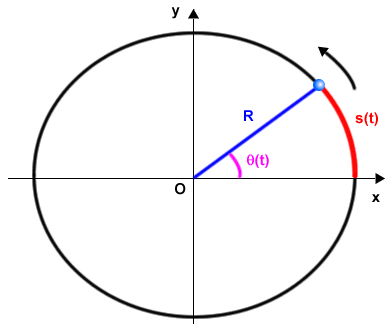
\includegraphics[width=0.5\linewidth]{MotoCircolareUniforme.png}
    \caption{Moto Circolare Uniforme}
    \label{fig:enter-label}
\end{figure}
\noindent
Vogliamo ora cercare di introdurre le leggi orarie o la legge oraria del moto circolare uniforme e vorremmo scriverla nel tempo. Abbiamo detto che questo è un moto nel piano e quindi abbiamo sia y che x. Descrivere entrambi ci risulterebbe complicato a livello matematico, una giustificazione, potrebbe essere data dal fatto che una circonferenza non è una funzione. Capiamo che i moti di x e y dipendono tra loro, allora potremmo scrivere solo una legge tra le due, ma sarebbe comunque complicato. Osserviamo allora l'\textbf{angolo} che forma il punto con l'origine rispetto all'asse orizzontale. Dato l'angolo infatti con le leggi trigonometriche possiamo capire sia x e y, per questo motivo parliamo di \textbf{posizione angolare} ed è la \textbf{legge oraria} del moto circolare uniforme:
\begin{equation}
    \theta(t)=\omega t + \theta_0
\end{equation}
Ovviamente come per il moto rettilineo uniforme, se $\theta_0=0$ allora la posizione angolare equivale allo spazio angolare percorso. In questo moto abbiamo \textbf{$\omega $ costante}.
\newpage
\subsection{Moto Circolare Uniformemente Accelerato}
Essendo un moto accelerato, siamo in presenza di un accelerazione che non appare nel moto circolare uniforme, ovvero l'accelerazione tangenziale. Capita l'analogia con i moti rettilinei andiamo a scrivere le \textbf{leggi orarie} del moto circolare uniformemente accelerato:
\begin{align}
   &  \theta(t)=\theta_0+\omega_0t+\frac{1}{2}\alpha t^2 \\
   &  \omega(t)= \alpha t + \omega_0
\end{align}
Introducendo alpha come l'\textbf{accelerazione angolare}. Notiamo come la velocità angolare sia la derivata della \textbf{posizione angolare}. Andiamo ora a fare dei ragionamenti sulle accelerazioni per trovare delle formule utili:
\begin{equation}
    a_c=\frac{v^2}{R}= \omega^2 R
\end{equation}
Abbiamo sostituito la formula della velocità. Ricordandoci ora che la velocità è tangenziale e l'accelerazione pure:
\begin{equation}
    \frac{dv}{dt}=\frac{d(\omega R)}{dt} \ \ \  -> \ \ \ \frac{dv}{dt}=R \frac{d\omega}{dt}=R \alpha
\end{equation}
Troviamo l'accelerazione tangenziale:
\begin{equation}
    a_T=\frac{dv}{dt}=R \alpha
\end{equation}
Ricordandoci della situazione della figura 4, troviamo l'accelerazione totale come la somma pitagorica tra le accelerazioni precedentemente introdotte:
\begin{equation}
    a=\sqrt{a_T^2 + a_c^2}
\end{equation}
\begin{figure}[H]
    \centering
    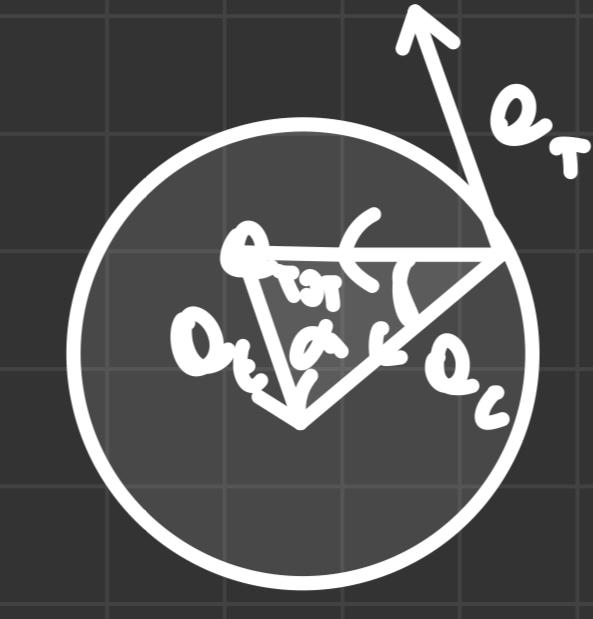
\includegraphics[width=0.25\linewidth]{AngoloAccelerazione.jpeg}
    \caption{Angoli tra le accelerazioni}
    \label{fig:enter-label}
\end{figure}
\noindent
Potrebbero chiedere l'angolo che forma l'accelerazione totale con la normale e come per la velocità nel moto parabolico. Se dovessero chiedere l'angolo con la tangenziale, basta fare 90-questo sotto oppure invertire i divisori.
\begin{equation}
    tg(\alpha)=(\frac{a_T}{a_c})
\end{equation}
\subsection{Moto Armonico}
\begin{minipage}[t]{0.4\textwidth}
  \raisebox{-\height}{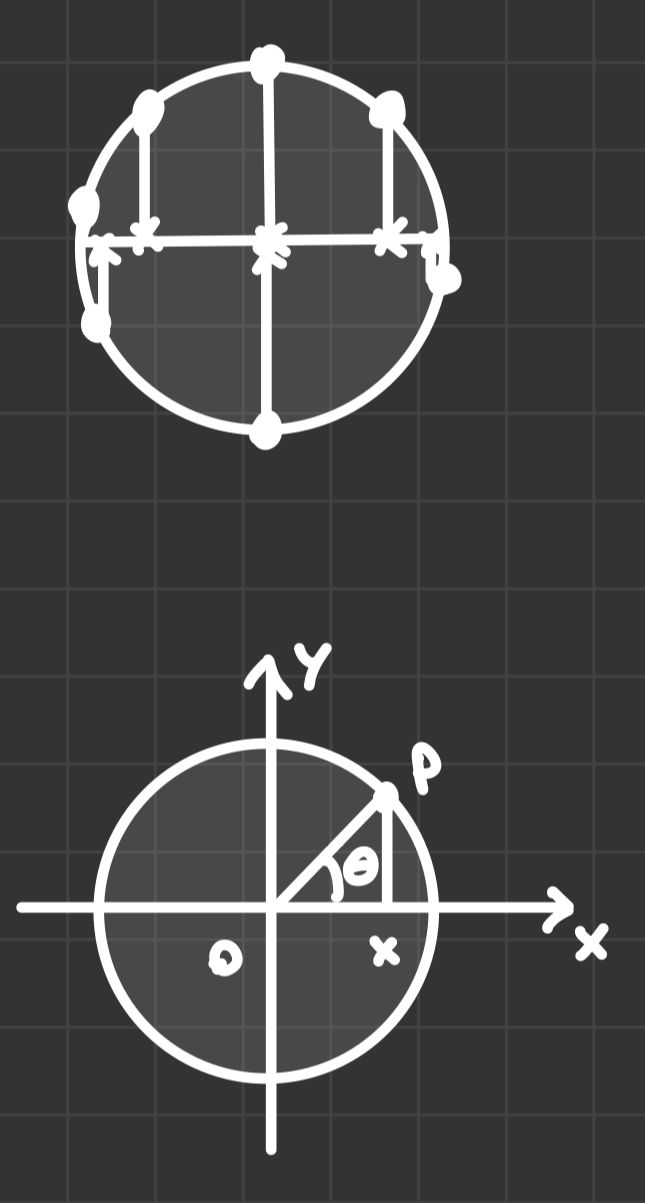
\includegraphics[width=\linewidth]{MotoArmonico.jpeg}}
\end{minipage}%
\hfill
\begin{minipage}[t]{0.55\textwidth}
  \raggedright
Il moto Armonico, non è strettamente riconducibile ad un moto circolare, ma per introdurlo, facciamo dei ragionamenti relativi ad un moto circolare. Prendiamo dei punti sulla circonferenza e li proiettiamo su di un diametro, se il punto compie un giro, significa che ha attraversato il diametro che rappresenta un moto rettilineo. Questo moto detto \textbf{armonico} ha una particolare legge della posizione. Il punto P forma un angolo rispetto all'asse orizzontale, la sua proiezione sul diametro ci permette di trovare la x. La x è quindi:
\begin{equation}
    x=Rcos\theta
\end{equation}
Ovviamente $\theta$ può variare nel tempo, per questo motivo ricordandoci della \textbf{legge oraria del moto circolare uniforme} otteniamo:
\begin{equation}
    x=Rcos(\omega t + \theta_0)=Acos(\omega t + \theta_0)
\end{equation}
Dove R in realtà corrisponde a A che è l'\textbf{ampiezza del moto armonico}. $\theta_0$ è la fase iniziale. $\omega$ invece è la \textbf{pulsazione}. In questo moto, l'accelerazione non è costante, per questo motivo deriviamo la legge oraria della posizione:
\begin{equation}
    v=-\omega A sen(\omega t+\theta_0)
\end{equation}
Essendo 1 il valore massimo del seno abbiamo che la velocità massima in modulo è uguale a:
\begin{equation}
    v_{max}=\omega A
\end{equation}

\end{minipage}
Ovviamente posso scambiare i seni e i coseni se giovano vantaggi in funzione dei calcoli. Seno e coseno sono in \textbf{quadratura di fase}, ovvero sono sfasati di 90 gradi quindi quando la velocità è massima, la posizione è uguale a 0. Capiamo dalla formula della velocità che che quest'ultima non è costante deriviamo e troviamo la formula dell'accelerazione:
\begin{equation}
    a=-\omega^2Acos(\omega t + \theta_0)
\end{equation}
Anche qui il valore massimo del coseno è uno e troviamo quindi:
\begin{equation}
    a_{max}=\omega^2A
\end{equation} 
Posizione e accelerazione sono quindi massime con segno discorde.
\section{Lezione 3}
\subsection{Seconda legge di Newton}
In questa lezione andiamo a iniziare il primo argomento che faremo della \textbf{dinamica}, la quale si occupa di studiare le cause del moto. Il legame tra la dinamica e la cinematica è la \textbf{seconda legge di Newton}. La quale ci dice che: \textbf{l'accelerazione ci lega alle cause, ogni volta che vi è un'accelerazione vi è una forza.}
\begin{equation}
    \sum_i\vec{F}=m\vec{a}
\end{equation}
Ovviamente più è grande la massa e più piccola sarà l accelerazione rispetto ad essa e più fatica faremo a cambiarne la velocità, per questo parliamo di: \textbf{Principio inerziale}. Notare come la F sia una sommatoria questo perchè equivale alla risultante delle forze. 
\subsection{Esercizi}
Questa parte la spiegheremo maggiormente con gli esercizi (vedi ipad). La prima cosa che si fa con gli esercizi di dinamica è quella di \textbf{disegnare tutte le forze}. Bisogna capire il collegamento che vi è tra cinematica e dinamica. Quando parliamo di forze abbiamo perforza un'accelerazione il che implica un moto uniformemente accelerato. Per questo motivo, possiamo utilizzare le formule del moto per determinare \textbf{velocità}, \textbf{tempo}, \textbf{spostamento}. 
\subsubsection{Forza d'attrito}
Parliamo poi di \textbf{forza d'attrito} la quale è sempre parallela alla traiettoria ma si oppone al moto possibile.
\begin{equation}
    \vec{F}_{attr}=\mu N
\end{equation}
Questa è la formula della forza d'attrito in cui però dobbiamo avere delle accortezze. Quando il corpo è fermo abbiamo che (F è una generica forza che spinge il corpo):
\begin{equation}
    \vec{F}-\vec{F}_{attr}=0 \ \ \ \ \xrightarrow[]{} \ \ \ \ \vec{F}=\vec{F}_{attr}
\end{equation}
La formula che abbiamo introdotto prima, è la formula relativa a \textbf{quando il corpo si muove e perciò significa che la forza d'attrito non riesce più a opporsi perchè ha raggiunto il suo massimo.} Il problema nasce dal fatto che: \textbf{se il corpo è fermo, non sappiamo se la forza d'attrito ha raggiunto il suo massimo.} Per cui non possiamo calcolarla. La possiamo calcolare nel caso in cui il testo ci da delle motivazioni o dice che il corpo sta per muoversi (al distacco). Quindi nel caso in cui possiamo usarla N è la \textbf{reazione che il piano ha ortogonalmente a se stesso.} Solitamente su un piano orizzontale è la \textbf{forza peso mg} se siamo su un piano inclinato non è totalmente la forza peso, ci torniamo dopo. 
\subsubsection{Tensione di filo}
Modifichiamo gli esercizi, prendendo in considerazione più punti materiali, due in particolare, collegati da un filo inestensibile di massa trascurabile, in un "sistema" l'accelerazione dei corpi è sempre la stessa, per questo motivo per calcolare l'accelerazione di un corpo conviene considerare tutto il sistema. Infatti se volessimo calcolare la reagente di un solo corpo o la sua accelerazione dovremmo considerare anche la \textbf{tensione del filo}. Infatti nel caso di tutto il sistema non la consideriamo, dato che quando abbiamo un filo abbiamo sempre una \textbf{coppia di tensioni opposte}. Per ogni tratto di filo vi è una coppia di tensioni.
\subsubsection{Piano Inclinato}
\begin{minipage}[t]{0.4\textwidth}
  \raisebox{-\height}{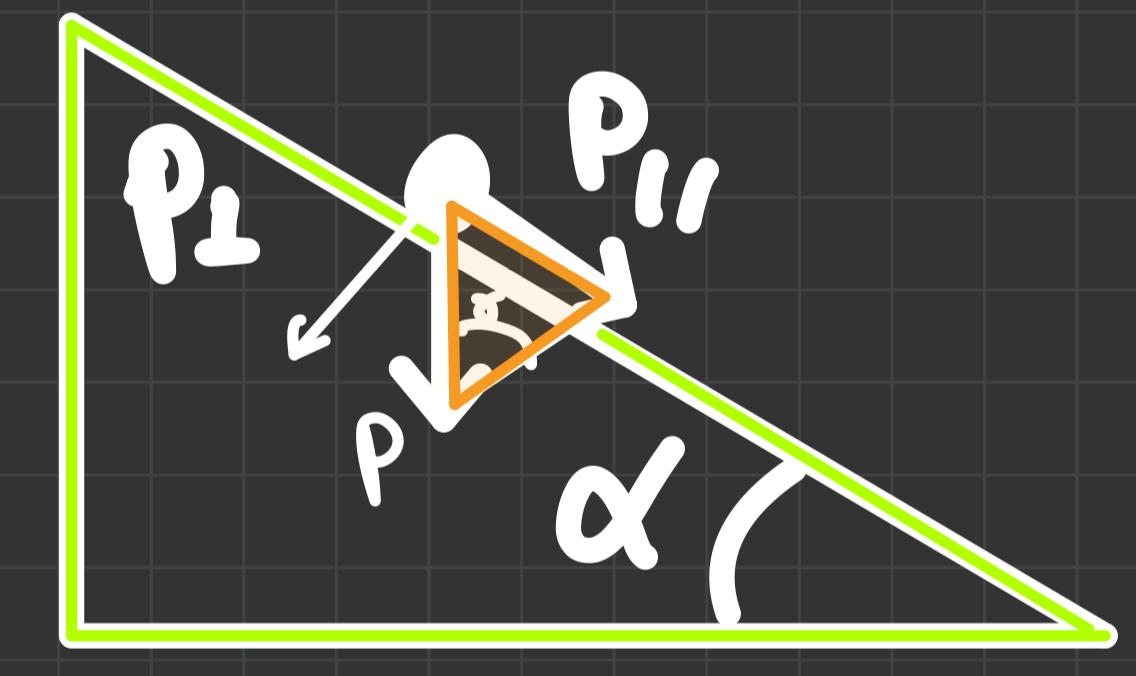
\includegraphics[width=\linewidth]{PianoInclinato.jpg}}
\end{minipage}%
\hfill
\begin{minipage}[t]{0.55\textwidth}
  \raggedright
Consideriamo ora un ulteriore variazione dell'esercizio, questa volta teniamo conto di un piano inclinato. Le forze essendo dei \textbf{vettori} hanno ovviamente delle componenti, in particolare la \textbf{forza peso}, va proiettata lungo la direzione del movimento, dando luogo a una $P_\parallel$ e una $P_\perp$. Notiamo dall'immagine che l'angolo formato dalle componenti della forza peso è \textbf{lo stesso} formato dal piano inclinato, parliamo quindi di \textbf{omotetia}, infatti i due triangoli (arancione e verde) hanno gli stessi angoli con i lati proporzionali. Per cui avremo considerando $P_\parallel$ come cateto e la forza peso P come ipotenusa:
\begin{equation}
    P_\parallel=Psin(\alpha) \ \ \ \ , \ \ \ \ P_\perp=Pcos(\alpha)
\end{equation}

\end{minipage}
Importante notare, come la componente che spingerà il corpo verso il piano inclinato sarà la componente \textbf{parallela}, mentre la componente che si opporrà al moto sarà la componente \textbf{perpendicolare} che sarà quindi la reazione vincolare. Essendo la forza peso $P=mg$ non avremo bisogno della massa per calcolare l'accelerazione:
\begin{equation}
    a=\frac{P_\parallel}{m}=\frac{mgsin(\alpha)}{m}=gsin(\alpha)
\end{equation}
\subsubsection{Inclinazione della forza}
Consideriamo ora una forza che viene data con un certo angolo. Essendo quest'ultima inclinata avrà due componenti, una sull'asse x e una sull'asse y. Quella sull'asse y ovviamente influirà sulla \textbf{forza peso} e si andrà a sottrarre a quest'ultima nel caso in cui vogliamo calcolare la \textbf{reazione vincolare}. La forza quindi che favorirà il moto ed anche la forza che andiamo a considerare è la \textbf{componente orizzontale}.
\subsubsection{Molla}
La molla è uno strumento che si allunga e si accorcia. Essa ha una \textbf{costante di rigidezza K} espressa in N/m che ci dice con quanta facilità si allunga la molla. La molla esprime una \textbf{forza di richiamo} su di un corpo attaccata ad essa. Enunciamo quindi la \textbf{legge di Hooke} la quale descrive la \textbf{forza elastica}:
\begin{equation}
    F=-k\Delta x
\end{equation}
Il meno è dato dal fatto che essendo una forza di richiamo va nel lato opposto, infatti se comprimo fa il contrario. Una cosa a cui bisogna fare attenzione, è il caso in cui la \textbf{molla si trova all'interno di un filo che ha tensione.} Di base la molla non ha massa, e quindi non la prendo in considerazione, essendo la forza elastica interna al sistema, non entra in gioco. Una domanda potrebbe essere \textbf{Di quanto si allunga la molla?} In questo caso, la forza elastica è data dalla tensione del filo quindi:
\begin{equation}
    \Delta x=\frac{T}{k}
\end{equation}
Infatti dovrei per prima cosa calcolare la tensione, dato che la molla si allunga grazie alla tensione. Ultime accortezze: quando abbiamo un moto uniforme non abbiamo accelerazione e di conseguenza neanche forza, se dobbiamo calcolare una tensione di filo, conviene prendere in considerazione il corpo che ha in ballo meno pezzi di filo possibile. Nel caso dell esercizio n.2 del 6 febbraio 2023 quando chiede se si accorcia la distanza lo giustifichiamo in questo modo: essendo la forza d attrito diversa, è chiaro che uno dei due punti farà più strada, voglio quindi calcolare la legge oraria dei due, per farlo scrivo la legge oraria del moto uniformemente accelerato, trovando come incognite il tempo l accelerazione e lo spazio. Trovo l accelerazione con la forza, sappiamo che la velocità quando si fermano sarà uguale a 0 per cui trovo il tempo e successivamente trovo lo spazio percorso.
\section{Lezione 4}
\subsection{Introduzione}
Andiamo a introdurre quelli che sono i concetti di \textbf{energia e lavoro}. L'esigenza nasce dal fatto che ci sono esercizi in cui non si può applicare direttamente la dinamica o comunque il \textbf{metodo energetico} ci facilita la vita. Con il metodo energetico non possiamo però calcolare il tempo, che calcoleremo con le leggi orarie e le reazioni vincolari, che calcoleremo con le equazioni della dinamica. Il metodo energetico non esclude i risultati che abbiamo già visto della dinamica.
\newpage
\subsection{Lavoro di una forza}
Andiamo a parlare generalmente di lavoro e cos'è prima di andarlo a definire.
\begin{figure}[H]
    \centering
    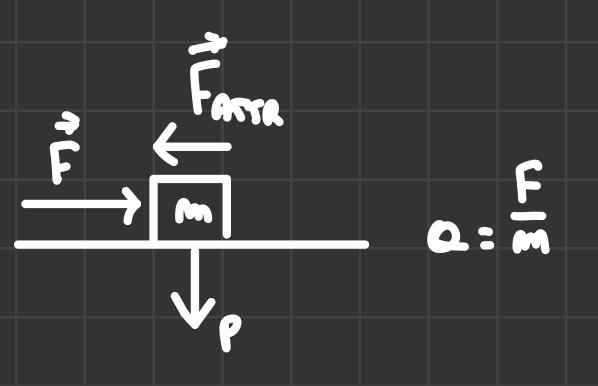
\includegraphics[width=0.5\linewidth]{Lavoro.jpeg}
    \caption{}
    \label{fig:enter-label}
\end{figure}
Sappiamo che applicata una forza, avremo un moto uniformemente accelerato per un certo istante di tempo, il quale ci farà compiere uno spostamento. Abbiamo quindi che il lavoro sarà:
\begin{equation}
    W=F \vec{s}
\end{equation}
Prendiamo ora in considerazione l'attrito. Anche quando agisce l'attrito abbiamo lavoro:
\begin{equation}
    W=-F_{attr} \vec{s}
\end{equation}
Consideriamo ora anche la forza peso e ci chiediamo se questa produca lavoro. Capiamo che \textbf{produce lavoro solamente una forza che ha una componente parallela allo spostamento}, in questo caso la forza non partecipa allo spostamento.
\begin{equation}
    W_p=0
\end{equation}
Quindi la formula che generalizza le tre precedenti è:
\begin{equation}
    W=F\vec{s}cos(\alpha)
\end{equation}
Dove $\alpha$ è l'angolo tra la direzione dello spostamento e la direzione della forza. Prima abbiamo detto che nel metodo energetico non rientrano le reazioni vincolari, perchè? Perchè le reazioni vincolare sono sempre ortogonali allo spostamento.
\subsection{Energia}
Iniziamo a parlare di \textbf{sistema corpo}, nella dinamica il sistema corpo veniva "ufficializzato" dalla massa in $F=ma$, dal punto di vista energetico, ci riferiamo al sistema, il quale può avere più contributi in un dato istante di tempo:
\begin{itemize}
    \item \textbf{Energia Cinetica $E_k$}: è quell'energia che un corpo ha perchè è in moto ($v\neq 0$)
    \begin{equation}
        E_k=\frac{1}{2}mv^2
    \end{equation}
    Notare come quando parliamo di lavoro e energia i contributi sono scalari e quindi danno luogo a una sola equazione, le forze invece, hanno più direzioni.
    \item \textbf{Energia Potenziale Gravitazionale $E_{pg}$}: è quell'energia che un corpo di massa m si trova ad avere se si trova in un campo gravitazionale
    \begin{equation}
        E_{pg}=mgh
    \end{equation}
    Dove h è la quota che scegliamo arbitrariamente a seconda della nostra convenienza, infatti alle volte questo può esserci utile dato che quando $h=0$ anche $E_{pg}=0$. Facciamo un esempio, lancio una palla dal quarto piano e mi chiedo se questa ha energia potenziale, se prendo come riferimento il suolo ovviamente h sarà l'altezza del palazzo al quarto piano, quindi ha energia potenziale che al suolo si tramuta in energia cinetica. Quest'energia cinetica, la avevo in potenza al quarto piano. Se invece prendo $h=0$ al quarto piano allora l'energia potenziale sarà zero, però questo non esclude che non possa avere energia, ovviamente al quarto piano la velocità era pari a 0.
    \item \textbf{Energia Potenziale Elastica $E_{pe}$}: questa la capiamo facendo un esempio, comprimo una molla con una certa forza, se la lascio arriva in posizione di riposo con una certa velocità, il che vuol dire che avevo immagazinato energia. Ovviamente lo stesso discorso vale quando la allungo, questa energia la troviamo solamente in presenza di una molla.
    \begin{equation}
        E_{pe}=\frac{1}{2}k\Delta x^2
    \end{equation}
\end{itemize}
\subsection{Equazione di conservazione dell'energia meccanica}
Introduciamo l'\textbf{energia meccanica} come:
\begin{equation}
    E_m=E_k + E_{pg}+E_{pe}
\end{equation}
Ovviamente non è detto che i contributi delle energie ci siano tutti. Troviamo invece la \textbf{variazione di energia meccanica} come (essendo questa una variazione, compresa tra due istanti di tempo, è importante considerarla in istanti in cui ho dati dal testo o in cui cerco incognite):
\begin{equation}
    \Delta E_m=\sum_i W_{nc}
\end{equation}
\newpage
\subsubsection{Forze conservative e non}
\begin{minipage}[t]{0.4\textwidth}
  \raisebox{-\height}{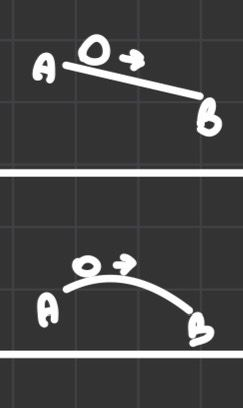
\includegraphics[width=\linewidth]{ForzeNonConservative.jpeg}}
\end{minipage}%
\hfill
\begin{minipage}[t]{0.55\textwidth}
  \raggedright
Definiamo cosa sono le forze \textbf{conservative e non conservative}, per avere più chiaro il quadro sull'energia. Prendiamo un generico punto materiale su un piano orizzontale a cui viene applicata una forza, avremo quindi un attrito che si opporrà al moto. Il suo lavoro sarà quindi uguale a:
\begin{equation}
    W_{attr}=-F_{attr} * \overline{AB}
\end{equation}
Adesso prendiamo un 'altro tratto, questa volta curvilineo. Abbiamo che il lavoro della forza d'attrito sarà come prima ad eccezione dello spostamento, infatti essendo il tratto curvo, stiamo percorrendo più strada rispetto a quella che percorrevamo prima. Questo succede anche perchè l'attrito è sempre tangente alla traiettoria. Di conseguenza se il \textbf{lavoro dipende dalla traiettoria, la forza non è conservativa.} 
\end{minipage}
Consideriamo ora un piano inclinato per vedere come si comportano le \textbf{forze conservative}.
\begin{figure}[H]
    \centering
    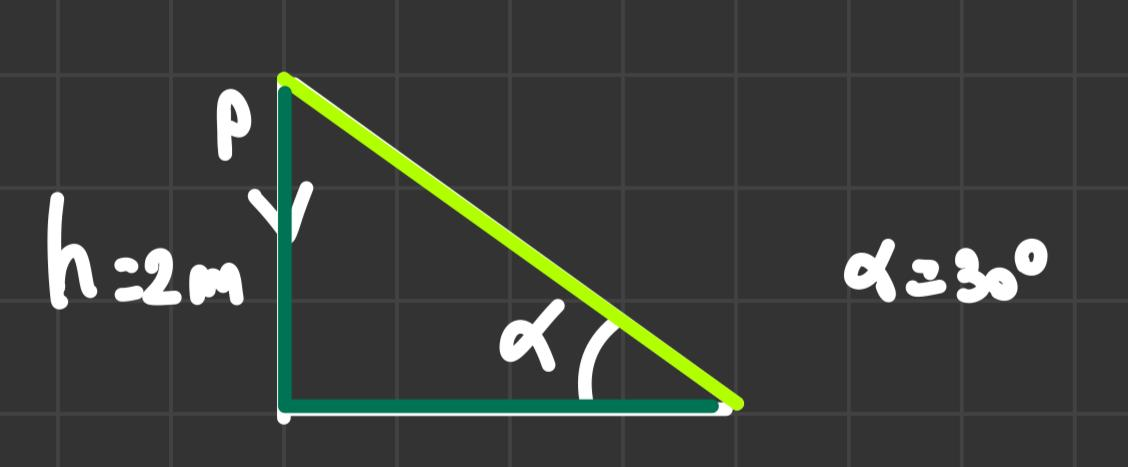
\includegraphics[width=0.5\linewidth]{ForzeCOnservative.jpeg}
    \label{fig:enter-label}
\end{figure}
\noindent
Per calcolare il lavoro, possiamo percorrere due percorsi, iniziando da quello verde scuro, abbiamo che la forza peso spinge verso il basso, lo spostamento è verso il basso:
\begin{equation}
    W=P * h=mgh
\end{equation}
successivamente gira a destra e la forza peso diventa ortogonale alla traiettoria e quindi $W=0$. Se consideriamo invece il tratto in verde chiaro, abbiamo che:
\begin{equation}
    W=P_\parallel*scos(0) = mgsin(\alpha)*s=mgh
\end{equation}
Il cos è di 0 dato che non si forma nessun angolo tra la traiettoria e la forza peso parallela. Abbiamo che essendo $s*sin(\alpha)$ proprio il tratto h, il lavoro non dipende dalla traiettoria. Quindi una \textbf{forza conservativa ammette un lavoro che non dipende dalla traiettoria}. Le forze non conservative sono: le\textbf{forze esterne al sistema} e la \textbf{forza d'attrito}.
\subsubsection{Esempio}
Vediamo un esempio con un piano inclinato e alla base vi è una molla. Voglio capire di quanto si comprime la molla. Per farlo ho bisogno dell energia. \textbf{Come si usa l'equazione di conservazione dell'energia meccanica}: Solitamente, quello che facciamo è, calcolare il lavoro delle forze non conservative, ed eguagliarlo alla variazione dell'energia meccanica. L'energia meccanica l'abbiamo introdotta come la somma delle tre di fatti, prendo l'energia meccanica iniziale (che nell'esempio è l'energia potenziale e basta) prendo l'energia meccanica finale (che nell'esempio è energia potenziale gravitazionale (la quale però è 0) e energia potenziale elastica), sottraggo la finale all'iniziale, la impongo uguale al lavoro delle forze non conservative e da quest'equazione trovo l'incognita, che in questo caso è di quanto si comprime la molla. Su quest'esercizio altre note importanti sono: abbiamo trovato lo spostamento considerando il piano inclinato come un triangolo rettangolo e quindi trovandone l'ipotenusa.
\subsection{Problema del giro della morte (Esame 19 giugno)}
\begin{figure}[H]
    \centering
    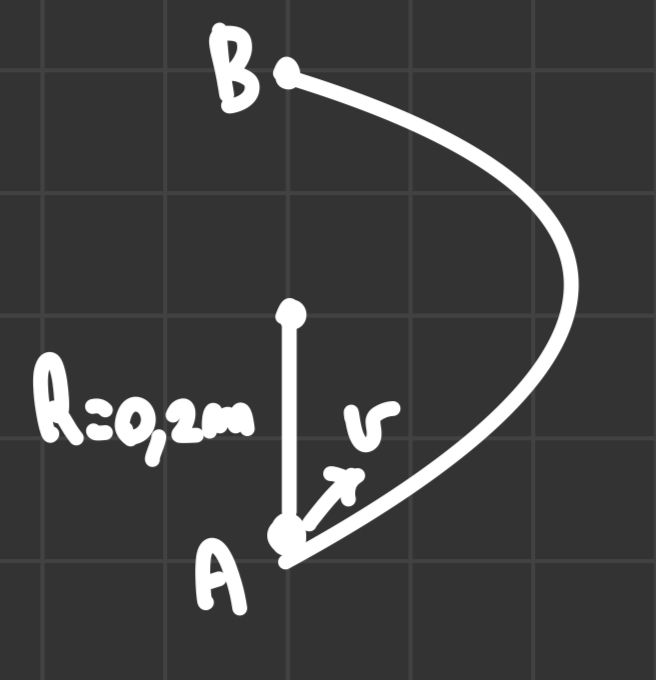
\includegraphics[width=0.25\linewidth]{GiroDellaMorte.jpeg}
    \caption{Problema del giro della morte}
    \label{fig:enter-label}
\end{figure}
\noindent
Il problema richiede, la velocità v che il punto deve avere nel punto a, in modo tale che non si stacchi fino a b. Quello che vogliamo quindi è che si arrivi in b con $v>0$. Quindi, ho un energia cinetica iniziale, ne ho una potenziale finale e spero di avere anche un'energia cinetica finale. Quest'esercizio, è una combo tra dinamica, cinematica e energia. Quindi, per quanto riguarda la dinamica, in B avremo, la forza peso e la reazione vincolare della guida. Per la cinematica invece, osserviamo che il punto per mantenere il moto lungo la guida fa un moto circolare, di conseguenza, anche in b avremo moto circolare e saremo quindi in presenza di accelerazione centripeta. In realtà siamo in presenza di accelerazione centripeta dato che P e R puntano verso il centro. Quindi:
\begin{equation}
    P+R=ma_c
\end{equation}
Ricordando che:
\begin{align}
    & a_c=\frac{v^2}{r} \\
    & P+R=m *\frac{v^2}{r}
\end{align}
Il testo ci chiede in realtà quando deve valere $v_a$ in modo tale che il punto possa al minimo fare il giro della morte? Dobbiamo quindi arrivare ad avere una situazione in cui R=0 ovvero stiamo imponendo una condizione limite in cui per R=0 il corpo sta per staccarsi. Avremo quindi:
\begin{equation}
    P=m*\frac{v^2}{r} \xrightarrow[]{}mg=m*\frac{v^2}{r}\xrightarrow{}g=\frac{v^2}{r}\xrightarrow{}v=\sqrt{gr}=1.4 \  m/s^2
\end{equation}
Troviamo quindi la velocità minima che il punto deve avere in b. Devo quindi trovare $v_a$, ricordandomi che agiscono solo forze conservative, abbiamo che:
\begin{equation}
    \Delta E_m=W_{nc} \xrightarrow[]{} \Delta E_m=0 \xrightarrow[]{} E_{m, iniziale}=E_{m, finale}
\end{equation}
Vado quindi a impostare l'equazione:
\begin{equation}
    E_k=E_k+E_{pg} \ \ \ \ \xrightarrow[]{} \ \ \ \ \frac{1}{2}mv_a^2=\frac{1}{2}mv_b^2+mgh
\end{equation}
La v è proprio la velocità in a che stavo cercando.
\subsection{Urti}
Introduciamo \textbf{l'equazione di conservazione della quantità di moto}:
\begin{equation}
    \vec{J}=\vec{F}*\Delta t \ \  [N/s] \ \ [Kg *m/s]
\end{equation}
Dove J è l'\textbf{impulso di una forza} e $\Delta t$ è l'intervallo di tempo da quando ho applicato la forza. Questo concetto è strettamente legato alla \textbf{quantità di moto} dato che fornisce una variazione di quest'ultima:
\begin{equation}
    \vec{q}=m*\vec{v}
\end{equation}
Essendo questa un'equazione vettoriale, è possibile scalarla sugli assi. Nell'impulso, prendiamo in gioco, le forze \textbf{esterne} al sistema, come ad esempio la forza peso e la forza elastica, ovvero tutto ciò che è esterno al sistema corpo. Esistono anche forze \textbf{interne} che sono quelle che si scambiano due corpi, ad esempio la tensione di filo. Quando ho due corpi che urtano tra di loro entrano in gioco le \textbf{forze di contatto}. Nell'urto infatti, agiscono solamente forze interne, generalmente le forze esterne non le considero, a meno che non abbiano una componente lungo il movimento. L'urto generalmente viene approssimato, orizzontalmente, e abbiamo nel caso dell urto che:
\begin{equation}
    \vec{q}_{in}=\vec{q}_{fin}
\end{equation}
Ovvero la \textbf{quantità di moto si conserva}. In un urto abbiamo che le due velocità si scontrano e quindi una delle due deve esser considerata negativa. Distinguiamo tre tipologie di urti:
\begin{itemize}
    \item \textbf{Urto Anelastico Perfetto}: Avviene quando i corpi si sono urtati e non proseguono in maniera distinta la traiettoria, ma proseguono fusi (come un unico corpo) e quindi:
    \begin{equation}
        m_1v_1+m_2v_2=M_{tot}*v_F
    \end{equation}
    questo tipo di urto è comodo dato che tolgo una velocità finale di uno dei due corpi.
    \item \textbf{Urto Anelastico Imperfetto}: I due corpi non rimangono uniti e solitamente quando capita, devo proiettare lungo gli assi
    \begin{equation}
        m_1v_1+m_2v_2=m_1v_1+m_2v_2
    \end{equation}
    Una domanda tipo è: Quant'è l'energia dissipata dall'urto ed è uguale a 
    \begin{equation}
        E_{k,iniziale}-E_{k,finale}
    \end{equation}    \item \textbf{Urto Elastico}: nell'urto elastico, si mantiene costante l'energia cinetica e si conserva la quantità di moto. Solitamente si considera solo l'energia cinetica nell'urto che è utile per trovare le velocità. Il problema dell'energia cinetica è che ha all'interno le velocità che però sono al quadrato. Se le metti a sistema con le q il sistema esce non lineare. A questo vi è una scorciatoia che è questa formula che va imparata a memoria:
    \begin{equation}
        v_1'= \frac{(m_1-m_2)}{(m1+m2)}v_1+\frac{2m_2}{(m_1+m_2)}v_2
    \end{equation}
    \begin{equation}
        v_2'= \frac{(m_2-m_1)}{(m1+m2)}v_2+\frac{2m_1}{(m_1+m_2)}v_1
    \end{equation}
    Le v' sono le velocità finali fuori dall'urto, $v_1$ e $v_2$ sono le velocità iniziali.
\end{itemize}
\section{Lezione 5 (Fine prima tipologia)}
La lezione 5 è stata una lezione in cui abbiamo fatto solamente esercizi. Quindi vediamo solamente alcune cose da fare quando si fanno gli esercizi. Molto importante \textbf{bisogna avere in testa come avviene il fenomeno}. Solitamente il moto armonico, non viene utilizzato, è rarissimo, se non impossibile che venga chiesta un incognita come tempo o spostamento nel moto armonico. Infine, bisogna sempre \textbf{fare il disegno} e farlo bene, in modo tale da avere chiaro il quadro e poter capire e scoprire cose sul testo.
\section{Lezione 6}
\subsection{Introduzione}
Iniziamo oggi a parlare di \textbf{corpo rigido}. Il corpo rigido, è un modello per approssimare un corpo nella realtà, viene detto rigido perchè è indeformabile. Ovviamente è pur sempre un approssimazione, anche se si avvicina di più rispetto alla realtà. Aggiungiamo quindi 3 cose che sono: il corpo rigido riprende la \textbf{geometria dei corpi} di conseguenza il corpo rigido, non sarà un solo punto materiale, ma conterrà \textbf{infiniti punti}. Dato che contiene più punti vi sarà quindi una complessità maggiore nel trattarlo, vogliamo comunque estendere i ragionamenti fatti finora. Il punto materiale, effettuava delle traslazioni lungo il rettilineo, il corpo rigido, ovviamente \textbf{traslerà} a differenza del fatto che ogni suo punto cambierà il suo orientamento attorno a una terna di riferimento ovvero \textbf{ruoterà}. Per capire un pò meglio cosa succede prendiamo il corpo rigido più semplice, \textbf{l'asta} che è un corpo rigido \textbf{monodimensionale}, incernierata al tavolo, ciò significa che ha una \textbf{cerniera}.
\begin{figure}[H]
    \centering
    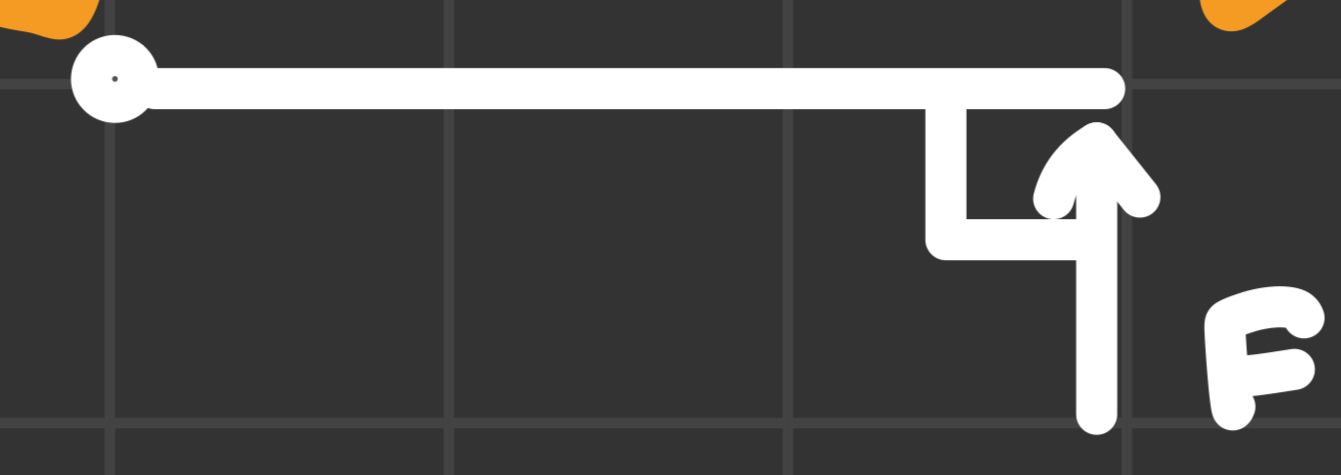
\includegraphics[width=0.5\linewidth]{AstaSemplice.jpeg}
    \label{fig:enter-label}
\end{figure}
\noindent
Questo potrebbe essere potenzialmente, il modello di una porta girevole, infatti quest'asta gira per una causa, la forza di per se procura un'accelerazione ma in traslatoria quindi la causa della rotazione è un altra.
\subsection{Momento di una forza}
\begin{equation}
    M=F*b \ \ \ [Nm]
\end{equation}
Dove b (prima definizione) è la distanza ortogonale tra la cerniera e la direzione della forza. Nota: il momento può esser calcolato rispetto a qualsiasi punto, ovviamente lo calcoliamo rispetto a un punto che può ruotare sennò sarebbe 0. Va chiarita questa definizione di braccio, infatti solitamente forza e braccio, non sono ortogonali come il disegno, la situazione tipo è più la seguente:
\begin{figure}[H]
    \centering
    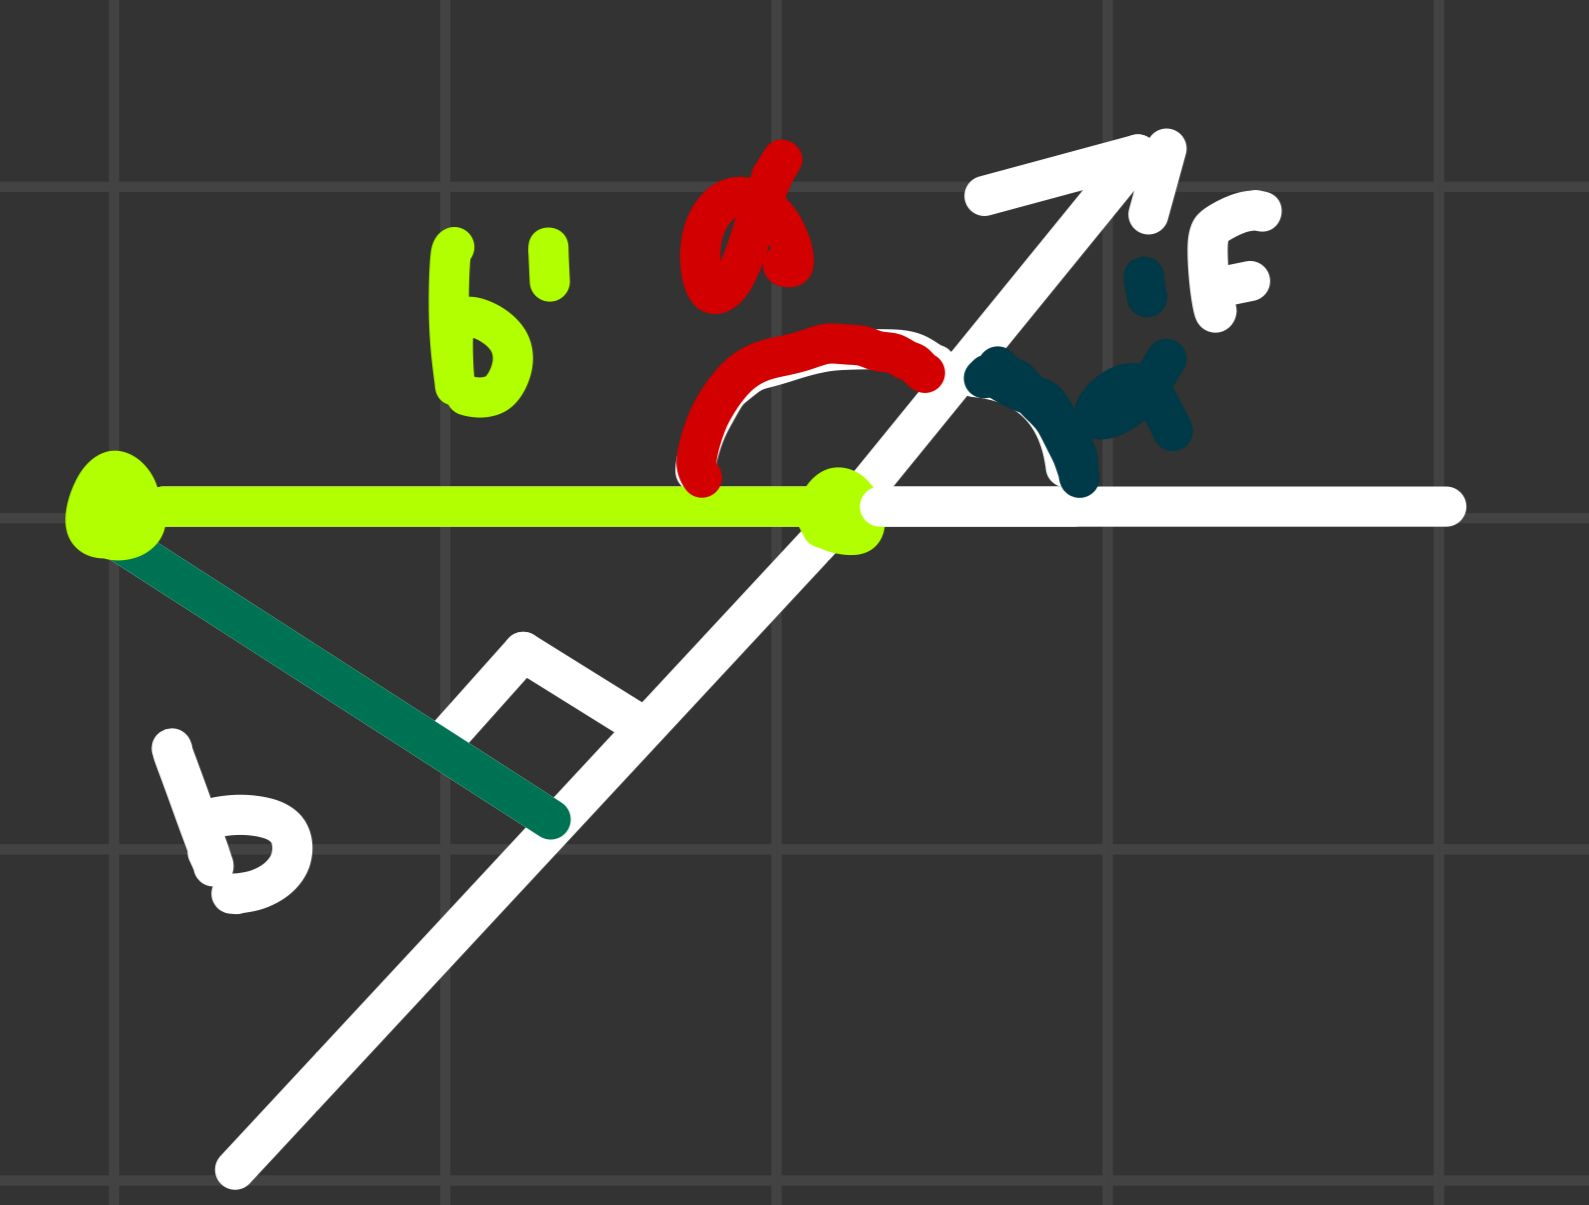
\includegraphics[width=0.3\linewidth]{DefinizioneDiBraccio.jpeg}
    \label{fig:enter-label}
\end{figure}
\noindent
\definecolor{verdeScuro}{HTML}{006400} % verde scuro classico (DarkGreen)
Vi è un angolo diverso tra la direzione dell'asta e la forza, in \textcolor{verdeScuro}{il braccio con l'attuale definizione}, in \textcolor{green}{il braccio con la definizione da seguire per gli *esercizi del borghi}. La definizione di braccio: \textbf{Il braccio è la distanza tra il punto di applicazione della forza e la cerniera}. Troviamo quindi che se la forza non è ortogonale, il \textbf{momento di una forza} sarà dato da:
\begin{equation}
    M=F*b*sin(\alpha)
\end{equation}
Con questo $\alpha$ indico proprio l'angolo formato tra la forza e il braccio, si può utilizzare volendo anche l'angolo complementare, disegnato in figura. Ci sono ovviamente dei casi in cui il momento è nulla: se la forza passa per la cerniera il braccio sarà nullo e il momento anche, il seno può dare 0 o magari do una forza che è parallela all'asta il corpo non si mette a ruotare e il braccio ortogonale è nullo. Il punto da cui vengono calcolati momento e braccio viene detto \textbf{polo}.
\newpage
\subsection{Momento d'inerzia}
Vogliamo tornare a analizzare la causa del movimento di rotazione, sappiamo dalla dinamica che quando faccio traslare un corpo abbiamo $F=ma$, quindi quanto più grande sarà la massa e più difficoltà avrò a far cambiare velocità all'oggetto. In rotazione il \textbf{momento d'inerzia} ci dice \textbf{quanto un'oggetto resiste a cambiare la sua velocità angolare}. Il momento d'inerzia è differente per ogni corpo rigido e dipende dalla sua superficie:
\begin{figure}[H]
    \centering
    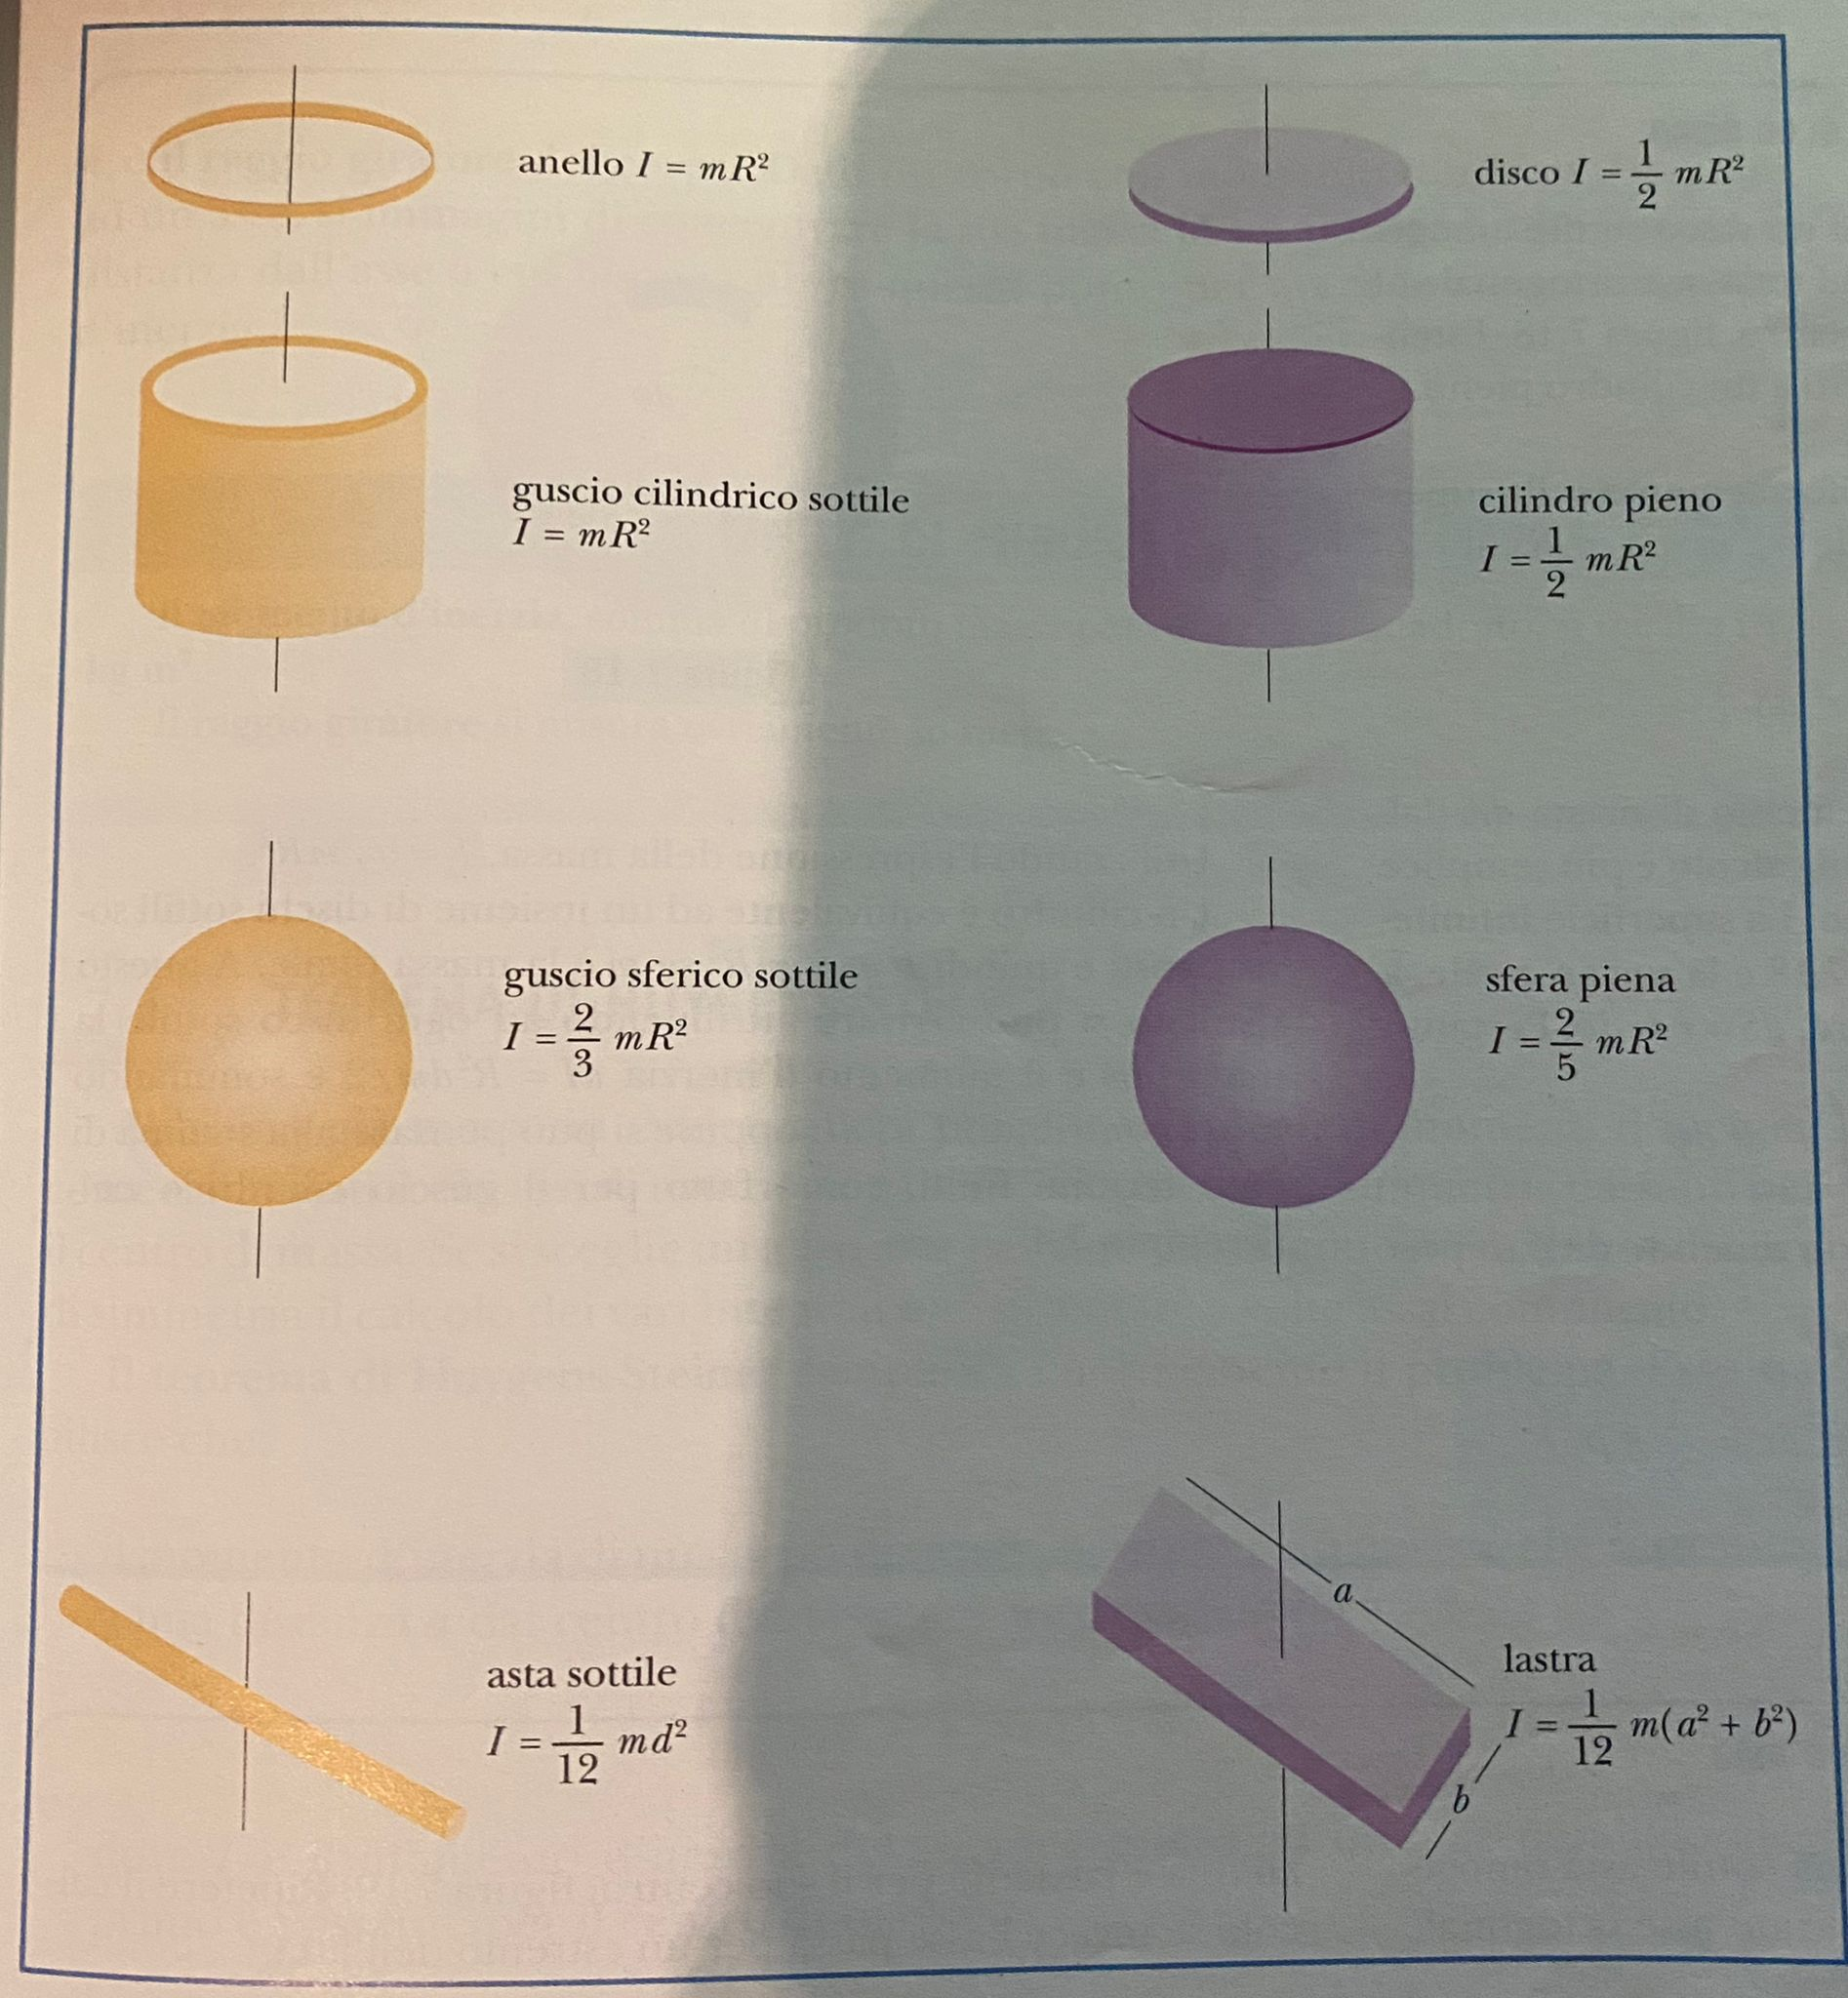
\includegraphics[width=0.7\linewidth]{TabellaMomentoD'Inerzia.jpeg}
    \caption{Tabella dei momenti d'inerzia per i corpi rigidi}
    \label{fig:enter-label}
\end{figure}
\noindent
Ovviamente questa tabella, va imparata a memoria. Notiamo che tutti i corpi rigidi hanno un asse centrale, quest'asse passa per il \textbf{centro di massa} dei corpi. Se i corpi sono omogenei, il centro di massa coincide con i centri di figura. I momenti d'inerzia sono i momenti rispetto a quell'asse di rotazione. Generalmente il \textbf{momento va calcolato rispetto al polo}, il problema però sorge nel momento in cui la tabella sopra ci da le formule, ma rispetto al \textbf{centro di massa}, per questo ci viene in aiuto
\subsection{Teorema di Huygens-Steiner}
Ci aiuta quando vogliamo il momento d'inerzia rispetto ad un altro punto:
\begin{equation}
    I=I_c+md^2
\end{equation}
Dove $I_c$ è il momento d'inerzia rispetto al centro di massa e la d è la distanza tra il centro di massa e il nuovo polo. Infatti questo contributo ci evidenzia come, per far ruotare facilmente l'oggetto questo va fatto ruotare rispetto al suo centro di massa.
\subsection{Piccolo ritorno al momento di una forza}
Nella dinamica abbiamo:
\begin{equation}
    \sum_iF_i=m*a
\end{equation}
Qui abbiamo un problema, mentre il punto di applicazione prima era uno, ora ho diversi punti e quindi ho diversi momenti di conseguenza:
\begin{equation}
    \sum_iM_i=I*\alpha
\end{equation}
Questa legge, vale solamente per due poli che sono: il centro di massa e il punto fisso (che solitamente è quello che preferiamo).
\subsection{Considerazioni energetiche}
Noi sappiamo che $E_m=E_k+E_{pg}+E_{pe}$ l'energia cinetica questa volta va messa in discussione dato che $\frac{1}{2}mv^2$ utilizza una velocità tangenziale, questa volta il corpo oltre che traslare, ruota anche quindi dovremo aggiungere anche un'\textbf{energia cinetica rotazionale}. 
\begin{equation}
    E_{kr}=\frac{1}{2}I\omega^2
\end{equation}
Per quanto riguarda l'\textbf{energia cinetica traslazionale} dobbiamo capire in che punto prendo la velocità, la prenderemo nello stesso punto in cui prendo il momento d'inerzia, la prendo nel centro di massa se non ci sono punti fissi, infatti nei punti fissi $v=0$ e avremo solamente energia cinetica rotazionale. Per quanto riguarda l'\textbf{energia potenziale gravitazionale} h era la quota dal punto materiale rispetto al punto con quota 0. Anche qui abbiamo il problema analogo, ovvero rispetto a quale punto calcolo h? La calcolo rispetto al \textbf{centro di massa}. Un'altro problema di cui ci dobbiamo andare a preoccupare, è il \textbf{lavoro delle forze o dei momenti non conservativi.}
\begin{equation}
    W_M=M*\Delta\theta
\end{equation}
\subsubsection{Centro di massa}
Il centro di massa è quel punto in cui vi è tutta la massa del corpo.
\subsection{Tips per gli esercizi}
Bisogna fare attenzione al calcolo del braccio, e ricordarsi sempre che il libro non sempre ci da direttamente la distanza tra la cerniera e il punto di applicazione della forza. Bisogna ricordarsi che se mi fisso nella cerniera, non c'è energia cinetica traslazionale. Dobbiamo ricordarci la natura rotazionale del problema e che ci sono dei momenti di inerzia che si possono opporre alla rotazione, essendoci momento di inerzia, nel caso in cui abbiamo dei fili, non abbiamo più la situazione ideale in cui il modulo delle tensioni è uguale ma sarà diverso e sarà diversa anche l accelerazione in caso abbiamo dei corpi che possono effettuare delle rotazioni e dei corpi che non possono farlo. Massima attenzione nel fare i disegni. Bisogna ricordarsi per le accelerazioni che la R che prima era il raggio è la distanza rispetto a dove avviene la rotazione.
\section{Lezione 7}
Questa lezione è puramente di esercizi ed è relativa alla \textbf{seconda tipologia di esercizi}. Ci è utile per capire cose che non avevamo detto e come procedere per gli esercizi d'esame.
\subsection{Definizione di Momento}
Non abbiamo mai detto che cos'è il momento di una forza. Ricordiamoci che una \textbf{forza} causa una \textbf{traslazione} e una \textbf{rotazione}. Il \textbf{momento di una forza} misura l'effetto di rotazione che una forza tende a produrre su di un determinato corpo rispetto a un asse. Ricordiamo:
\begin{equation}
    M=\vec{F}*b*sin(\alpha)
\end{equation}
\subsection{Tips per gli esercizi della seconda tipologia}
Gli esercizi che troviamo, generalmente ci parlano di una condizione di equilibrio, in cui \textbf{accelerazione angolare e accelerazione} sono uguali a zero. Questo ci torna utile perchè le equazioni della \textbf{statica} che andiamo a utilizzare sono:
\begin{align}
    & \sum_i\vec{F}=m*\vec{a} \ \ \ \ \xrightarrow[]{} \ \ \ \ \sum_i\vec{F}=0 \\
    & \sum_iM=I*\alpha \ \ \ \ \xrightarrow[]{} \ \ \ \ \sum_iM=0 
\end{align}
Avendo questo tipo di equazioni, ovviamente la prima cosa da fare come per gli esercizi di dinamica è di riportare tutte le forze in gioco. Ci ricordiamo che generalmente i momenti vanno calcolati sullo stesso polo dando priorità ai \textbf{punti fissi} come le cerniere in modo tale che i momenti delle \textbf{reazioni vincolari} si annullino avendo braccio=0. Bisogna quindi fare dei disegni chiari, avere bene in testa quello che sta succedendo, in modo tale da gestire al meglio i segni (i momenti possono andare in senso orario o antiorario) e le equazioni.
\subsubsection{Reazioni Vincolari}
\begin{figure}[H]
    \centering
    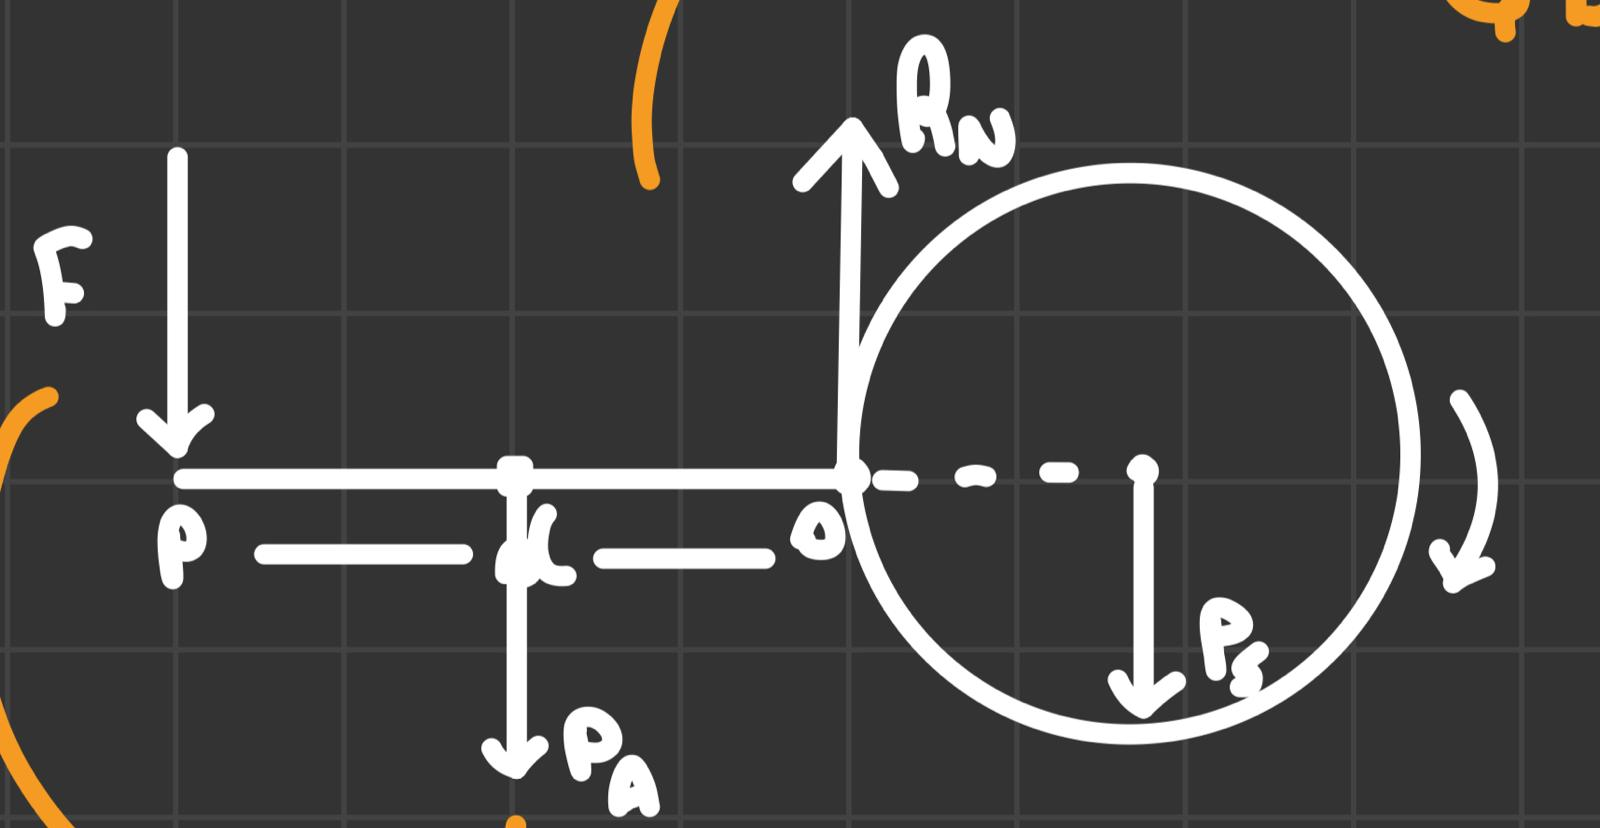
\includegraphics[width=0.5\linewidth]{Mazzoldi7.24.jpg}
    \label{fig:placeholder}
\end{figure}
\noindent
Questo in figura, è l'esercizio 7.24 del Mazzoldi, sono state riportate tutte le forze. Come si può osservare appare una reazione vincolare \textbf{$R_n$}. Ogni qual volta che ho una \textbf{cerniera}, devo considerare due reazioni vincolari, la \textbf{reazione normale} che è \textbf{ortogonale} rispetto al corpo rigido e la \textbf{reazione parallela} la quale è parallela al corpo rigido. Nonostante siamo in presenza di una cerniera nel disegno viene riportata una sola reazione vincolare dato che la seconda, sarebbe stata l'unica sull asse delle x (L'equazione della forza va scalata lungo gli assi) e avremmo avuto sempre utilizzando i metodi di prima:
\begin{equation}
    R_\parallel=0
\end{equation}
Nel caso in cui ho un piano, la reazione vincolare è unica ed è la \textbf{reazione normale}.
\subsection{Continuo dei consigli (inizio esercizi d'esame)}
Molto importante per la stesura dei disegni è ricordare che le forze peso, vanno misurate nel centro di massa che ricordiamo, è quel punto in cui viene applicata tutta la forza peso. Ciò significa che la loro freccia, parte dal centro di massa. Iniziamo considerando l'esercizio del \textbf{16 settembre 2022}. Il disegno iniziale, risulta essere questo:
\begin{figure}[H]
    \centering
    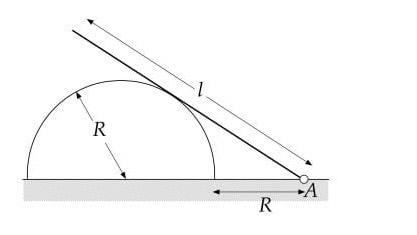
\includegraphics[width=0.5\linewidth]{2esercizio16Settembre2022.jpg}
    \label{fig:placeholder}
\end{figure}
\noindent
Nei problemi della seconda tipologia la manipolazione geometrica è fondamentale. La prima cosa che andiamo a fare è quindi riportare le forze che ci sono in gioco.
\begin{figure}[H]
    \centering
    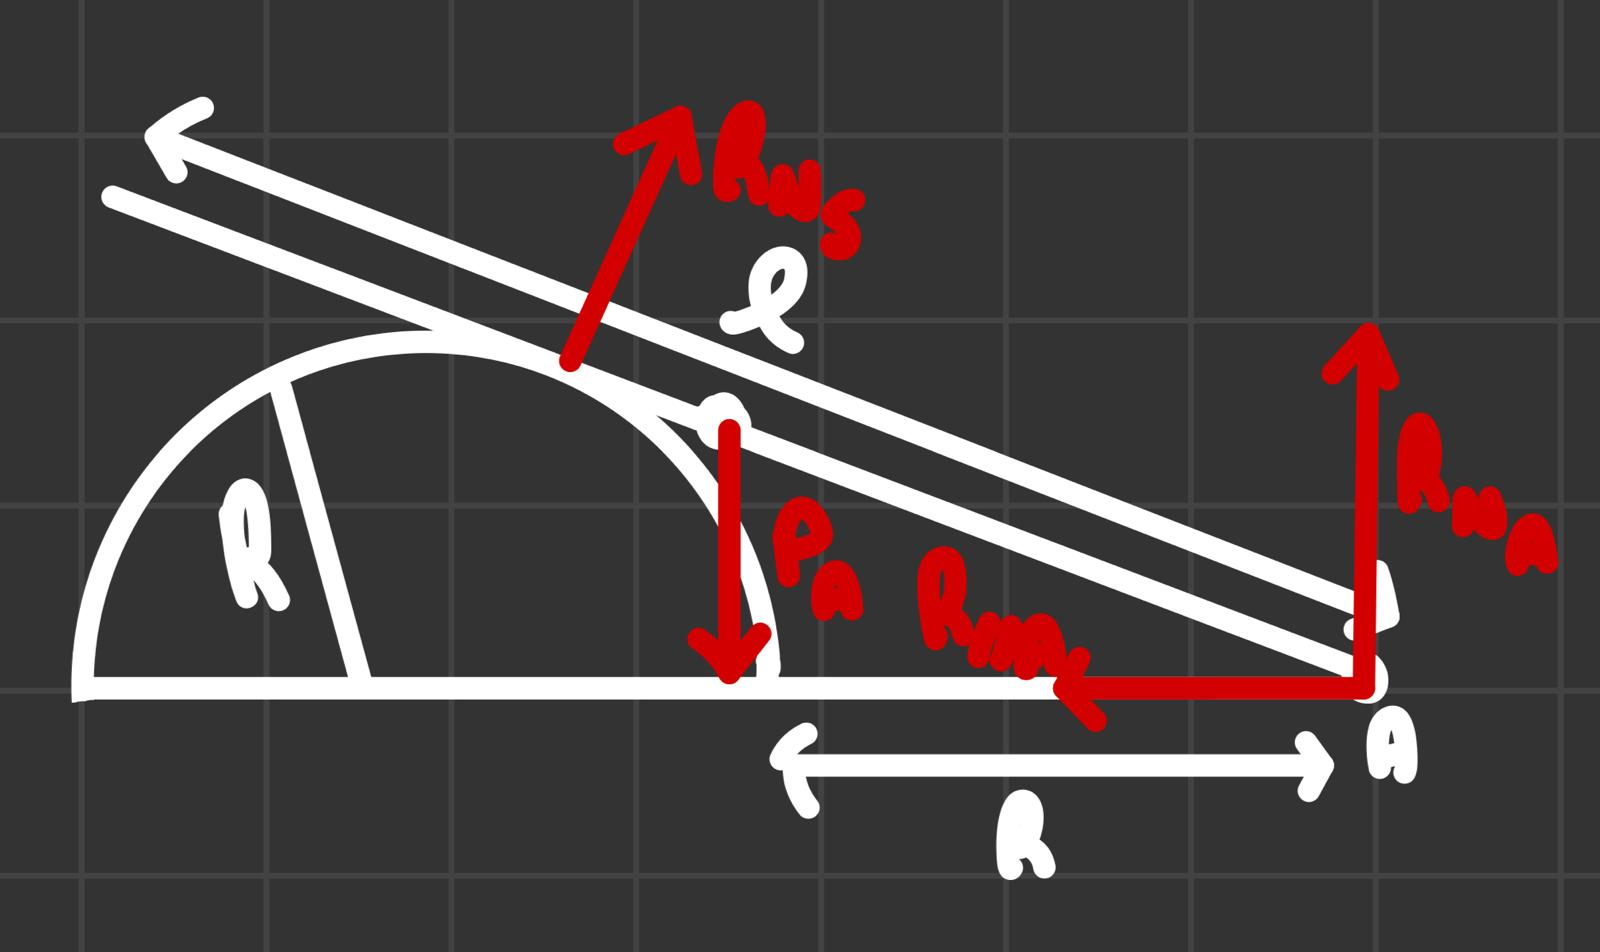
\includegraphics[width=0.5\linewidth]{ForzeInGiocoProblema16settembre2022.jpg}
    \label{fig:placeholder}
\end{figure}
\noindent
Ci sono già da fare delle osservazioni, l'asta non casca grazie alla reazione vincolare del semicilindro, come si vede anche dalla figura, questa è \textbf{ortogonale rispetto all'asta} e non rispetto al piano (è il punto in cui passa una tangente parallela all'asta). Piazzo due assi di riferimento (Anche qui va fatta una precisazione, questi assi vanno orientati in base alle forze, ovvero è \textbf{conveniente usare assi paralleli alle forze in gioco}) e vado a scrivere le equazioni, che ovviamente per quanto riguarda quelle delle forze vanno scalate sugli assi. $R_{na} \ \ e \ \ P_a$ hanno componente totalmente verticale, $R_{ns}$ però ha un inclinazione, ed entrano quindi in gioco degli angoli. Infatti la componente orizzontale sarà data da $R_{ns}cos(\theta)$ e la componente verticale sarà data da $R_{ns}sin(\theta)$.
\begin{figure}[H]
    \centering
    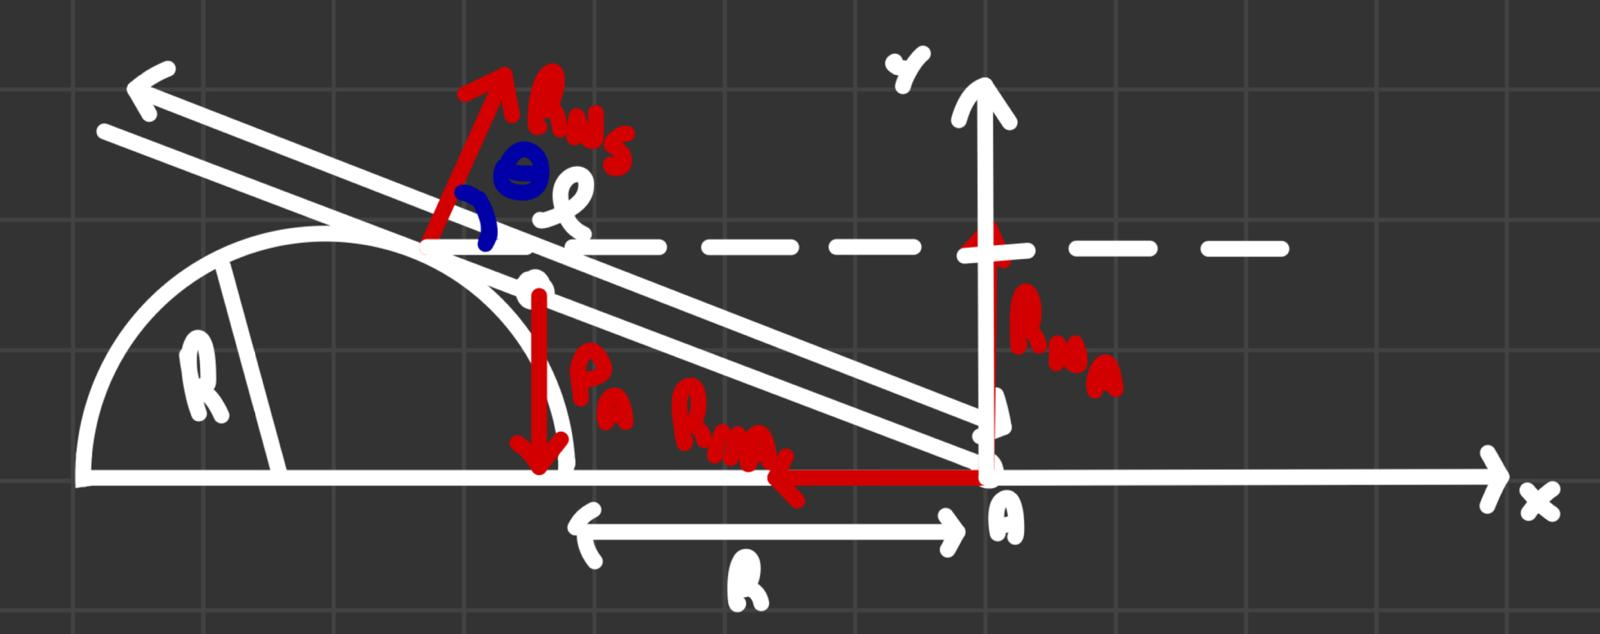
\includegraphics[width=0.5\linewidth]{SecondaFase16settembre2022.jpg}
    \label{fig:placeholder}
\end{figure}
\noindent
Scritte le equazioni relative alla forza scrivo quelle dei momenti. Ovviamente dobbiamo prima \textbf{scegliere il polo}. Scegliamo il polo nella cerniera in modo tale da avere \textbf{nulli i momenti delle reazioni vincolari dell'asta.} Qui vi è da fare una precisazione, in caso di \textbf{equilibrio statico}, tutti i punti sono punti fissi, ciò significa che andiamo a mettere il polo nel \textbf{punto in cui si hanno più reazioni vincolari (in modo da annullarne i momenti)}. Anche qui appaiono, nuovi angoli dato che proprio nella formula del momento abbiamo il \textbf{seno dell'angolo formato tra la direzione del braccio e la direzione della forza.}
\begin{figure}[H]
    \centering
    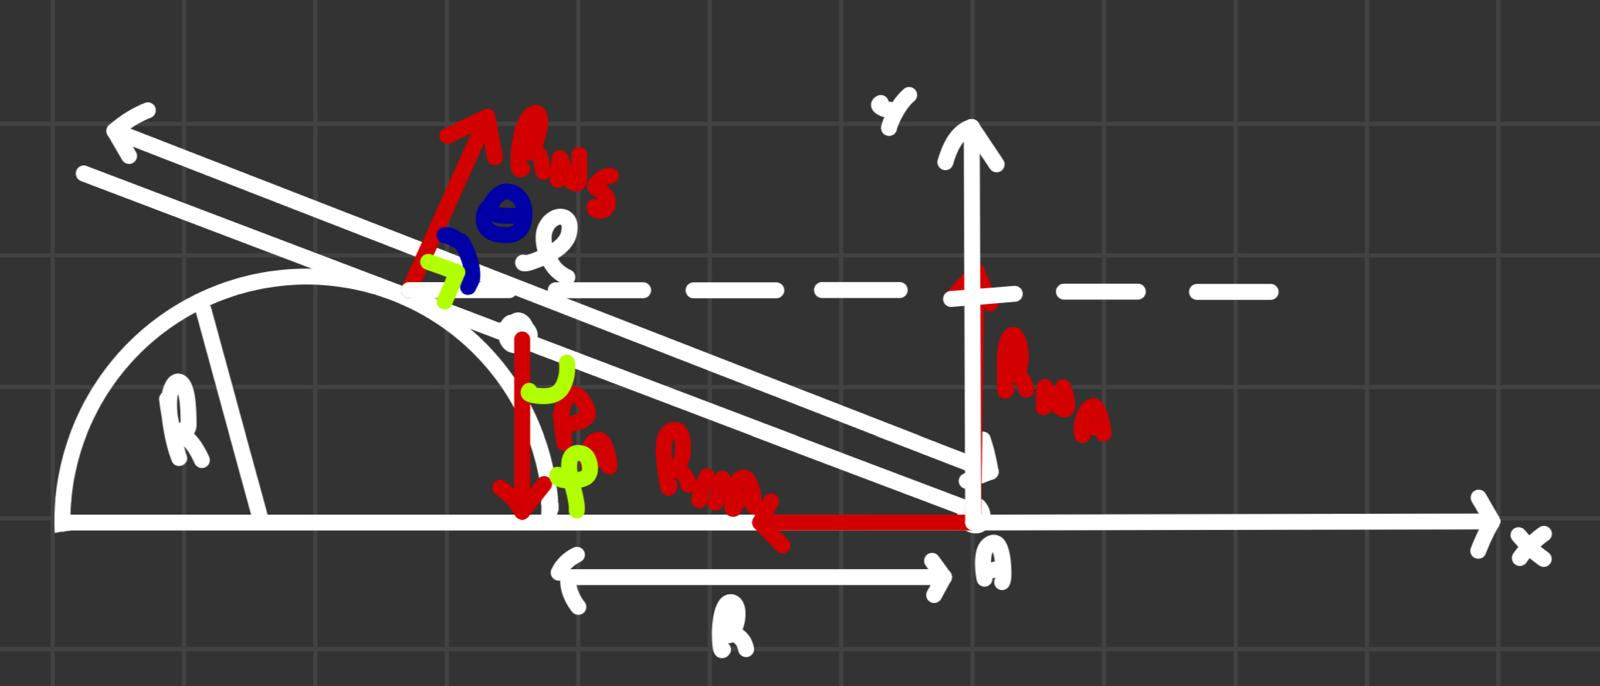
\includegraphics[width=0.5\linewidth]{TerzaFase16settembre2022.jpg}
    \label{fig:placeholder}
\end{figure}
\noindent
L'angolo che forma $R_{ns}$ essendo 90 non viene riportato (questo perche $sin(90)=1$ mentre l'angolo che forma la forza peso invece lo chiamiamo phi. Arriviamo quindi ad avere una situazione di questo tipo:
\begin{figure}[H]
    \centering
    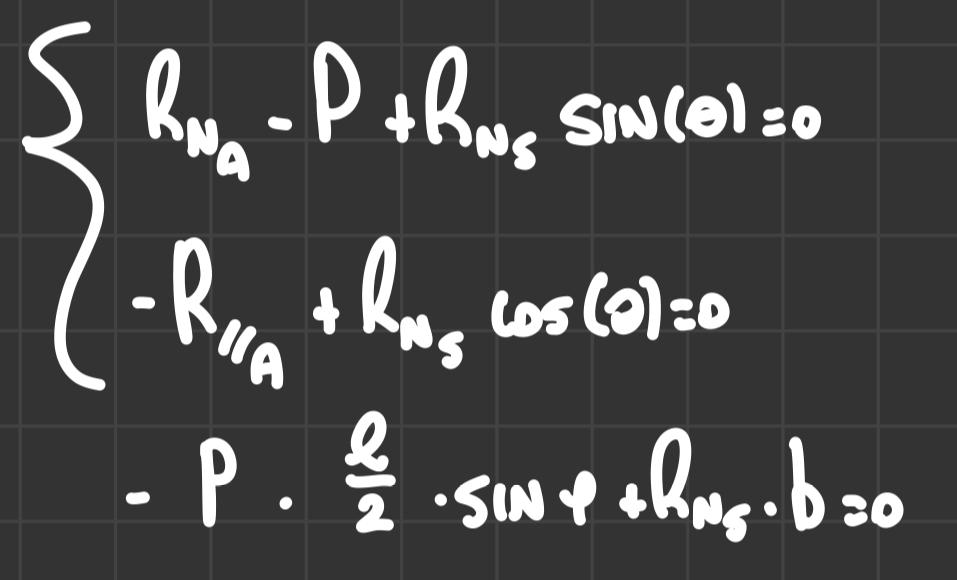
\includegraphics[width=0.5\linewidth]{EquazioniRisolventi16settembre2022.jpg}
    \label{fig:placeholder}
\end{figure}
\noindent
Fin qui i problemi sono quasi tutti uguali, quello che cambia è la \textbf{lavorazione geometrica}, dietro al problema, infatti notiamo come il testo ci chieda le reazioni vincolari, ma nelle equazioni risolutive ci appaiono altre tre incognite, $\theta, b, \phi$. In questo caso si è visto che è conveniente \textbf{dare la priorità ai bracci e a seguire gli angoli}. In questo caso per calcolare il braccio, cerchiamo un triangolo che abbia queste due caratteristiche: \textbf{deve contenere l'incognita e deve contenere gli altri dati che il testo ci ha fornito.}
\begin{figure}[H]
    \centering
    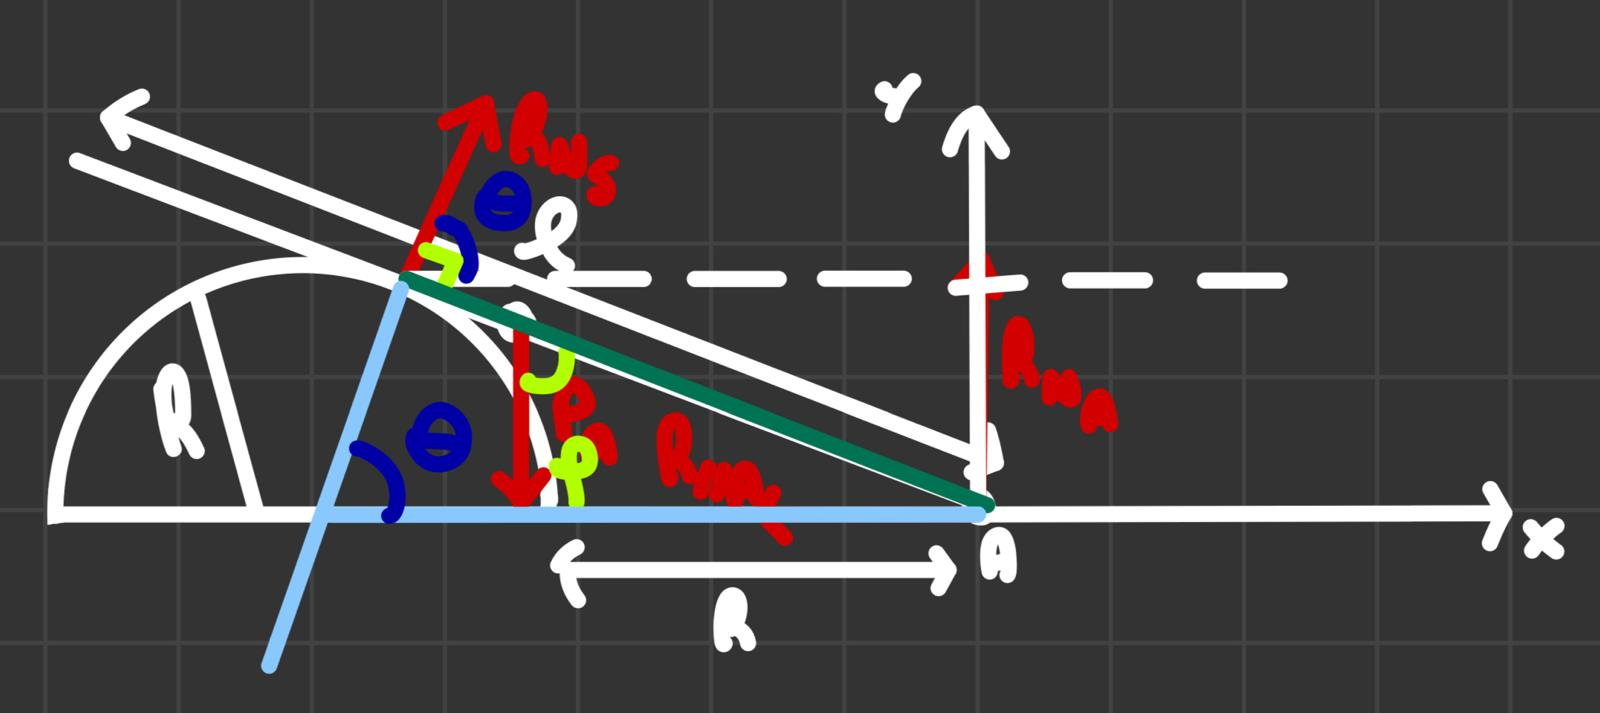
\includegraphics[width=0.5\linewidth]{QuartaFase16settembre2022.jpg}
    \label{fig:placeholder}
\end{figure}
\noindent
In verde scuro il braccio che vogliamo calcolare, in azzurro, il triangolo che utilizzeremo per trovare il braccio. Notiamo infatti che prendendo in considerazione questo triangolo, abbiamo tutti i dati necessari al calcolo del braccio. Il braccio risulta essere la base del triangolo, il raggio del semicilindro la sua altezza e la distanza dal centro del semicilindo alla cerniera la sua ipotenusa, tutti dati che abbiamo nel testo. Calcoliamo il braccio banalmente con pitagora dato che vi è un angolo di 90 gradi. Un'altra osservazione da fare è che questo triangolo ha $\theta$ che possiamo trovare facendo $R=dcos(\theta) \xrightarrow[]{}arccos(\frac{R}{d})=\theta$. Notare come l'angolo non è stato trovato con il seno infatti: \textbf{Se l'angolo è adiacente a R per trovarlo dobbiamo utilizzare il coseno, se l'angolo è opposto dobbiamo utilizzare il seno}. Per trovare phi invece abbiamo due strade, la prima è quella di calcolare l'angolo tutto a destra sapendo che in un triangolo abbiamo che la somma degli angoli è uguale a 180 e rifare la stessa cosa utilizzando l'allungamento di P. Considerando l'angolo viola:
\begin{figure}[H]
    \centering
    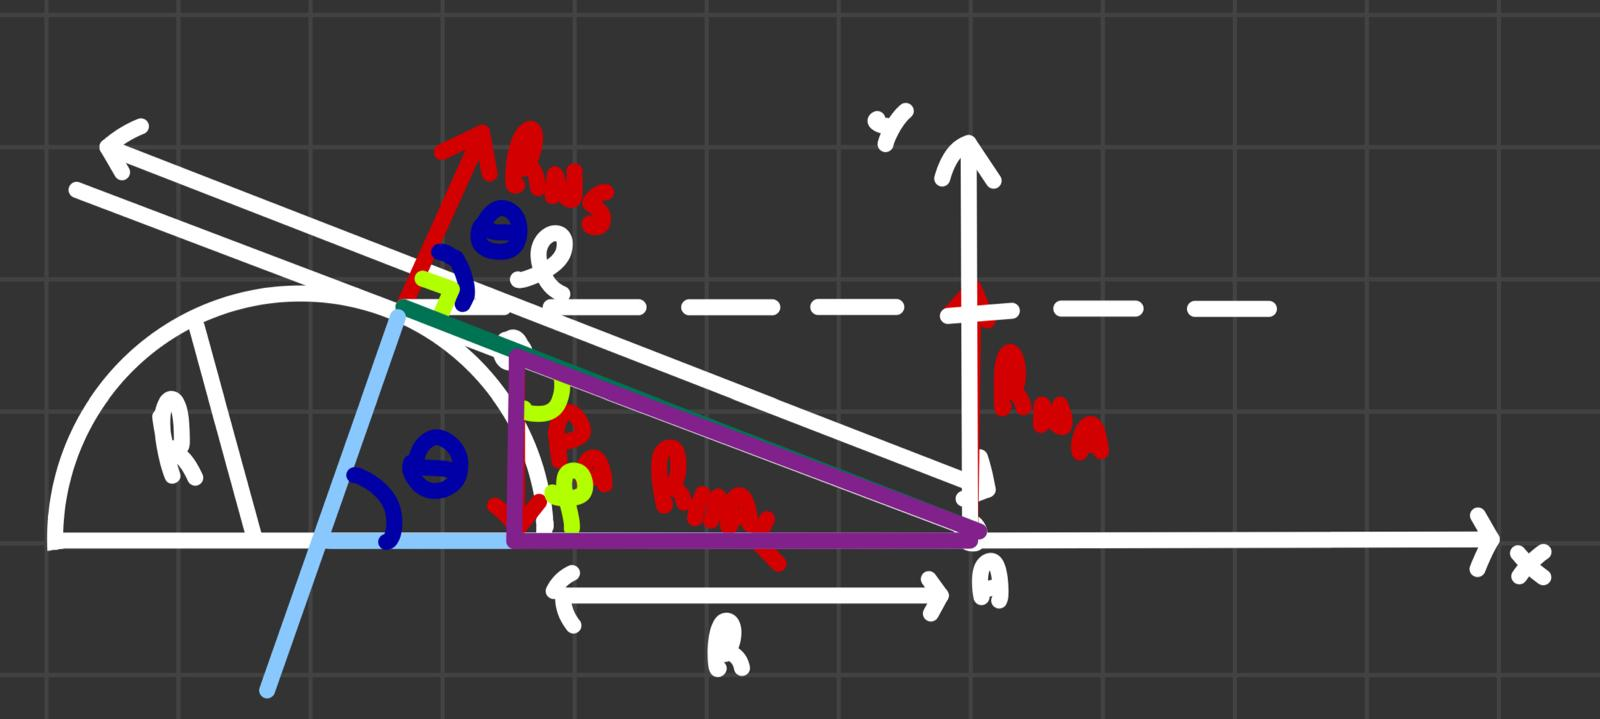
\includegraphics[width=0.5\linewidth]{QuintaFase16Settembre2022.jpg}
    \label{fig:placeholder}
\end{figure}
\noindent
Oppure utilizzando il metodo delle
\subsubsection{Parallele tagliate dalla trasversale}
Utilizzando queste parallele immaginarie che sono sempre o verticali o orizzontali. Dato che \textbf{gli angoli sono a due a due uguali}:
\begin{figure}[H]
    \centering
    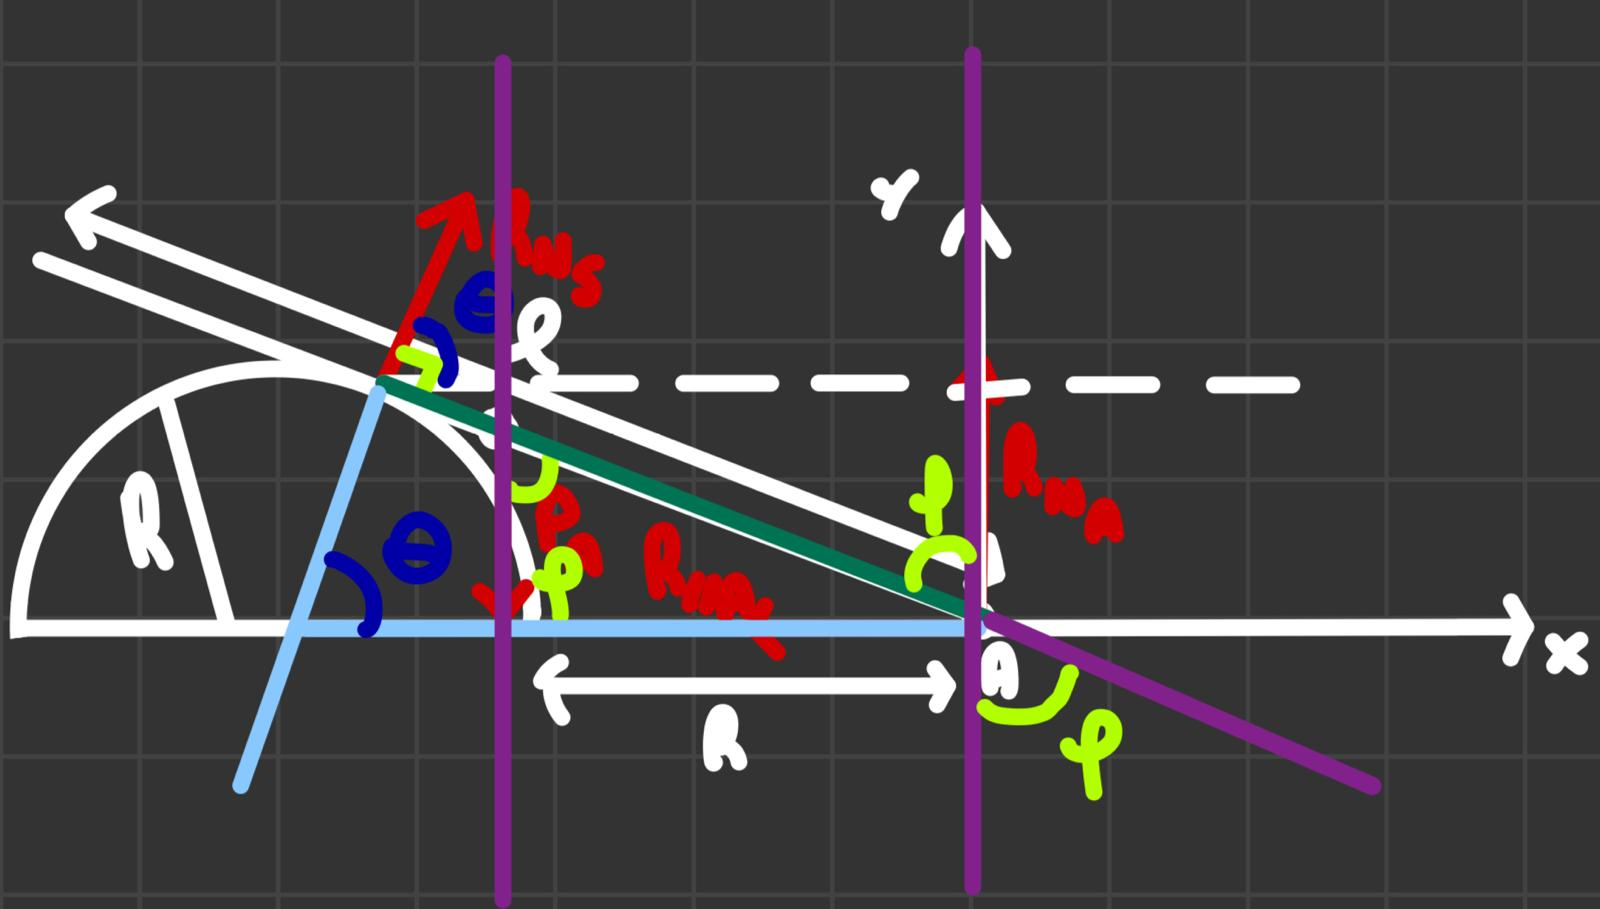
\includegraphics[width=0.5\linewidth]{SestaFase16Settembre2022.jpg}
    \label{fig:placeholder}
\end{figure}
\noindent
Si nota che phi + l'angolo tutto a destra del triangolo trovato prima deve essere 90 gradi e lo si calcola facendo $90-angoloADestra$. In questo modo ho trovato le tre incognite aggiuntive, ora risolvo un semplice sistema di tre equazioni e tre incognite.
\subsubsection{Esercizio dell'ombrello chiuso poggiato su un piano (introduzione)}
Ricordiamo che quando dice \textbf{equilibrio} significa che dobbiamo usare le equazioni della statica, forze e momenti. Ricordiamo che un \textbf{asse di simmetria è un asse che divide la figura in 2 parti uguali}. Questo esercizio va continuato. Ricordiamo inoltre che parliamo di \textbf{reazione vincolare} quando un corpo è soggetto a un vincolo (cioè una condizione che limita i suoi possibili movimenti) e il vincolo esercita sul corpo una \textbf{forza di reazione} per far rispettare quella condizione.
\newpage
\section{Lezione 8}
\subsection{Esercizio dell'ombrello chiuso poggiato su un piano}
Continuiamo con gli esercizi, in modo tale da capire al meglio come affrontare la seconda tipologia. Come tutti i problemi, la prima cosa che bisogna fare è disegnare tutte le forze in gioco:
\begin{figure}[H]
    \centering
    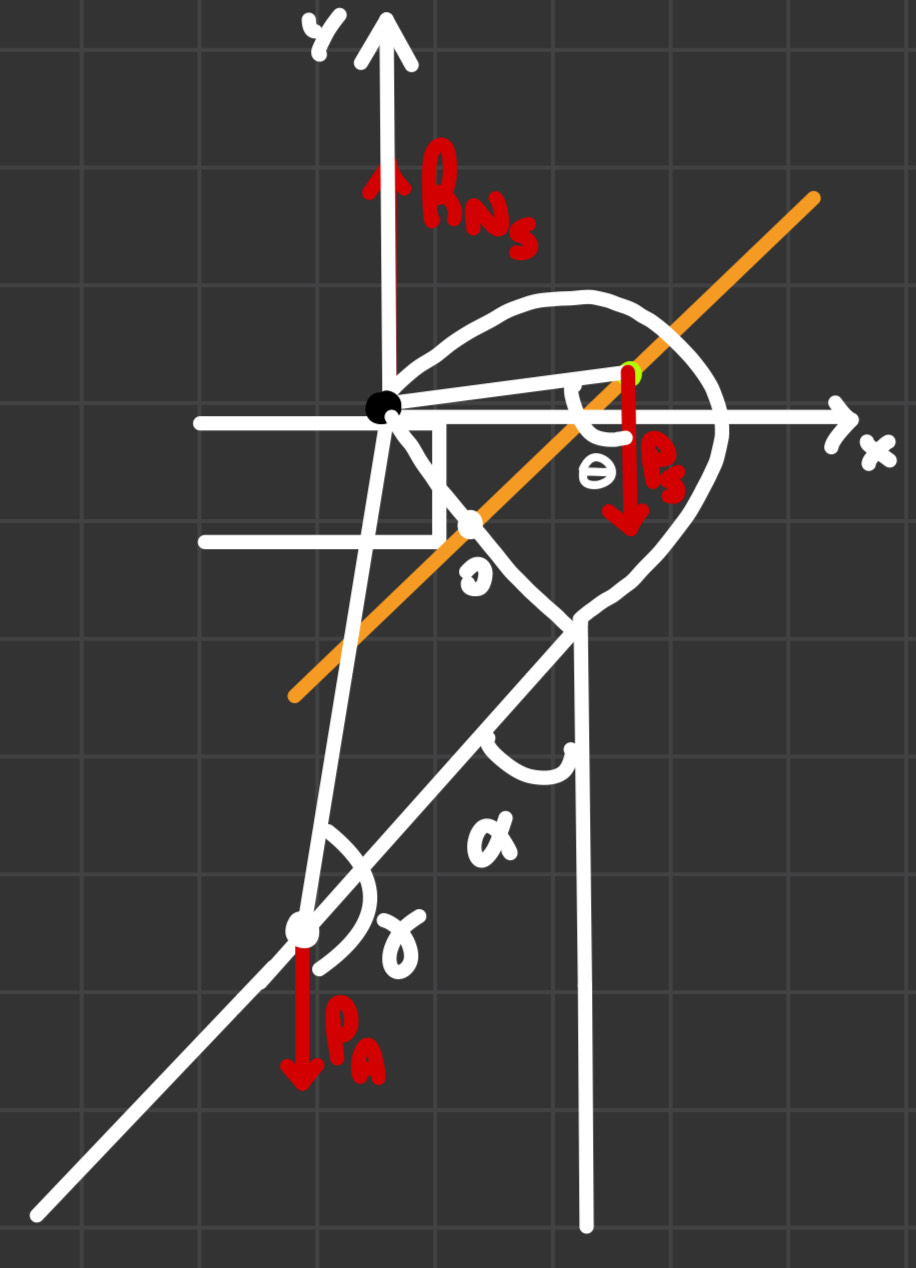
\includegraphics[width=0.3\linewidth]{PrimaFaseProblemaDellOmbrello.jpeg}
    \label{fig:placeholder}
\end{figure}
\noindent
Come si vede dalla figura scrivo l'equazione delle forze e successivamente quella dei momenti. In quella dei momenti, appariranno i bracci. I bracci non sono altro che le distanze, per questo per trovarli mi basta tracciare dei segmenti, come già fatto in figura. 
\subsubsection{Regola generale per capire la rotazione dei momenti}
Per capire la rotazione seguiamo tre semplici step: il \textbf{primo} in cui disegno il braccio, il \textbf{secondo} in cui prendo una penna (da dietro) e "simulo" il braccio, il \textbf{terzo} step è quello più importante perche andiamo a tirare giù la penna con la forza peso, ovvero spingo la punta verso il basso, quindi dove ruota la penna sarà la direzione del momento.
\subsubsection{Osservazioni sul sistema di equazioni}
Si può notare come anche questa volta sono presenti delle incognite ausiliari, i bracci, la reazione vincolare del piano sul semianello e gli angoli. Come possiamo notare in questo caso abbiamo 4 incognite di natura geometrica, il braccio della forza peso del semianello, il braccio della forza peso dell'asta e gli angoli da loro formati (trovato con il metodo della penna). La restante incognita è la reazione vincolare, solitamente il testo richiede le reazioni vincolari ma non in questo caso, inoltre un'incognita geometrica ideologicamente potrebbe esser trovata anche risolvendo il sistema di equazioni essendo formato da due equazioni. L'ultima osservazione è che nel testo ci chiede $\alpha$ che non sembra neanche apparire nelle equazioni, quando parliamo di \textbf{equilibrio} queste sono le equazioni risolventi e per questo motivo dovremo far apparire qui alpha.
\subsubsection{Ricerca dei bracci}
Come è emerso dagli altri esercizi, è chiaro che il metodo da la priorità ai bracci e lo fa \textbf{cercando dei triangoli rettangoli che li contengano}. Individuiamo per il braccio b1 il triangolo in azzurro:
\begin{figure}[H]
    \centering
    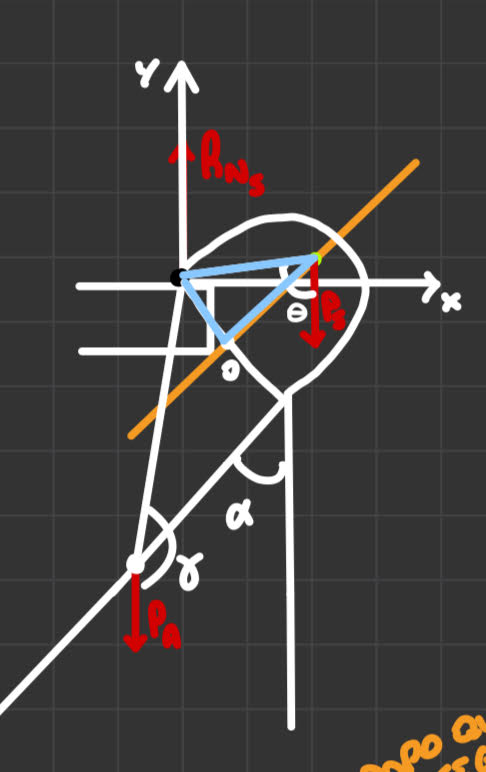
\includegraphics[width=0.3\linewidth]{SecondaFaseOmbrello.jpg}
    \label{fig:placeholder}
\end{figure}
\noindent
La distanza dal centro o al centro di massa del semianello è fornita dal testo, il raggio ce lo da il testo, riesco facilmente a trovare il braccio con pitagora. Per l'altro braccio, il discorso è analogo, lo ho addirittura già evidenziato nel disegno, in blu scuro:
\begin{figure}[H]
    \centering
    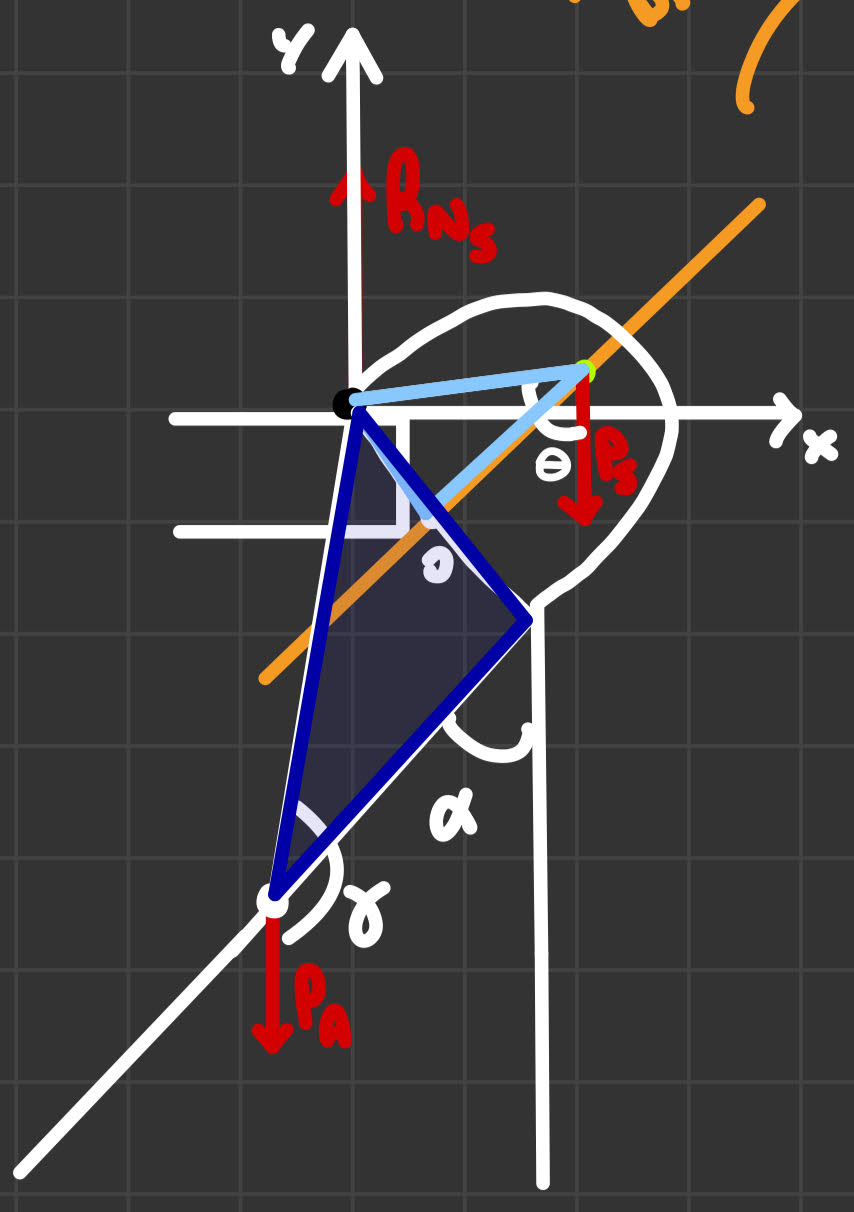
\includegraphics[width=0.27
    \linewidth]{TerzaFaseOmbrello.jpg}
    \label{fig:placeholder}
\end{figure}
\noindent
\subsubsection{Ricerca degli angoli e risoluzione finale}
Normalmente quello che vogliamo, è che gli angoli si trovino all'interno dei triangoli che abbiamo già trovato, per troverli facilmente con la trigonometria. Qui abbiamo che entrambi gli angoli, si ritrovano a essere partizionati dai nostri triangoli. Iniziamo con theta, chiameremo l'angolo sopra $\theta'$ e quello sotto $\theta''$. $\theta'$ si trova facilmente con la trigonometria, stesso discorso per $\gamma '$. Adesso un'altra cosa molto standard è quella di \textbf{tracciare le direzioni dell'angolo e trovare relazioni con i nostri angoli}. Ricordiamo due angoli sono a due a due uguali quando le direzioni che formano l'angolo sono a due a due parallele o ruotate dello stesso angolo. Un'angolo infatti è formato da due direzioni. Ci accorgiamo infatti che $\theta''$ non è altro che $\alpha$ l'incognita dell'esercizio. Ora quindi dobbiamo capire come trovarlo.
\begin{figure}[H]
    \centering
    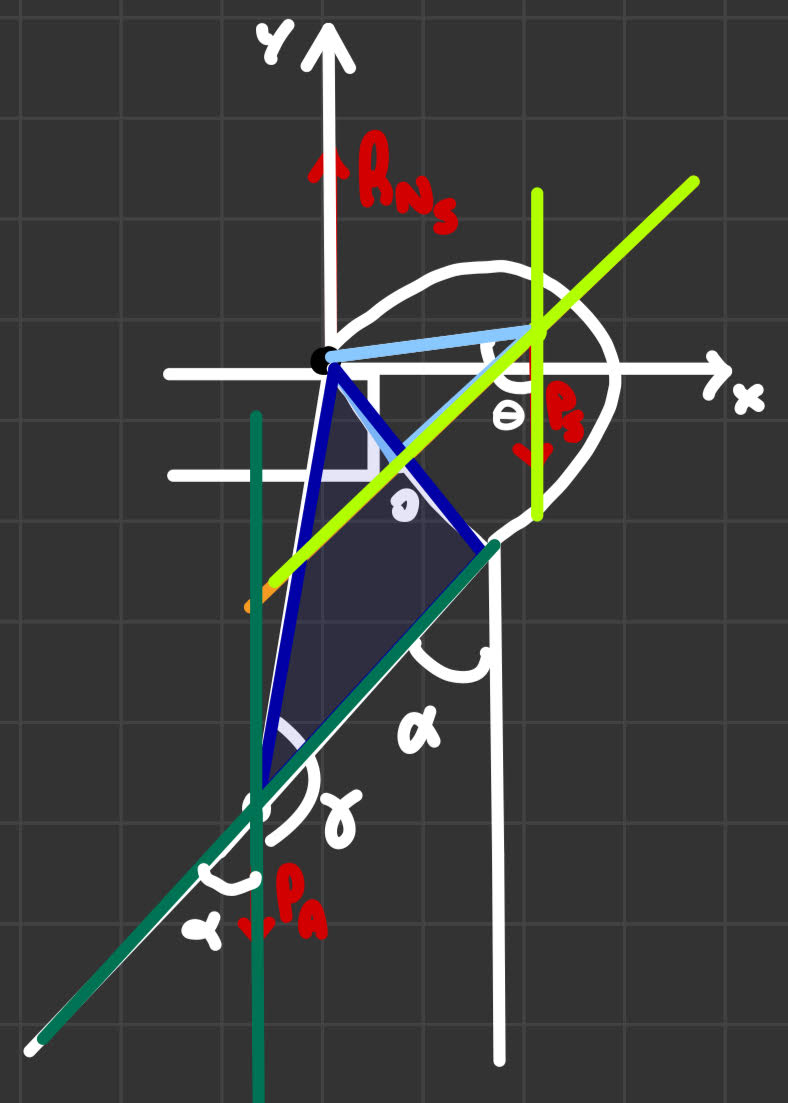
\includegraphics[width=0.3\linewidth]{QUartaFaseOmbrello.jpg}
    \label{fig:placeholder}
\end{figure}
\noindent
Osserviamo che vi è una relazione tra $\alpha \ \ e \ \ \gamma''$ infatti $\gamma''=180-\alpha$ e quindi $\gamma=\gamma'+180-\alpha$ inoltre $\theta=\theta'+\alpha$, sostituiamo i dati nell'equazione e la risolviamo, in modo tale da trovare l'incognita.
\subsection{Problema delle due aste saldate}
Vediamo ora il problema delle due aste saldate che ha una risoluzione analoga a quelle viste in precedenza. Disegno le forze, individuo i bracci e gli angoli:
\begin{figure}[H]
    \centering
    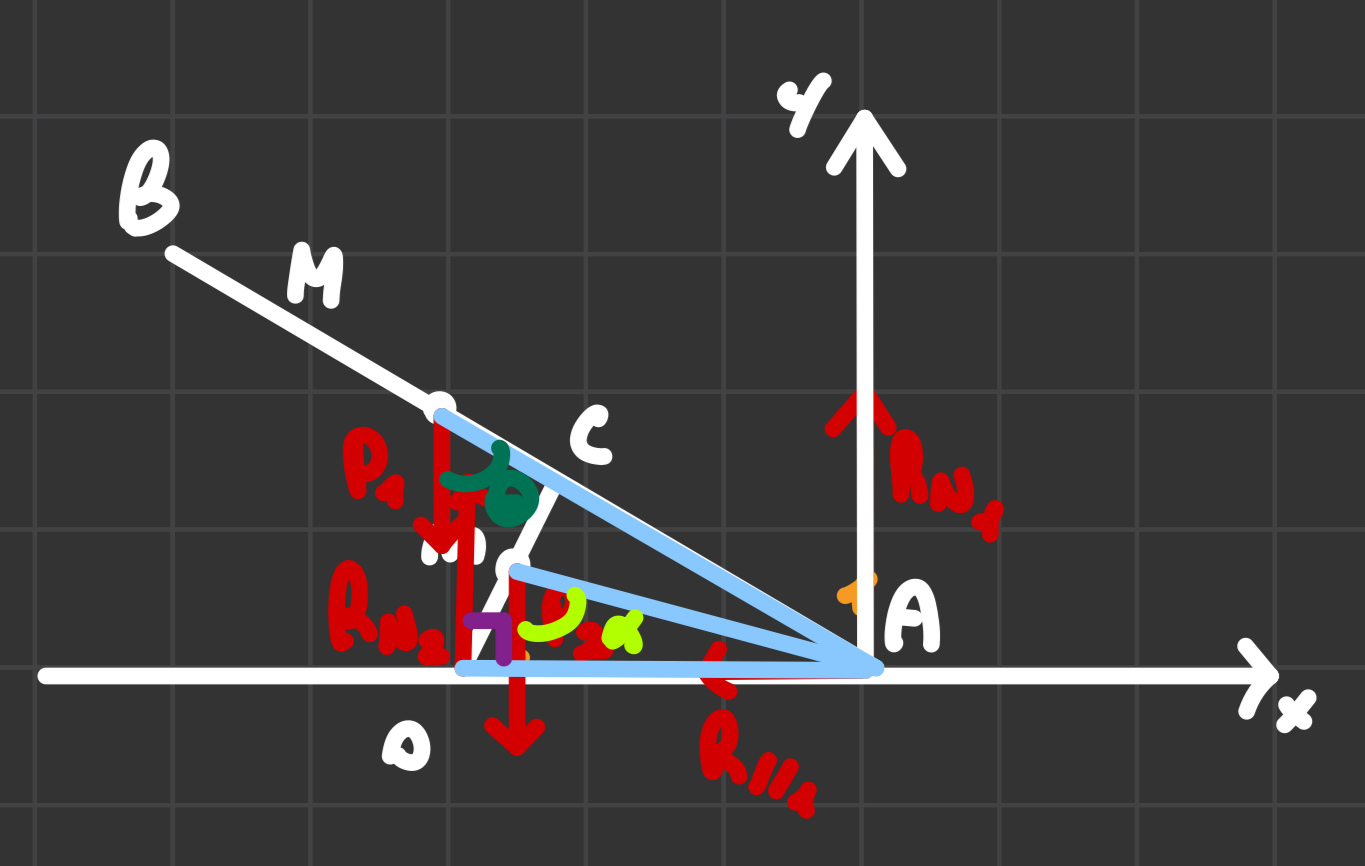
\includegraphics[width=0.3\linewidth]{PrimaFaseAste.jpg}
    \label{fig:placeholder}
\end{figure}
\noindent
Un'osservazione, il sistema in equilibrio, è da considerare come un'unico corpo. Come tutti gli altri problemi, segue la formulazione solita per la risoluzione.
\subsubsection{Ricerca dei bracci}
Il braccio 1 è in realtà noto e corrisponde al centro delle masse dell'asta grande. Il terzo braccio, lo troviamo con il triangolo in viola:
\begin{figure}[H]
    \centering
    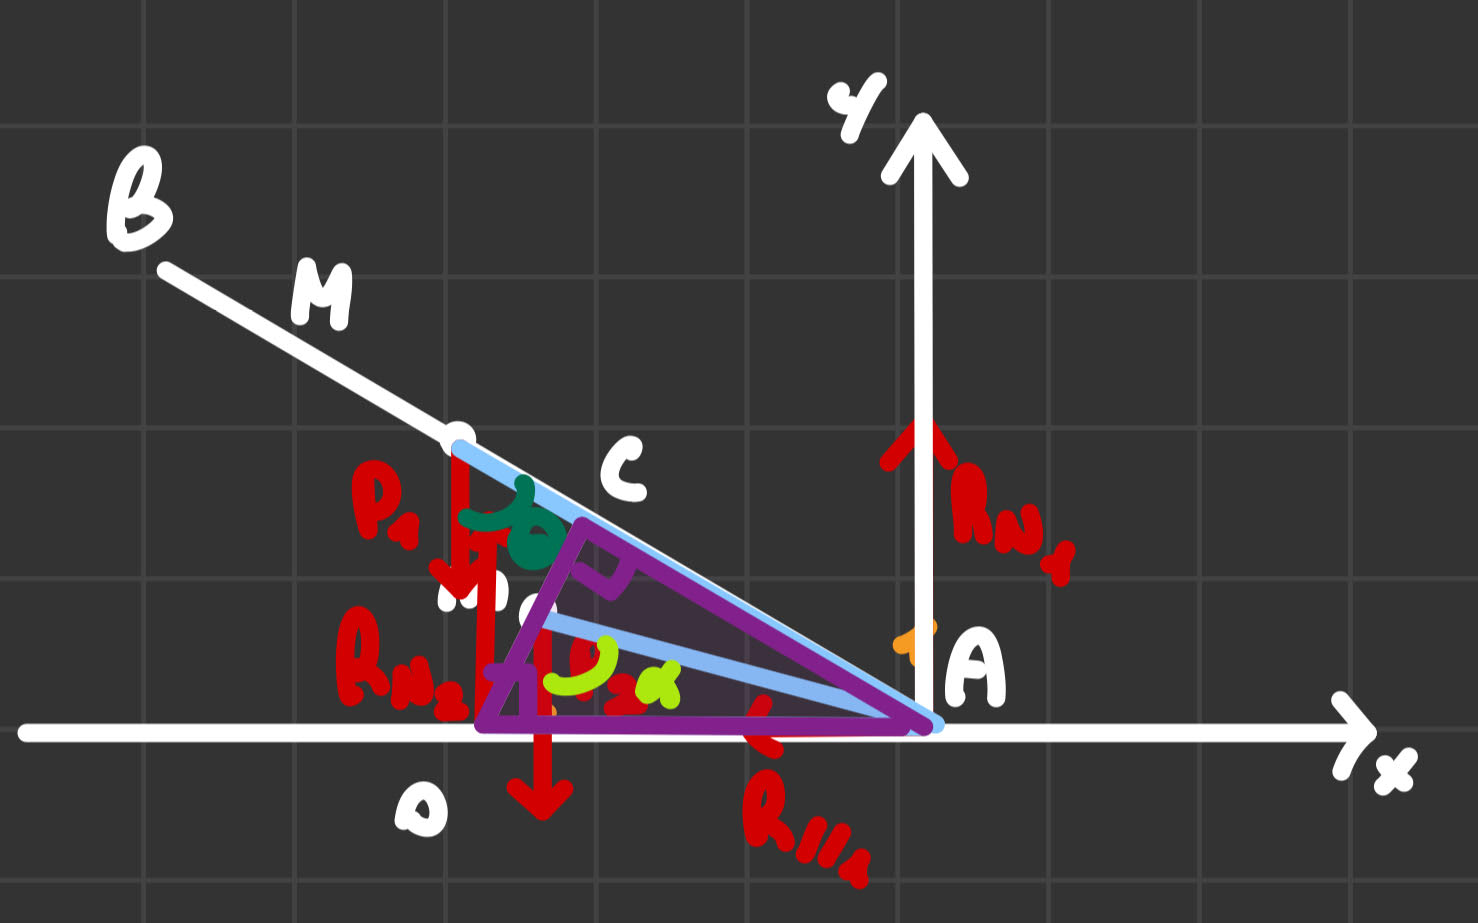
\includegraphics[width=0.4\linewidth]{SecondaFaseAste.jpg}
    \label{fig:placeholder}
\end{figure}
\noindent
Resta quindi da trovare il braccio 2, che troviamo con il triangolo in verde scuro.
\begin{figure}[H]
    \centering
    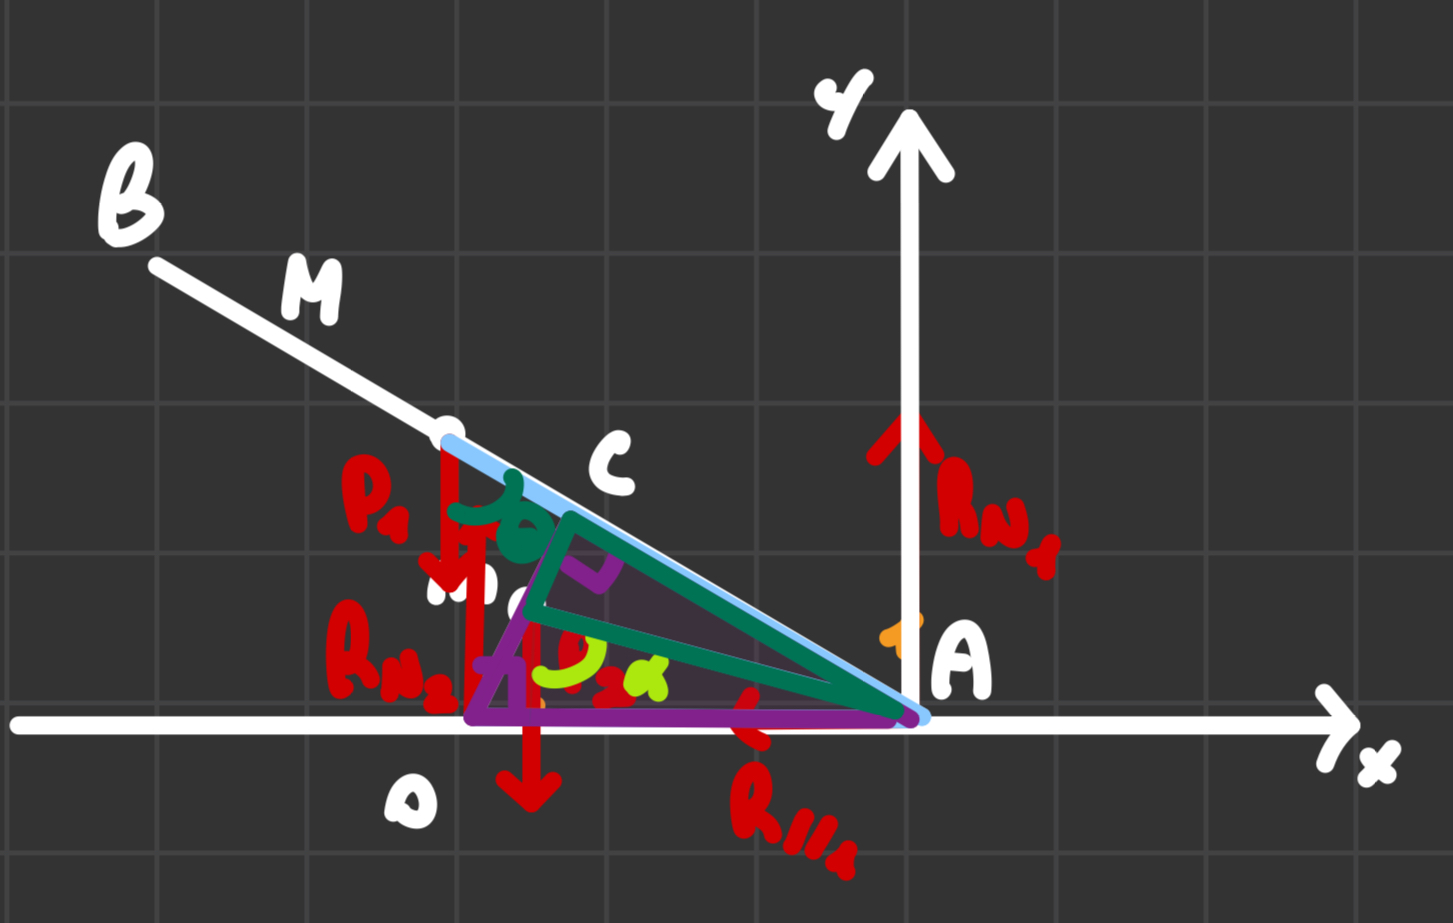
\includegraphics[width=0.4\linewidth]{TerzaFaseAste.jpg}
    \label{fig:placeholder}
\end{figure}
\noindent
\subsubsection{Ricerca degli angoli e risoluzione del problema}
Trovo $\theta$ osservando il triangolo bianco che troviamo con l'allungamento di P1.
\begin{figure}[H]
    \centering
    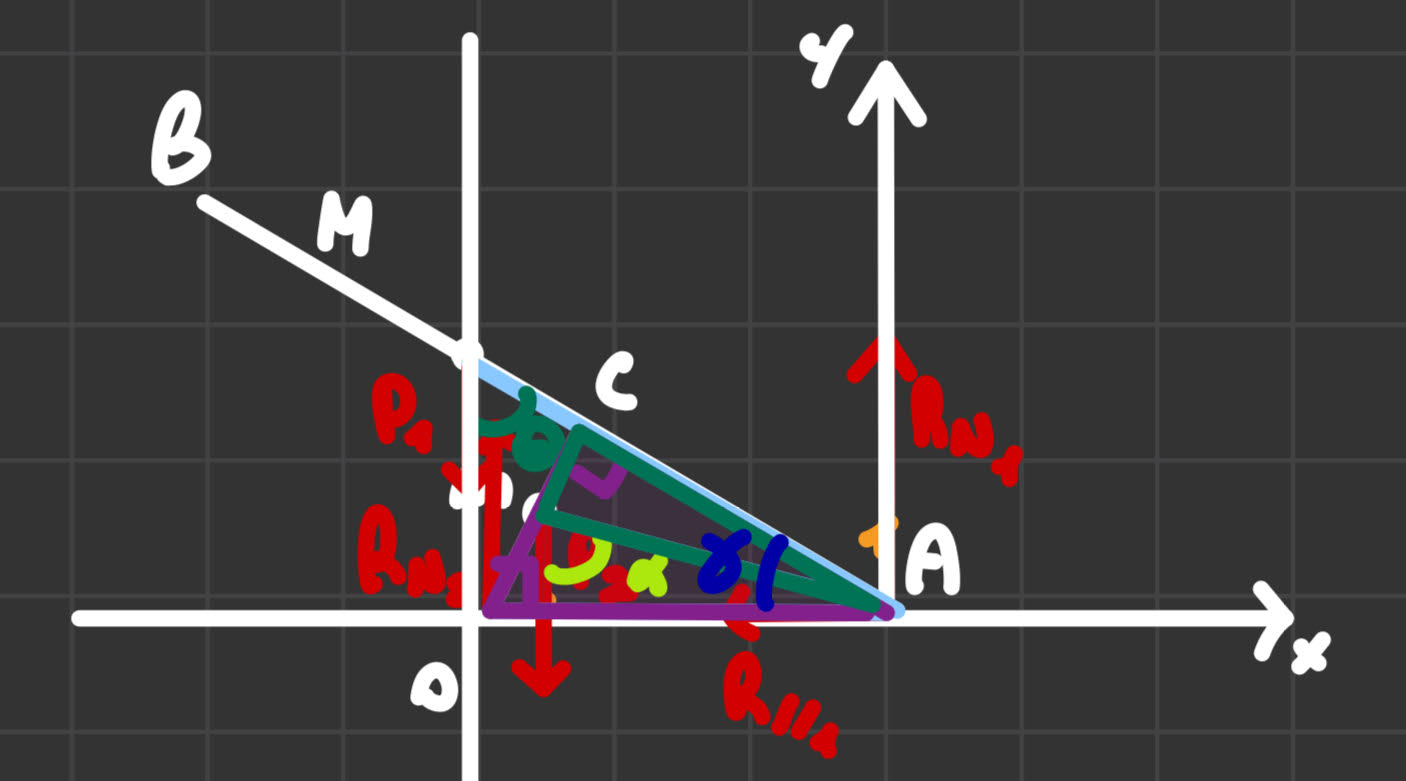
\includegraphics[width=0.4\linewidth]{QuartaFaseAste.jpg}
    \label{fig:placeholder}
\end{figure}
\noindent
Infatti capisco che $\theta=180-90-\gamma$. Siccome $\gamma$ si trova anche nel triangolo viola che avevamo precedentemente utilizzato me lo calcolo e calcolo successivamente $\theta$. Dunque mi resta da trovare l'ultimo angolo, $\alpha$. Evidenzio il triangolo in blu:
\begin{figure}[H]
    \centering
    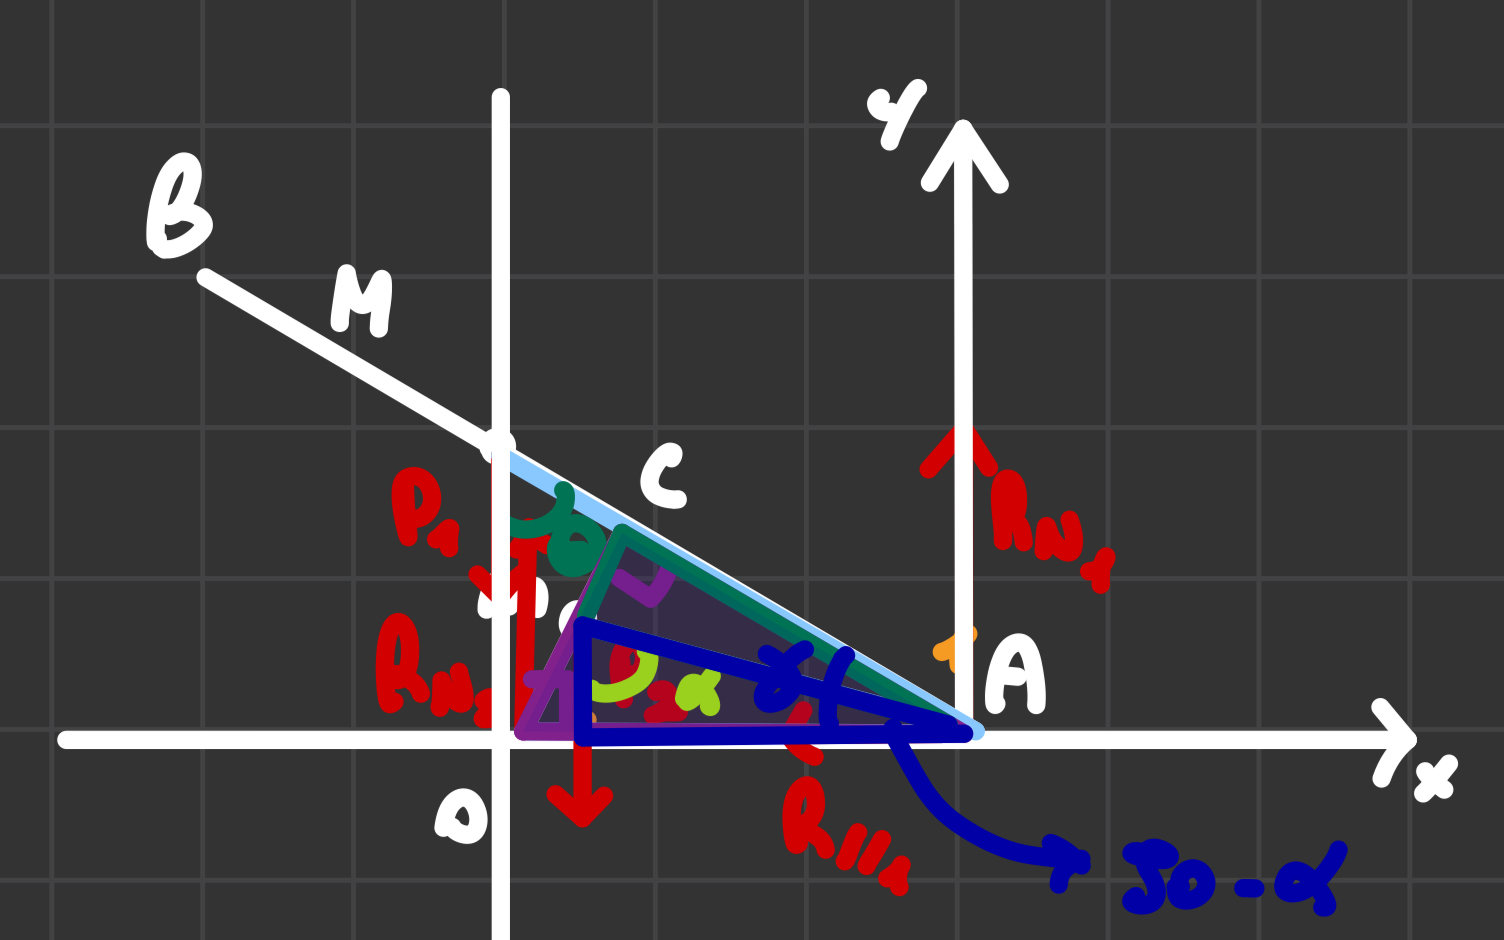
\includegraphics[width=0.4\linewidth]{QuintaFaseAste.jpg}
    \label{fig:placeholder}
\end{figure}
\noindent
Anche questa volta abbiamo un angolo partizionato ed è proprio $\gamma$. Notiamo infatti che $\alpha=180-90-\gamma''$. $\gamma$ già lo conosciamo, dunque è necessario trovarne solo una parte. Il primo triangolo verde scuro che abbiamo utilizzato contiene proprio $\gamma'$, lo calcolo con la trigonometria e calcolo facilmente $\gamma''=\gamma-\gamma'$, successivamente calcolo $\alpha$. Notare come si poteva usare anche il metodo delle direzioni degli angoli: 
\begin{figure}[H]
    \centering
    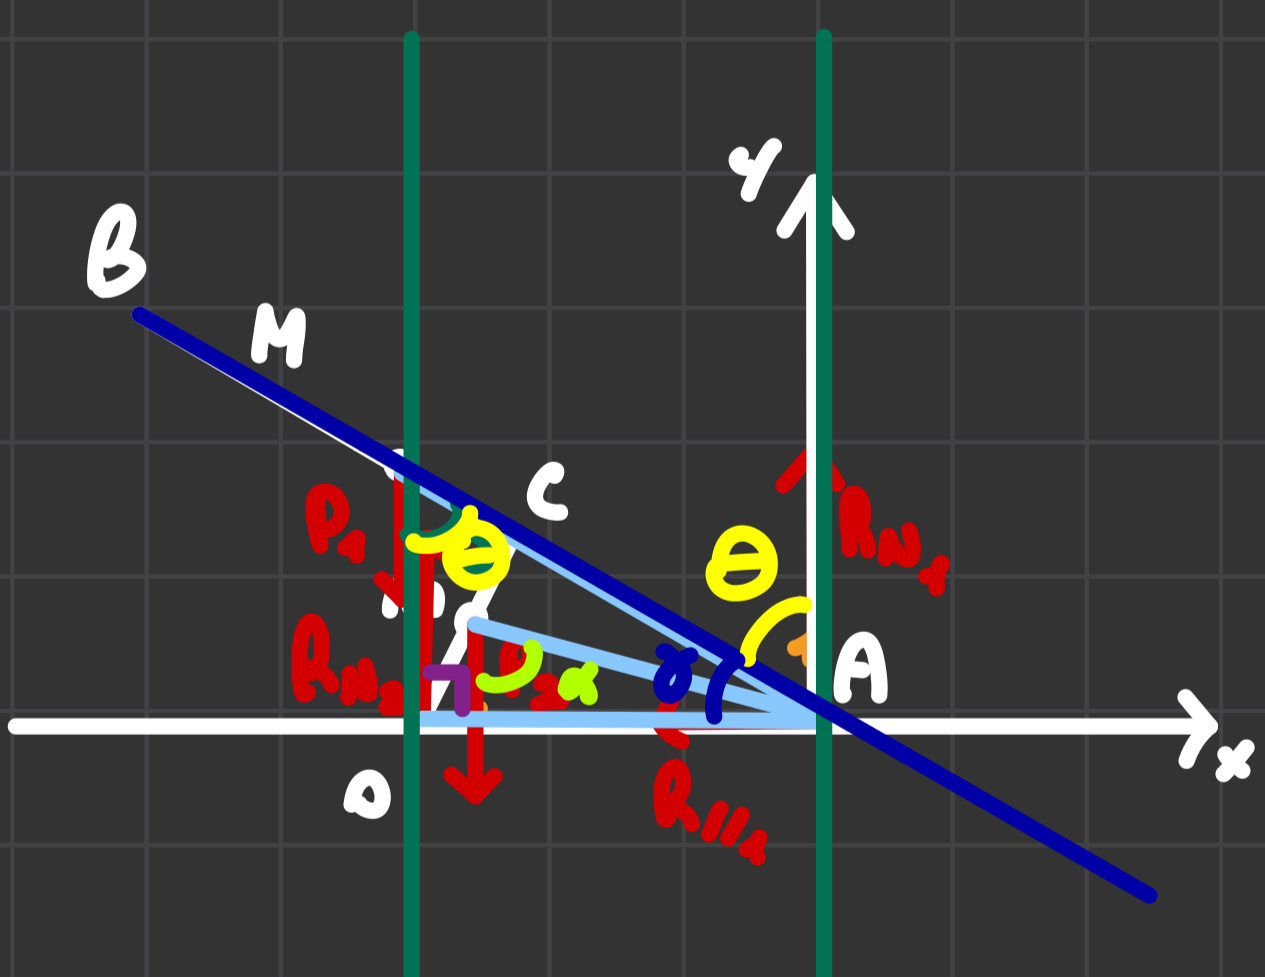
\includegraphics[width=0.4\linewidth]{SestaFaseAste.jpg}
    \label{fig:placeholder}
\end{figure}
\noindent
Stabilendo che $\theta-\gamma=90$. Risolvo il sistema con tutti i dati e trovo il rapporto delle masse.
\section{Lezione 9}
Anche questa lezione riguarda solamente esercizi, in particolare, capiamo come trovare la velocità angolare nel caso dei corpi rigidi. Inoltre la prossima sarà l'ultima lezione in cui andremo a introdurre come lavorare in caso di piccole oscillazioni e di attrito.
\subsection{Ricerca della velocità angolare}
Per trovare la velocità angolare, utilizzeremo il \textbf{metodo energetico}. Potrei pensare di calcolarla con la cinematica, ma queto non conviene perchè non ho il tempo, potrei uscirne con la posizione, ma questo continua a non valere dato che queste leggi valgono solo nei casi in cui l'\textbf{accelerazione è costante}. In questo caso $\alpha$ non è costante. Nell'esercizio che sto considerando, se tolgo l'asta piccola, avrò solamente la forza peso che spingerà in basso l'asta grande. Ideologicamente noi vorremmo un accelerazione costante e quindi i momenti costanti, cosa che però non riusciamo a avere, dato che P e b non cambiano, quello che cambia è \textbf{l'angolo che sarà in funzione del tempo}. Per cui il metodo energetico ci piace perchè tutte le forze degli esercizi generalmente sono conservative. Infatti vorremmo che i lavori delle forze non conservative siano pari a 0 ed è quello che succede in questi casi, abbiamo quindi $E_{mi}=E_{mf}$. Va specificato inoltre che ci sarebbero le reazioni vincolari che sono forze non conservative, che però stando sui punti fermi hanno lavoro nullo.
\subsubsection{Risoluzione seconda parte delle due aste}
Nota: sul metodo energetico, per quanto riguarda i corpi rigidi, \textbf{l'energia cinetica che consideriamo è puramente rotazionale}, questo perche consideriamo tutti i punti dato che tutti i punti effettuano una rotazione rispetto alla cerniera. Non c'è molto altro da dire su quest'esercizio, dato che il proseguimento è puramente matematico.
\subsection{Problema dell'asta e dell'anello}
\begin{figure}[H]
    \centering
    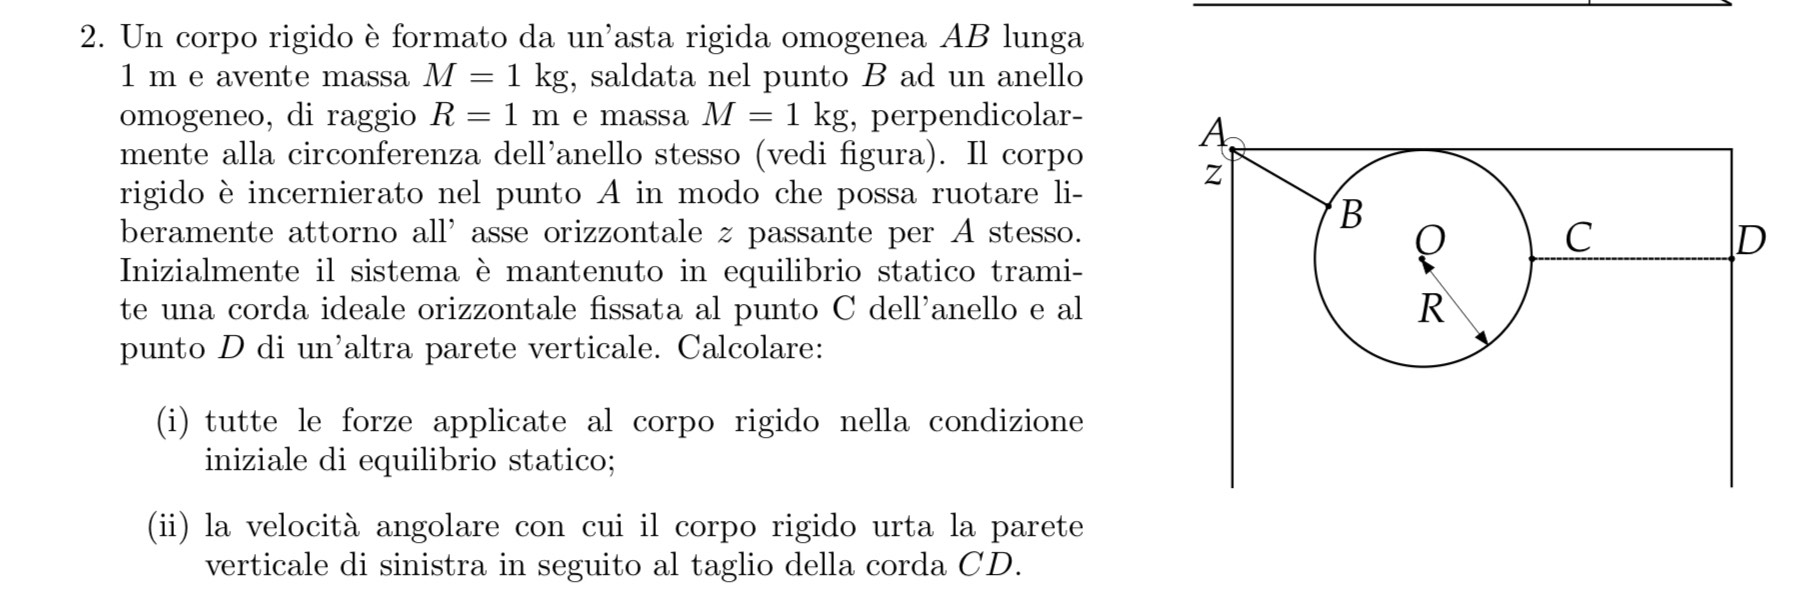
\includegraphics[width=0.8\linewidth]{ProblemaDellAstaEDellAnello.jpeg}
    \label{fig:placeholder}
\end{figure}
\noindent
Ricordiamo, una corda ideale è una corda senza massa. Come al solito, individuo le forze i bracci e gli angoli e determino il sistema di equazioni.
\begin{figure}[H]
    \centering
    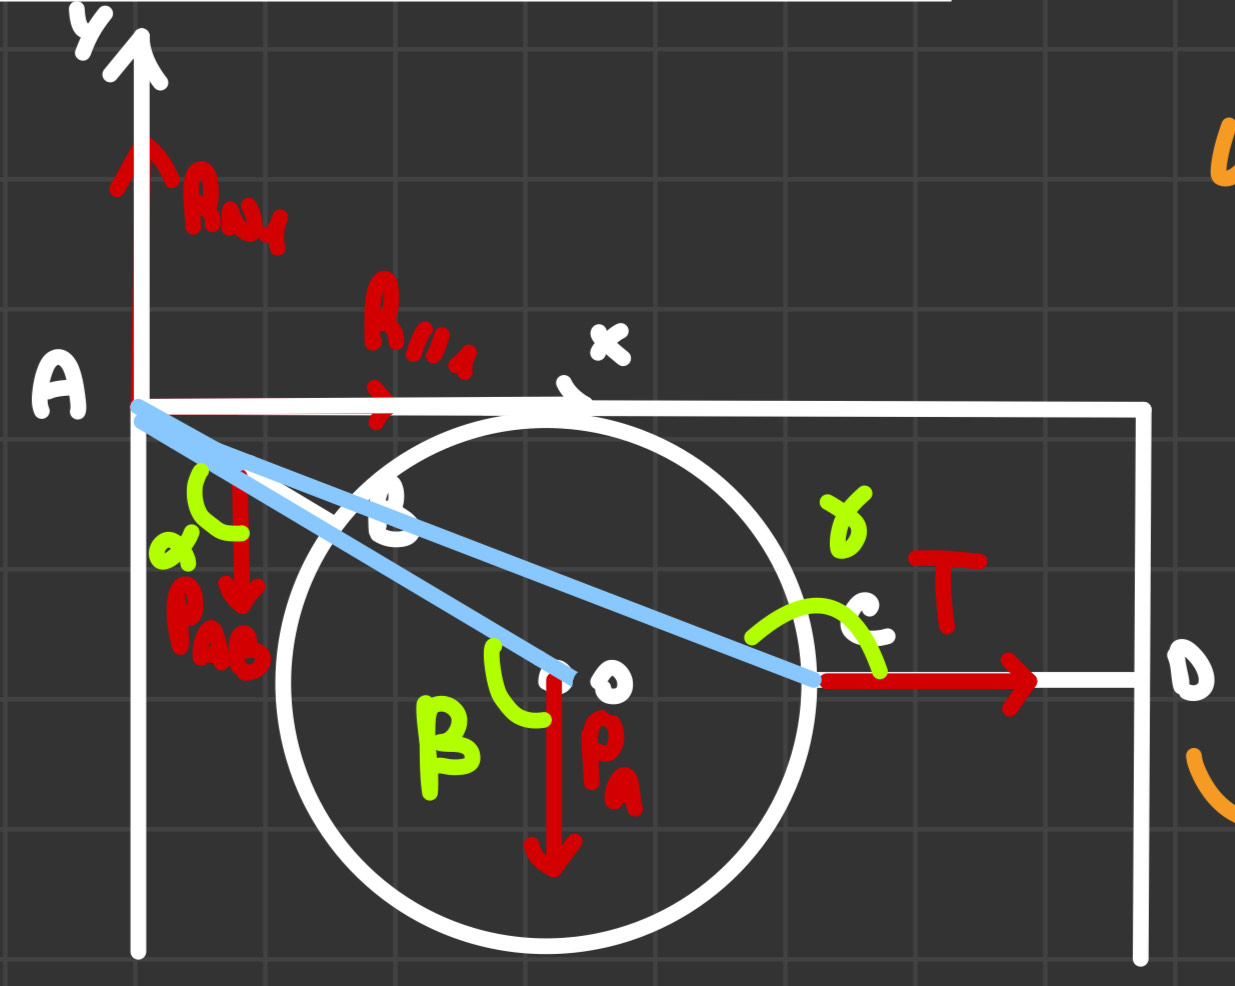
\includegraphics[width=0.4\linewidth]{PrimaFaseAstaEAnello.jpeg}
    \label{fig:placeholder}
\end{figure}
\noindent
Rispetto a questo disegno vi è da fare una precisazione, l'anello è appoggiata in alto al supporto, generalmente quando vi è un appoggio c'è sempre una reazione vincolare, in questo caso la parete dovrebbe essere spinta per reagire, se avessi avuto una forza che spingeva l'anello verso l'alto allora ci sarebbe stata una reazione vincolare verso il basso.
\subsubsection{Ricerca dei bracci}
Il primo braccio è abbastanza banale e corrisponde a metà dell'asta, il secondo braccio corrisponde all'asta più il raggio, ci resta da trovare il terzo. Analizziamo i due triangoli rettangoli evidenziati.
\begin{figure}[H]
    \centering
    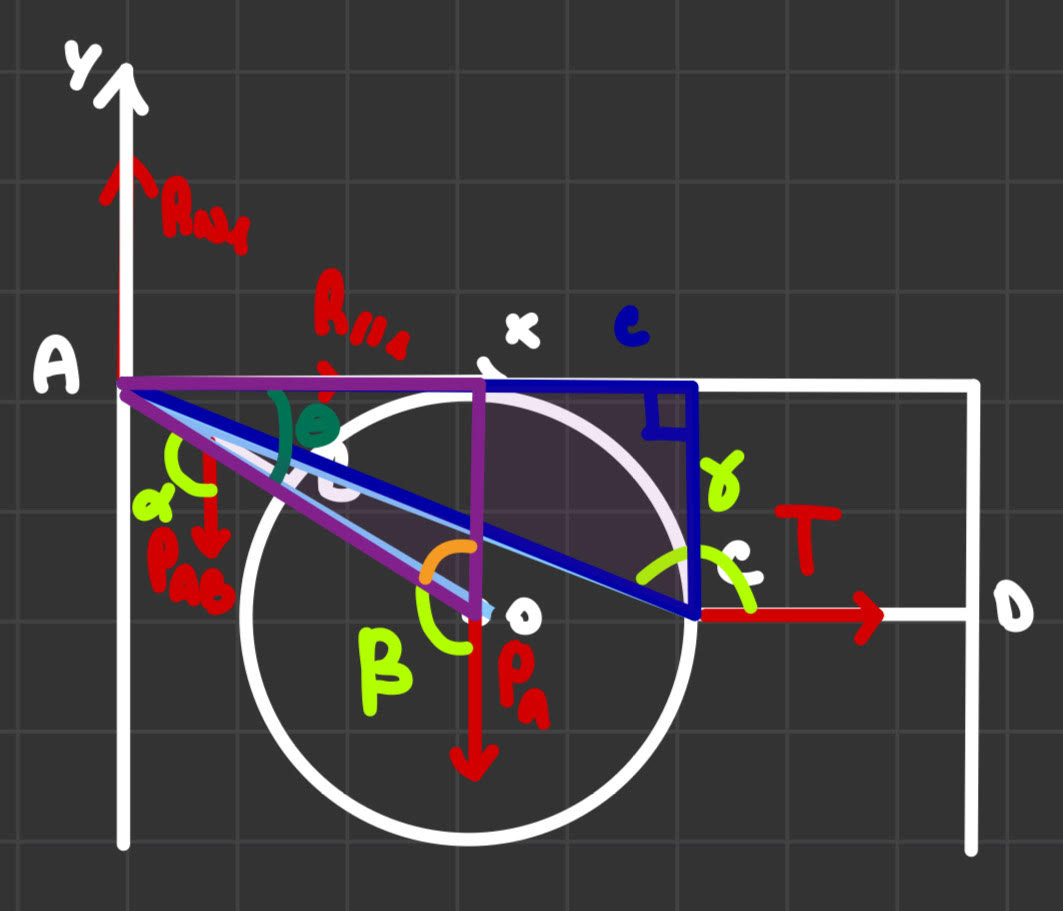
\includegraphics[width=0.4\linewidth]{SecondaFaseAstaAnello.jpg}
    \label{fig:placeholder}
\end{figure}
\noindent
Del triangolo rettangolo in blu, conosciamo l'altezza, ciò significa che se riuscissimo a determinare l'altro cateto riusciremmo a trovare il braccio mancante. Tracciando il triangolo in viola ci accorgiamo di qualcos'altro, il cateto c equivale a $c=r+b_2cos(\theta)$ dove il secondo termine rappresenta la proiezione di $b_2$ sull'orizzontale. Trovando $\theta$ con la trigonometria, riusciamo facilmente a trovare il cateto mancante e infine a trovare il braccio.
\subsubsection{Ricerca degli angoli}
Adesso dobbiamo fare delle osservazioni, nel disegno abbiamo disegnato solamente angoli ottusi, questo però ci risulta problematico, dato che vogliamo lavorare con \textbf{angoli acuti} per usare la trigonometria dei triangoli rettangoli. Tornando a quell'angolo sappiamo che si viene a creare tra il braccio e la direzione della forza, ciò significa che possiamo prendere anche il suo complementare, nel disegno di prima in \textbf{arancione}. $\beta$ lo troviamo facilmente con il triangolo in viola. $\alpha$ ha la direzione della forza uguale a $\beta$ e braccio che ha la stessa direzione di $\beta$, essendo gli angoli a due a due uguali vuol dire che $\alpha=\beta$ (in ogni caso potevamo trovarlo con lo stesso calcolo fatto per $\beta$ considerando il complementare di $\alpha$ nel disegno e chiudendo il triangolo rettangolo). Infine passiamo a $\gamma$ che conviene lasciare ottuso il quale è formato da 90 gradi + un certo $\gamma'$. $\gamma'$ lo possiamo trovare considerando il triangolo in blu, sappiamo infatti che se otteniamo l'angolo a sinistra possiamo ottenere anche $\gamma'$, quell'angolo lo otteniamo facilmente con la trigonometria. Altra soluzione consideriamo semplicemente $c=b_3sin(\gamma')$. Risolvo facilmente il sistema appena impostato.
\subsubsection{Ricerca della velocità angolare}
Qui andiamo a risolvere come detto prima con il \textbf{metodo energetico}. L'energia meccanica iniziale è puramente potenziale gravitazionale. In blu le altezze dei due corpi, i potenziali gravitazionali li otteniamo singolarmente e li andiamo semplicemente a sommare.
\begin{figure}[H]
    \centering
    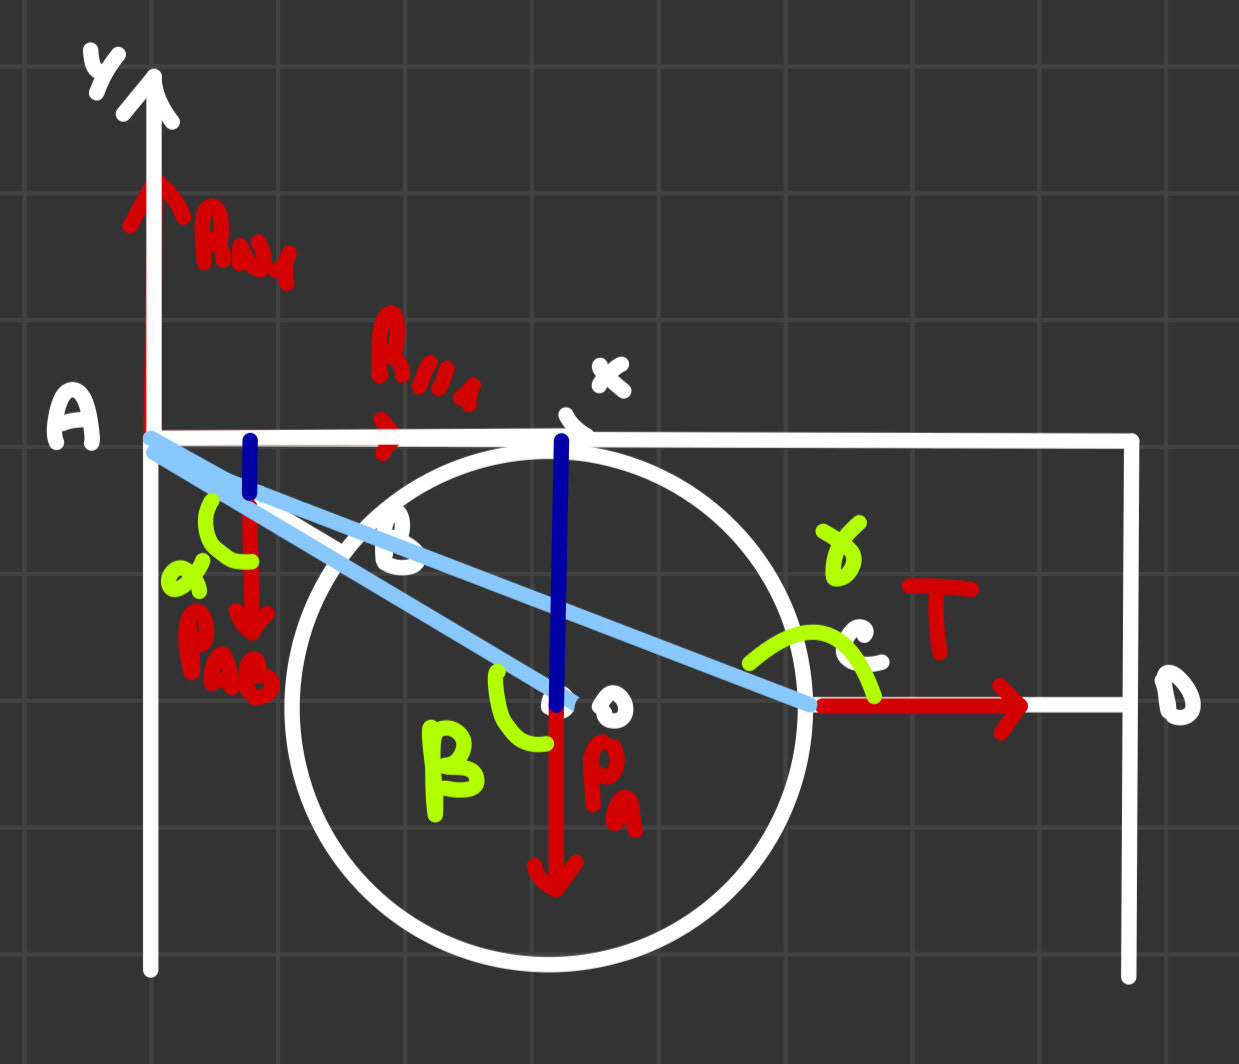
\includegraphics[width=0.5\linewidth]{TerzaParteAstaEAnello.jpg}
    \label{fig:placeholder}
\end{figure}
\noindent
L'altezza più grande la abbiamo, ci serve la più piccola che andiamo a calcolare semplicemente con il triangolo rettangolo più piccolo che viene a formarsi. Per l'istante finale la cosa da fare sempre è \textbf{avere il disegno della situazione finale}. Infatti disegnando mi accorgo che oltre ad avere una certa \textbf{energia cinetica rotazionale}, avrò anche una certa \textbf{energia potenziale gravitazionale}. Nota importante quello che succede è che \textbf{i triangoli sono sempre gli stessi solo che ruotano}. Le altezze infatti diventano quelle che prima erano le proiezioni dei bracci sull'orizzontale. Le calcolo, calcolo i momenti d'inerzia (faccio semplicemente la somma dei momenti) e trovo $\omega$.
\subsection{Problema dell'asta sui due piani inclinati}
\begin{figure}[H]
    \centering
    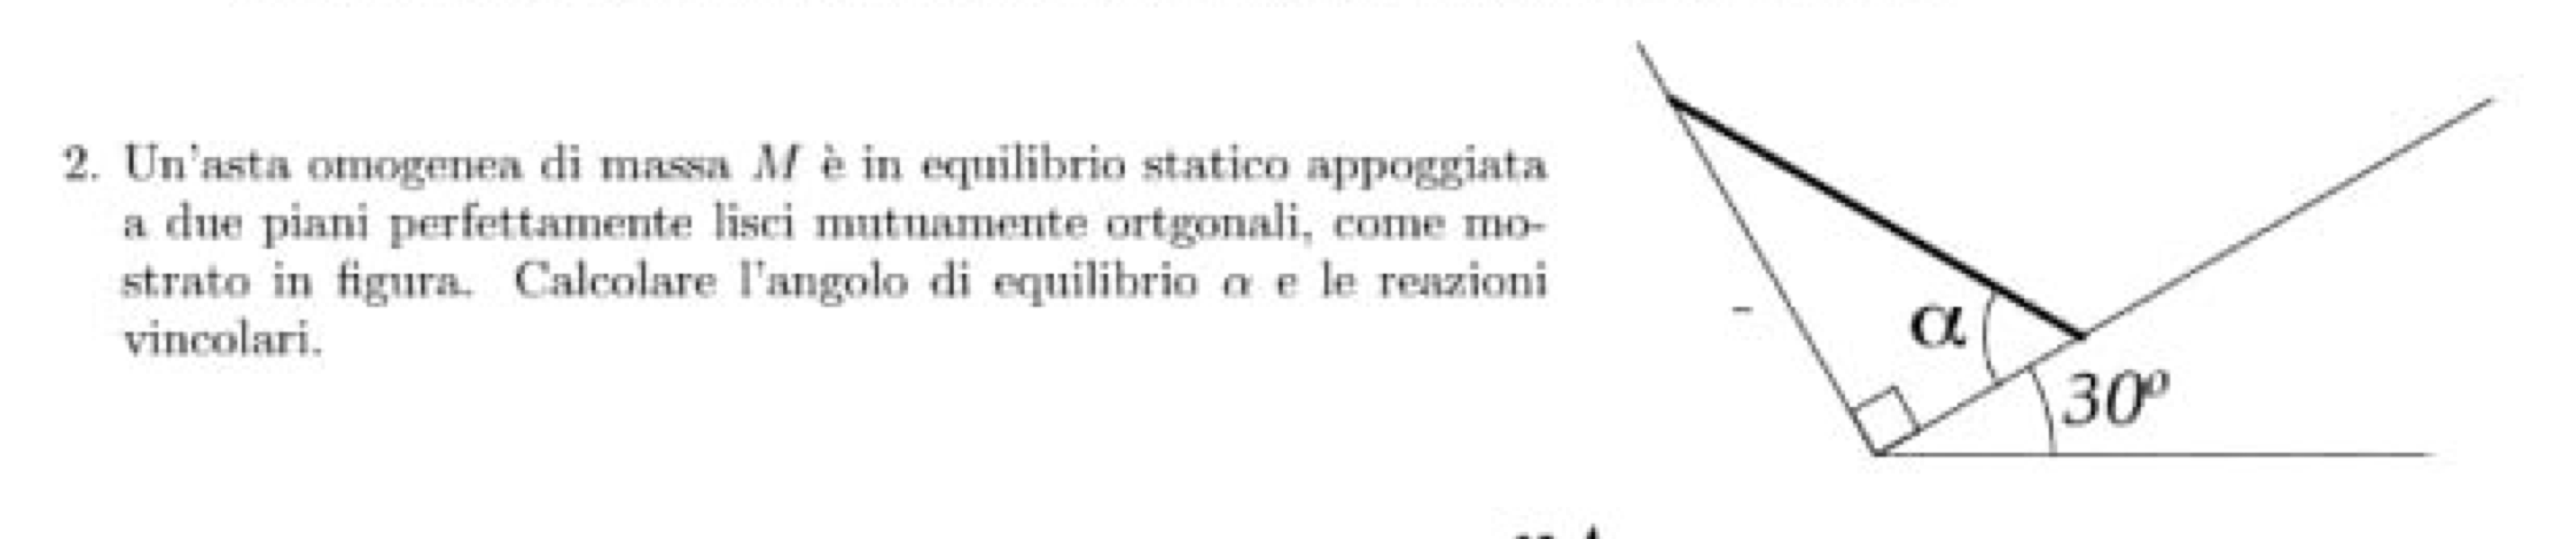
\includegraphics[width=0.7\linewidth]{AstaSuiPianiInclinati.png}
    \label{fig:placeholder}
\end{figure}
\noindent
Questo lo abbiamo solamente iniziato, nonostante ciò qui è da fare attenzione a mettere le reazioni vincolari \textbf{perpendicolari al piano}. Inoltre è un testo in cui non abbiamo molti dati ma abbiamo solamente informazioni sugli angoli, questo significa che dobbiamo lavorare su di essi. Imposto il sistema di equazioni con bracci e angoli.
\begin{figure}[H]
    \centering
    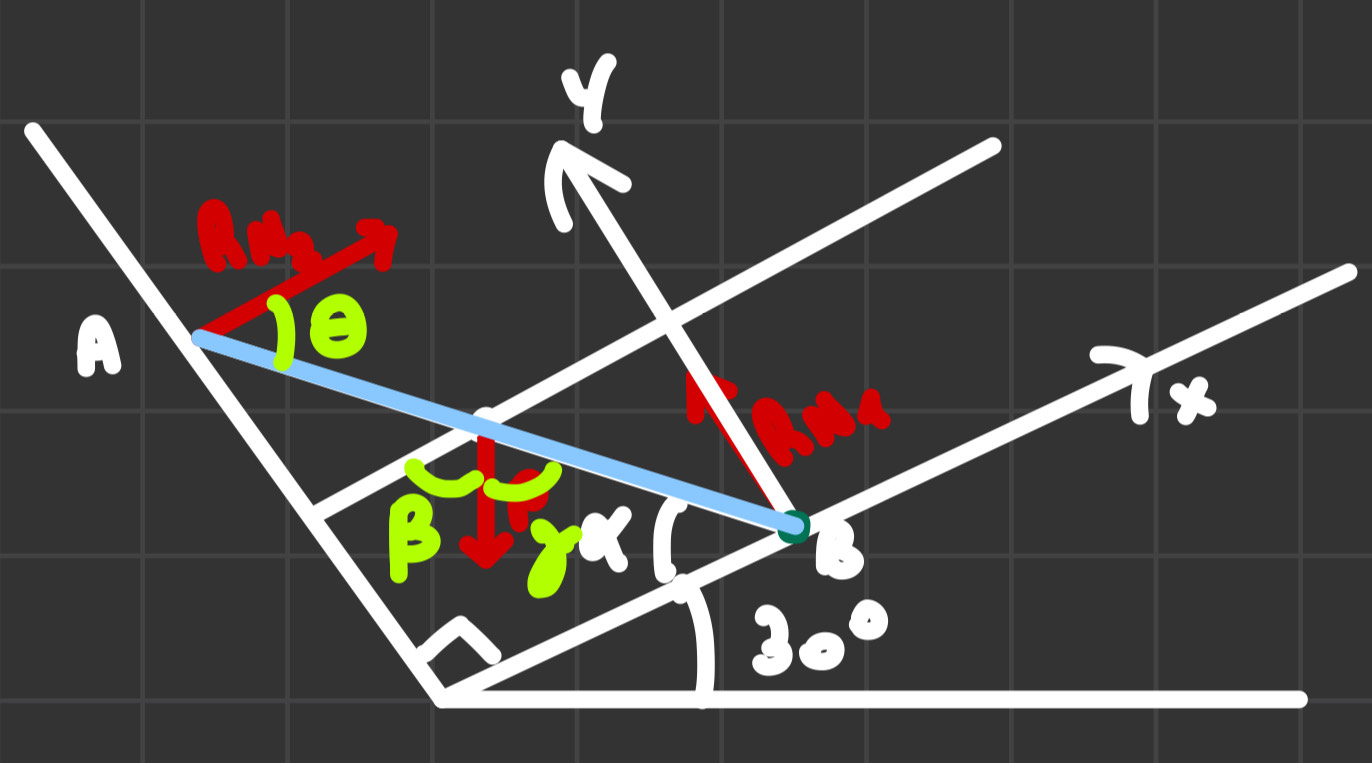
\includegraphics[width=0.5\linewidth]{PrimaFaseAstaSuiPiani.jpeg}
    \label{fig:placeholder}
\end{figure}
\noindent
\subsection{Ricerca degli angoli}
In questo caso i bracci "sono noti" infatti corrispondono a metà dell'asta e tutta la lunghezza dell'asta, quindi le incognite effettive sono le reazioni vincolari e gli angoli. $\beta$ si trova abbastanza facilmente con le \textbf{parallele tagliate dalla trasversale}, che in questo caso non sono altro che le \textbf{direzioni che formano $\beta$}.
\begin{figure}[H]
    \centering
    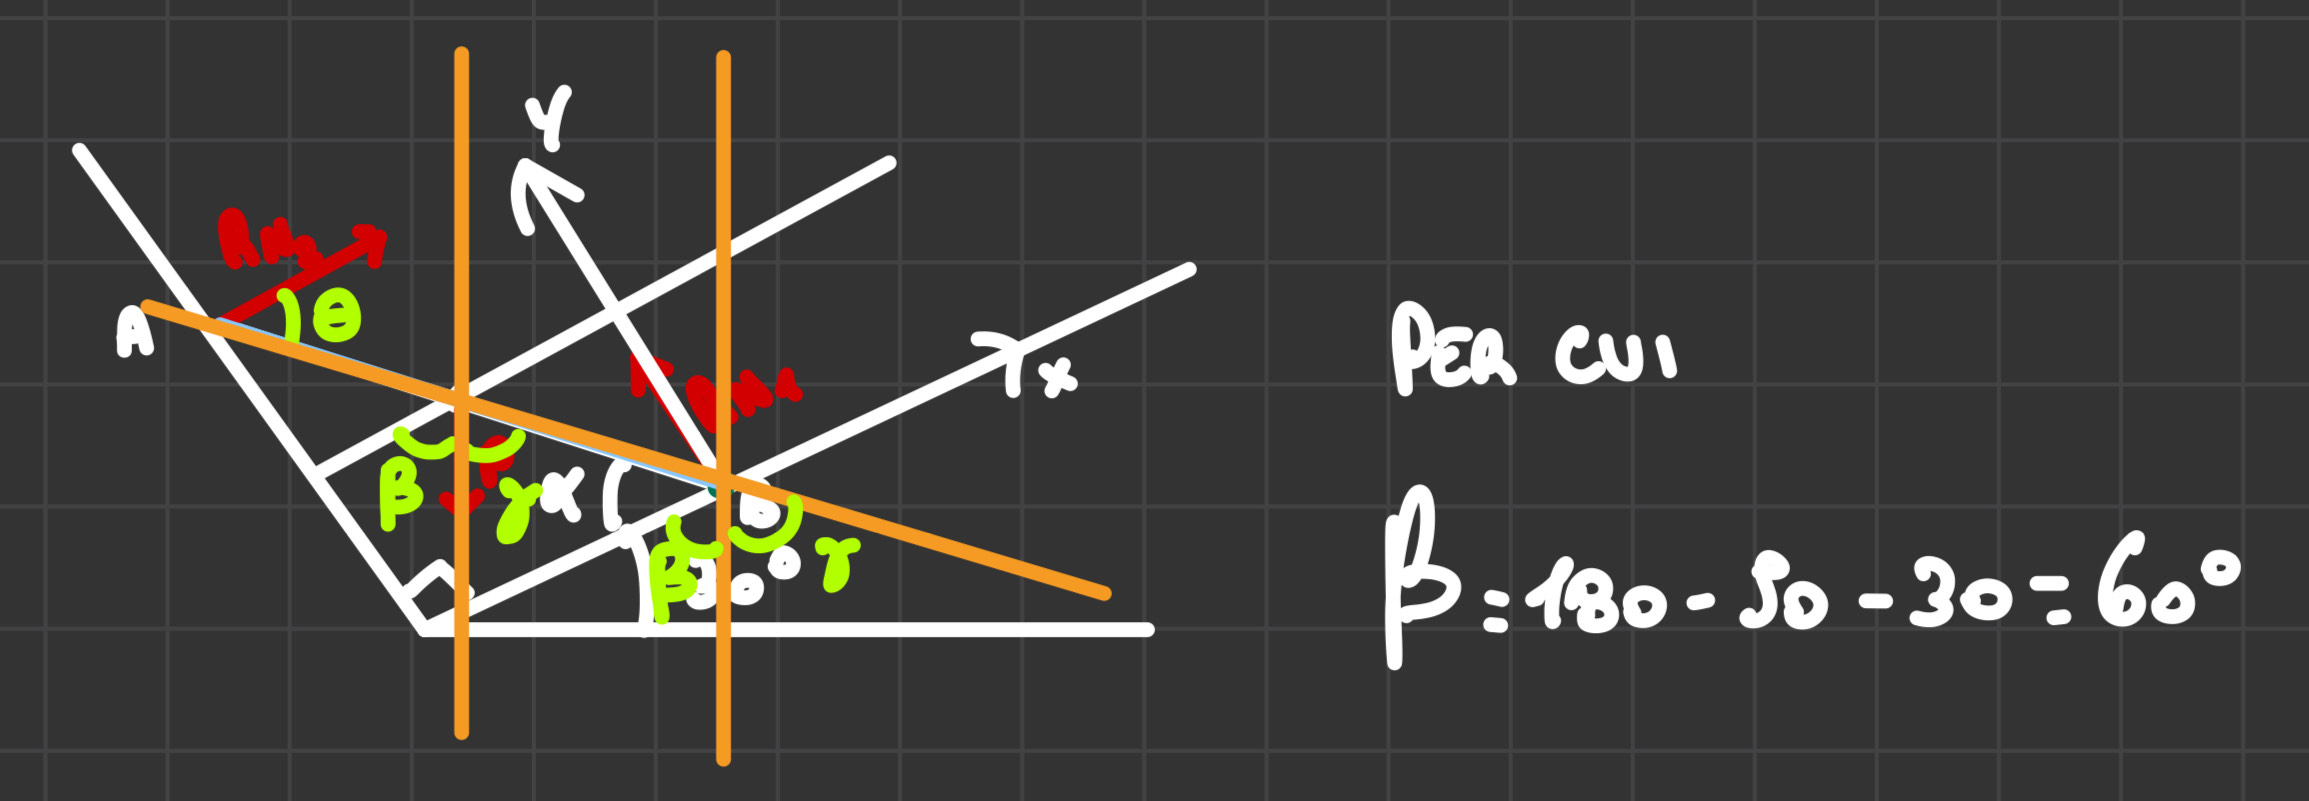
\includegraphics[width=0.5\linewidth]{SecondaFaseAstaSuiPiani.jpeg}
    \label{fig:placeholder}
\end{figure}
\noindent
Con le direzioni che formano $\alpha$ riesco a trovare un legame con $\beta \ \ e \ \ \gamma$.
\begin{figure}[H]
    \centering
    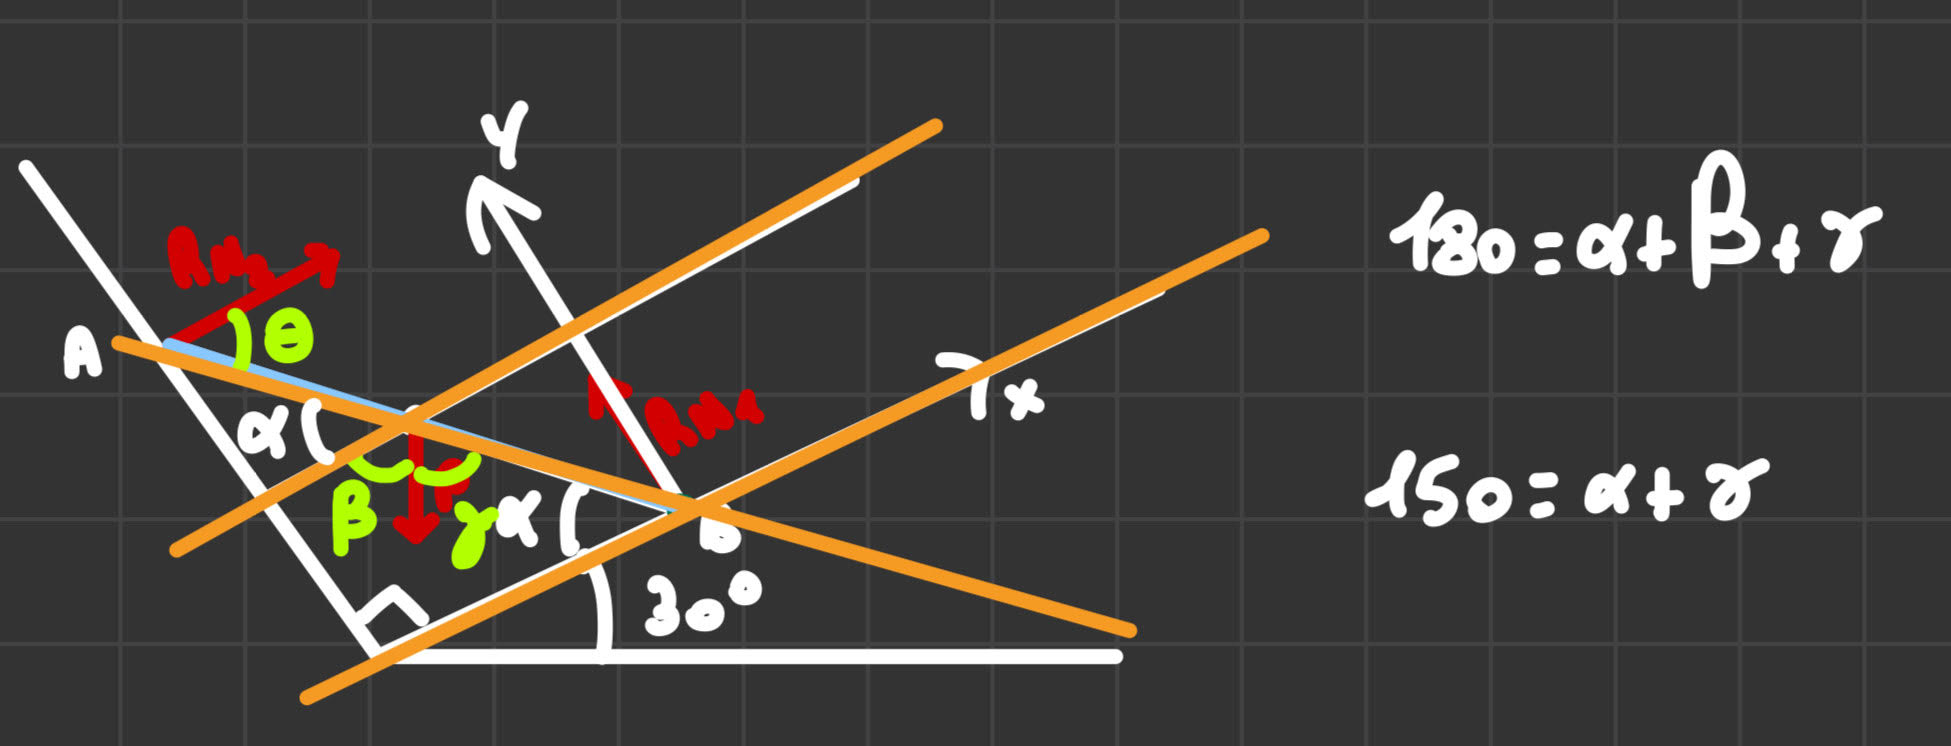
\includegraphics[width=0.5\linewidth]{TerzaFaseAstaSuiPiani.jpg}
    \label{fig:placeholder}
\end{figure}
\noindent
Con le direzioni di $\theta$ capisco che:
\begin{figure}[H]
    \centering
    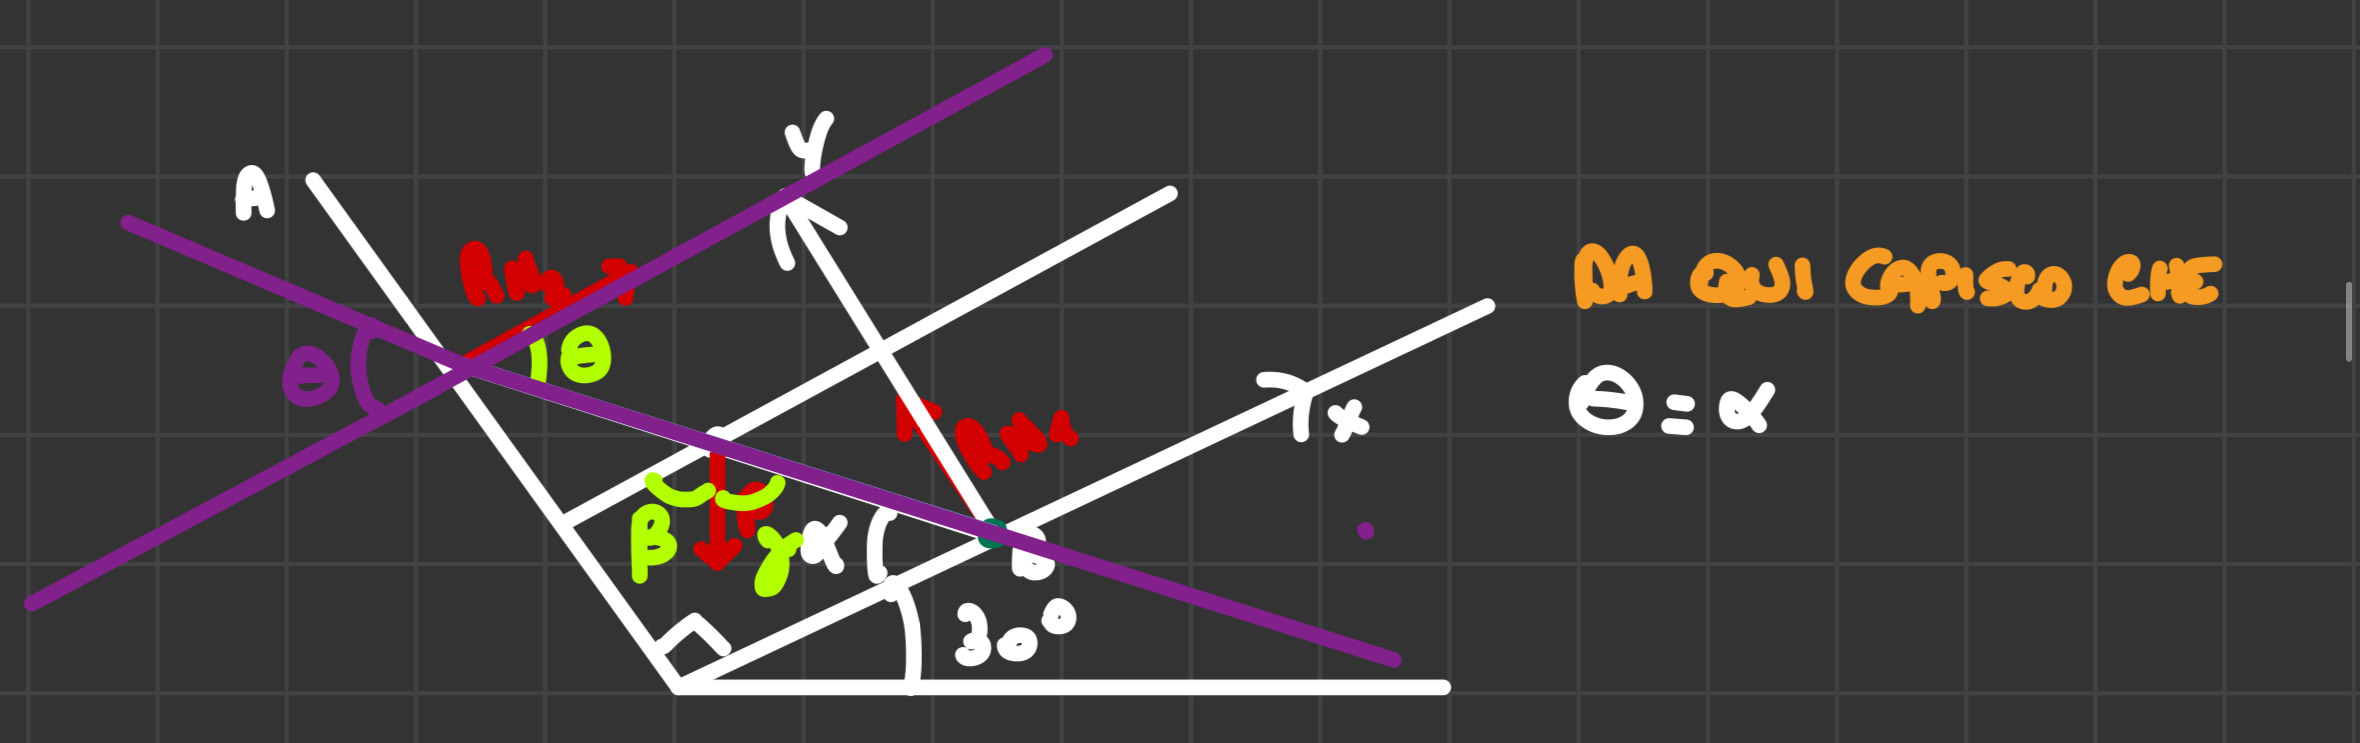
\includegraphics[width=0.5\linewidth]{QuartaFaseAstaSuiPiani.jpeg}
    \label{fig:placeholder}
\end{figure}
\noindent
Oltre al metodo delle direzioni e quello delle parallele tagliate dalla trasversale, abbiamo quello che \textbf{se le due direzioni sono a due a due perpendicolari gli angoli sono uguali}. Infatti per trovare $\gamma$, lo divido a metà notando che il pezzo sono ha le direzioni a due a due perpendicolari con l'angolo di 30 quindi sarà anche $\gamma''=30$. $\gamma'$ invece lo trovo facilmente dal triangolo rettangolo che si viene a formare. Risolvo il sistema e trovo le incognite.
\begin{figure}[H]
    \centering
    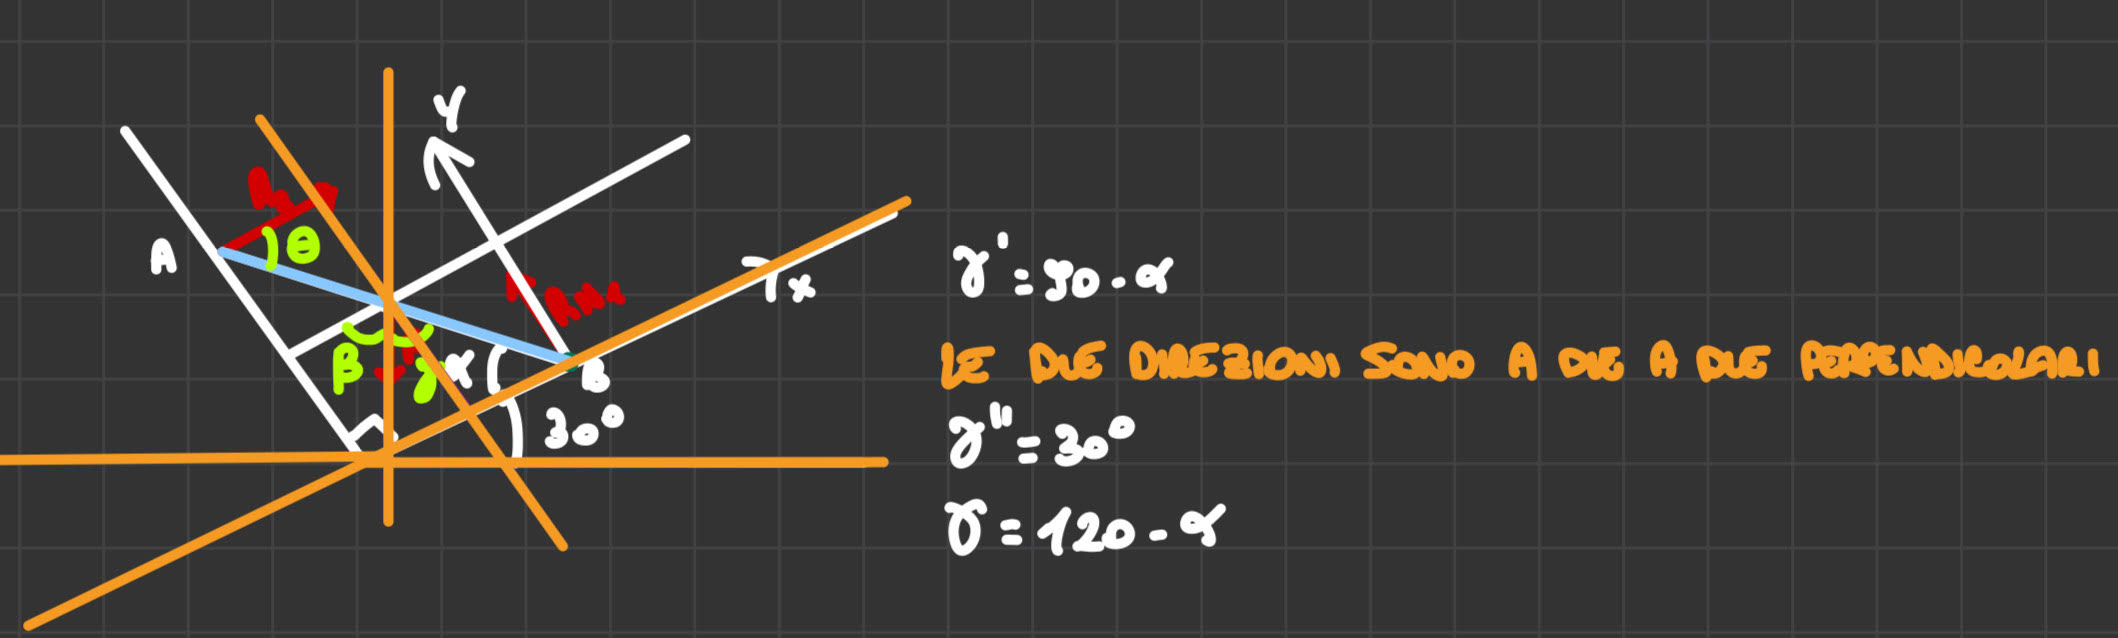
\includegraphics[width=0.5\linewidth]{QuintaFaseAstaSuiPiani.jpg}
    \label{fig:placeholder}
\end{figure}
\newpage
\section{Lezione 10}
In questa lezione andiamo a parlare dell'attrito e del suo ruolo con i corpi rigidi e degli esercizi sul moto parabolico, decidiamo di saltare le piccole oscillazioni dato che capitano meno frequentemente, torneremo sull'argomento.
\subsection{Problema delle aste con forza d'attrito}
\begin{figure}[H]
    \centering
    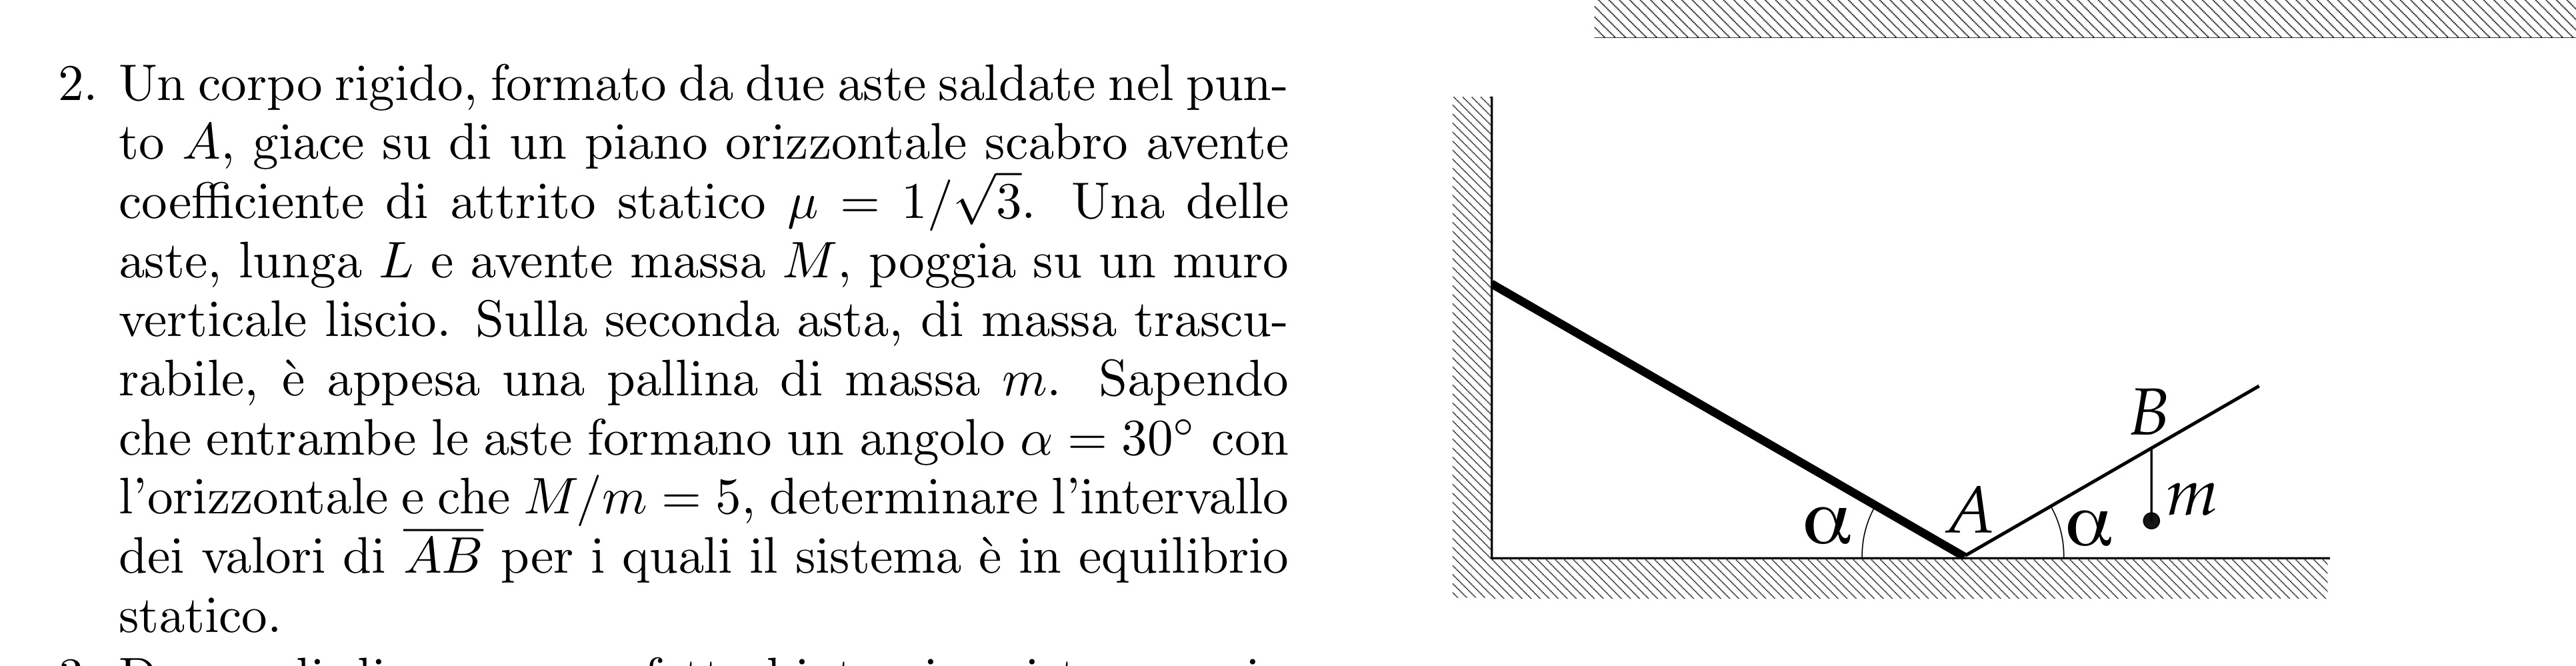
\includegraphics[width=0.7\linewidth]{ProblemaConAttrito.png}
    \label{fig:placeholder}
\end{figure}
\noindent
Capiamo un pochino come lavorare con la forza d'attrito, inizio come al solito a riportare tutte le forze in gioco, orientare gli assi dove conviene riportare bracci e angoli. Prima di fare un discorso sulla forza d'attrito vi è da notare come la seconda asta, risulta essere di massa trascurabile, per cui non vi sarebbe forza peso, nonostante ciò vi è una massa attaccata e quindi vi è forza peso, l'errore potrebbe essere quello di posizionare la forza peso a partire dalla massa, in realtà noi analizziamo tutto il sistema e il punto di applicazione dal punto di vista del sistema si trova sopra.
\begin{figure}[H]
    \centering
    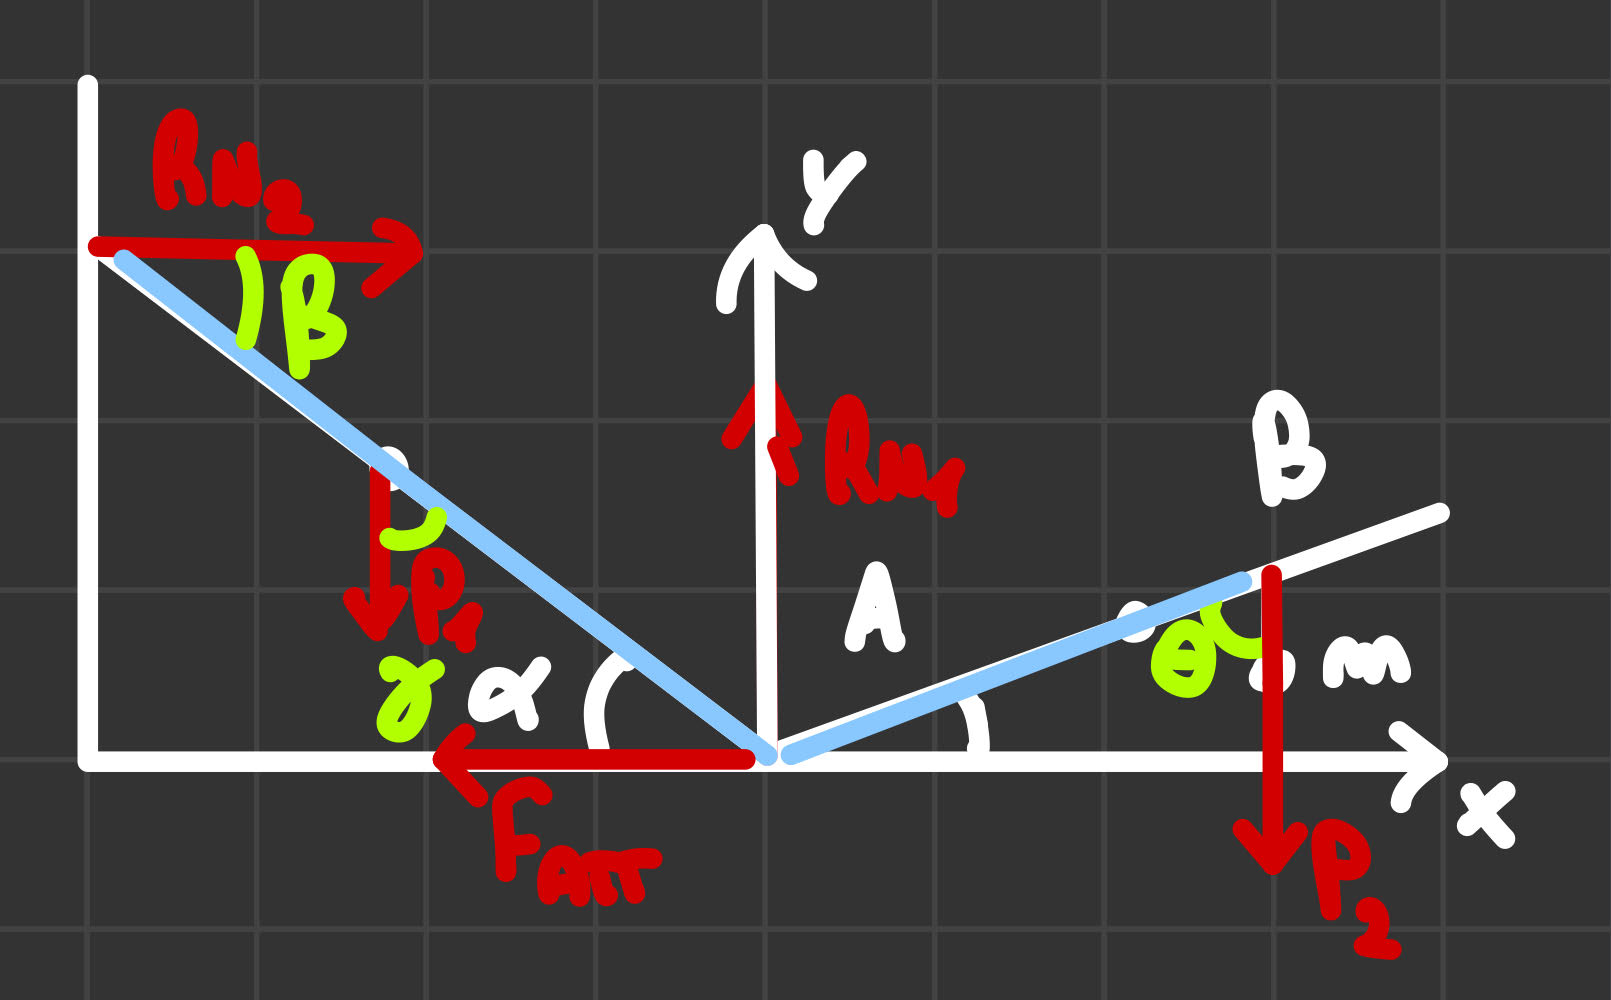
\includegraphics[width=0.5\linewidth]{PrimaFaseForzaD'Atrrito.jpg}
    \label{fig:placeholder}
\end{figure}
\noindent
\subsubsection{Lavorare con la forza d'attrito}
Bisogna considerare due cose quando andiamo a disegnarla, la forza d'attrito ha \textbf{direzione sempre parallela al piano}, il verso invece può esser scelto arbitrariamente, infatti in realtà anche quello delle reazioni vincolari viene scelto arbitrariamente. Iniziamo con la prima osservazione, quando un corpo è fermo, ricordiamo, l'attrito è incognito, infatti ha un valore che varia tra 0 e la forza d'attrito massima.
\subsubsection{Ricerca di bracci e angoli}
Questo non è un grande problema geometrico e bene o male si può trovare tutto abbastanza facilmente. Braccio 3 è la lunghezza dell'asta, braccio 2 è metà dell'asta, mentre braccio 1 è proprio l'incognita del problema. Per quanto riguarda gli angoli, $\gamma$ si trova facilmente con il triangolo formato dall'allungamento della forza peso, $\beta=\alpha$ dato che hanno le stesse direzioni e $\theta$ si trova facilmente come $\gamma$.
\subsubsection{Risoluzione del problema e riflessione sulla forza d'attrito}
Leggendo il problema si nota come esso chieda "determinare l'intervallo dei valori di AB per i quali il sistema è in equilibrio statico". Essendo un intervallo, sono presenti infiniti valori vogliamo quindi trovare i suoi estremi, per avere gli estremi però avremmo bisogno di due sistemi di equazioni. Da questa situazione si può uscire in due modi, o scrivo un'equazione che lega un'altra incognita, oppure \textbf{gioco con la forza d'attrito}. Infatti avrò un sistema al minimo e un sistema al massimo. Ovviamente al minimo la forza d'attrito vale 0. Al massimo bisogna fare attenzione, $F_{attr}=\mu N$, N non è detto che sia la forza peso, infatti N è la reazione vincolare  e per questo motivo \textbf{mettiamo come N la reazione vincolare nel punto di contatto}. In questo modo abbiamo legato la forza d'attrito a $R_{N1}$. Ovviamente capisco che c'è qualcosa che non va se mi vengono risultati assurdi come l'equazione impossibile o il braccio <0 in quel caso il risultato non è ammissibile. Risolvo il problema al minimo e al massimo.
\subsubsection{Richiesta tipo: è possibile l'equilibrio con l'attrito (incognita)?}
In questo caso si lavora in questo modo, trovo prima la reazione vincolare e poi l'attrito. Per leggere il risultato abbiamo che la $F_{attr, \ risultante}$ potrebbe essere $>F_{attr, \ max}$ infatti alla fine bisogna controllare se $F_{attr, \ risultante}<F_{attr,\ max}$. La forza d'attrito massima la calcolo come $F_{attr, \ max}=\mu N=\mu R_N$, dove la reazione vincolare è sempre quella nel punto di contatto.
\subsection{Esercizi sul moto parabolico}
\begin{figure}[H]
    \centering
    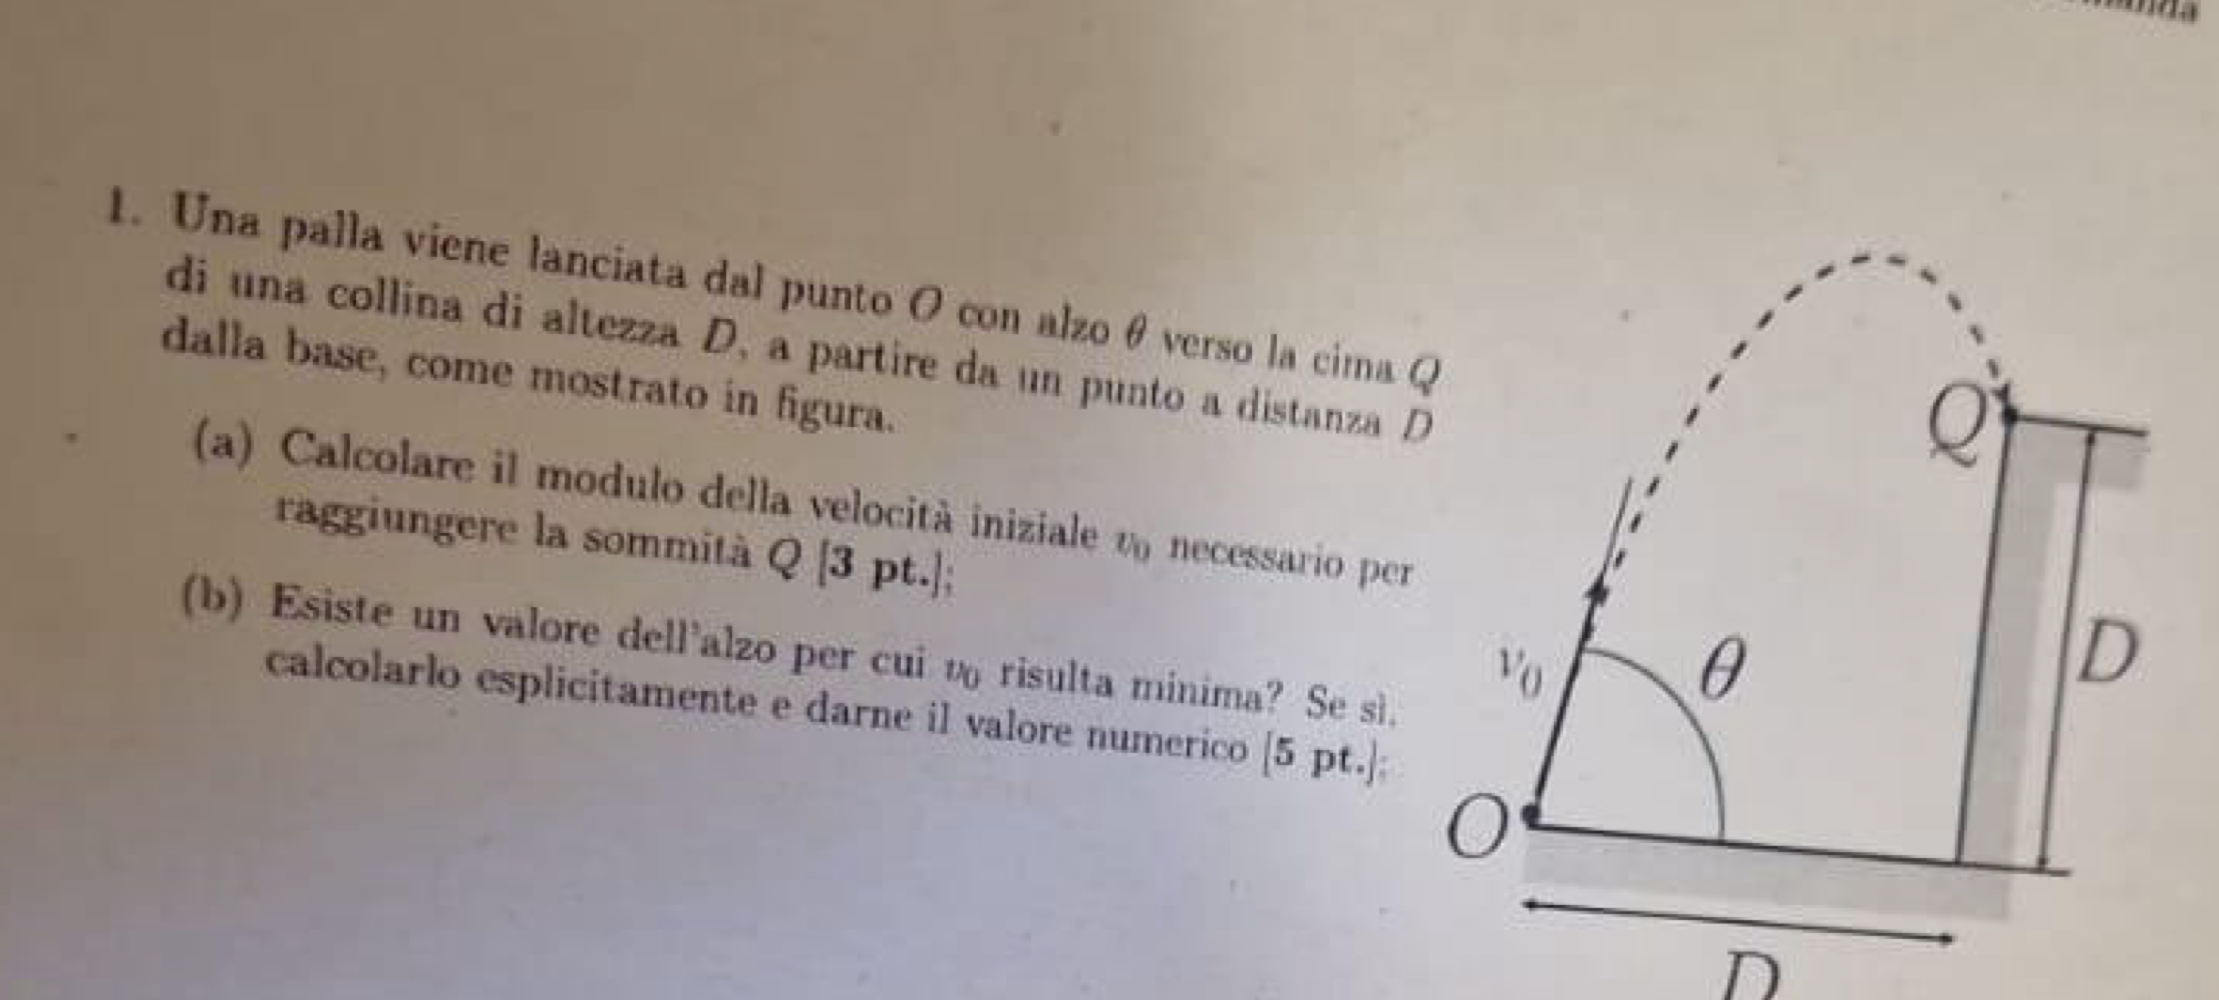
\includegraphics[width=0.6\linewidth]{PrimoEsercizioMotoParabolico.png}
    \label{fig:placeholder}
\end{figure}
\noindent
Fondamentale quando si lavora con il moto parabolico è \textbf{orientare gli assi da dove parte il punto}. Infatti oriento gli assi nel modo tradizionale e li piazzo nell'origine, lavoro con le leggi orarie sostituendo D a x e y, trovando t e $v_0$ in funzione dell'alzo (angolo).
\subsubsection{Minimizzare e massimizzare}
Come si osserva dalla seconda richiesta, viene richiesto un valore dell'alzo per cui la velocità risulta minima. Essendo $v_0$ in funzione di theta, questa diventa una funzione che va minimizzata. Nota: il discorso è analogo per quando la funzione va massimizzata. Come procedo, per prima cosa \textbf{semplifico la funzione al massimo}. In questo caso ho:
\begin{equation}
    v_0=\frac{D}{cos(\theta)\sqrt{\frac{D(tan(\theta)-1)}{4,9}}}
\end{equation}
Faccio entrare il coseno nella radice, poi dato che il numeratore non dipende da $\theta$ lo escludo e considero il denominatore, essendo la radice monotona posso minimizzare semplicemente il radicando, per quanto riguarda il denominatore della radice lo escludo non essendo in funzione di $\theta$ a questo punto \textbf{faccio la derivata, la pongo uguale a 0 e trovo l'angolo $\theta$}.
\begin{figure}[H]
    \centering
    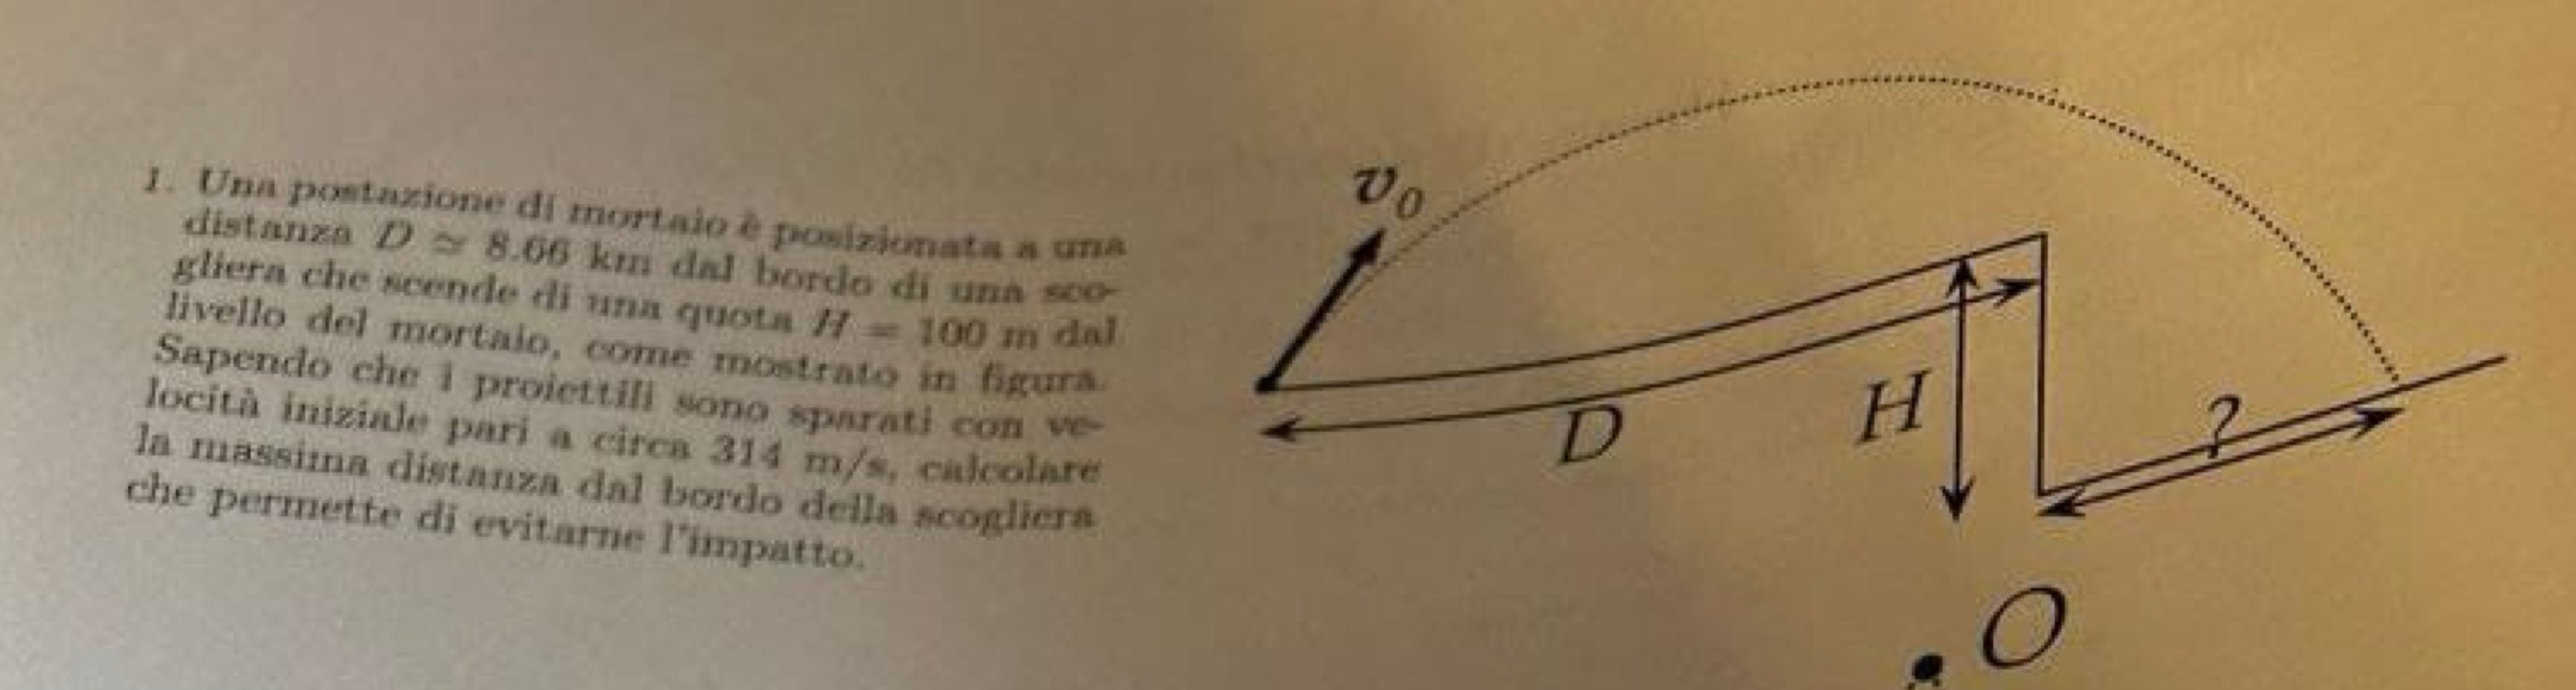
\includegraphics[width=0.5\linewidth]{ProblemaEvitareDiToccare.png}
    \label{fig:placeholder}
\end{figure}
\noindent
Anche qui, metto gli assi dove parte il punto facendo quindi attenzione a come imposto le leggi orarie. Osserviamo meglio la richiesta, "calcolare la massima distanza dal bordo della scogliera che permette di evitarne l'impatto", in realtà questo equivale a dire che il proiettile deve superare dunque è un \textbf{problema al limite} un pò come quando nel giro della morte imponevamo una \textbf{condizione al limite} e quindi al limite il \textbf{vertice della parabola deve passare per quel punto}. Imponiamo quindi le leggi orarie in quel punto (8660,0) e troviamo l'alzo. Una volta aver trovato l'alzo, possiamo continuare a lavorare sulle due equazioni senza sostituire la x e quindi trovare il tempo in funzione di x sostituirlo a la legge oraria di y e trovare x (massima distanza). Ci sarebbe da fare anche il problema del piano inclinato e dell'altezza ma lo avevo già risolto in autonomia, bisogna sempre fare attenzione a \textbf{posizionare gli assi dove parte il moto.}
\section{Lezione 11}
\subsection{Introduzione}
Iniziamo la parte di \textbf{termodinamica} che è quella scienza che \textbf{studia i movimenti del calore}.
\subsection{Principio 0 della termodinamica}
Il principio 0 della termodinamica ci dice che: due corpi che hanno diversa temperatura, si passano calore (energia in transito), il corpo più caldo passa calore al corpo più freddo fino a che i corpi non si posizionano in una \textbf{temperatura di equilibrio}. Raggiunto l'equilibrio non c'è più passaggio di calore e quindi anche corpi che hanno la stessa temperatura non si passano calore. Generalmente il passaggio di calore che consideriamo in fisica I è di tipo \textbf{conduttorio}: i due corpi sono in contatto.
\subsubsection{Corpi solidi, liquidi e gassosi}
Nei passaggi di calore vi è una differenza di temperatura in particolare:
\begin{itemize}
    \item 
\end{itemize}
\clearpage
\end{document}
